Определенное количество "--- {\em ближайшим образом} количество с некоторой
определенностью или границей вообще "--- есть в своей совершенной
определенности {\em число}. Определенное количество делится,

{\em во-вторых}, прежде всего {\em на экстенсивное} определенное количество,
в котором граница дана (ist) как ограничение налично сущего {\em множества},
а затем, когда это наличное бытие переходит в для-себя-бытие, на
{\em интенсивное} определенное количество, {\em градус}\footnote{Grad
по-немецки степень интенсивности, градус. В~большинстве случаев мы предпочли
передавать <<Grad>> не через <<степень>>, а через <<градус>>, чтобы избежать
смешения с <<Potenz>> (математическая степень), хотя <<градус>>, может быть,
несколько затушевывает качественный характер интенсивной величины. "---
{\em Перев}.}, которое, как <<для себя>> и в последнем как {\em безразличная
граница}, столь же непосредственно оказывается {\em вне себя}, имеет свою
определенность в некотором другом. Как это положенное противоречие, состоящее
в том, что оно, таким образом, просто определено внутри себя и вместе с тем
имеет свою определенность вне себя и отсылает за ней вне себя, определенное
количество,

{\em в-третьих}, как в самом себе внешне положенное, переходит
в~{\em количественную бесконечность}.

\section[А. Число]{А. Число}

Количество есть определенное количество или, иначе говоря, обладает границей
и как непрерывная и как дискретная величина. Различие этих видов пока что
не имеет здесь никакого значения.

Количество как снятое для-себя-бытие уже само по себе безразлично к своей
границе. Но тем самым ему также и не безразлично то обстоятельство, что оно
имеет границу или, другими словами, что оно есть некоторое определенное
количество; ибо оно содержит внутри себя одно, абсолютную определенность,
как свой собственный момент, который, следовательно, как положенный в его
(количества) непрерывности или единице, есть его граница, остающаяся,
однако, одним, которым она теперь вообще стала.

Это одно есть, стало быть, принцип определенного количества, но одно
{\em как количественное одно}. Благодаря этому оно, во-первых, непрерывно,
оно есть {\em единица; во-вторых}, оно дискретно, представляет собою
в-себе-сущее (как в непрерывной величине) или положенное (как в дискретной
величине) множество одних, которые одинаковы друг с другом, обладают
вышеуказанной непрерывностью, имеют одну и ту же единицу. {\em В-третьих},
это одно есть также и отрицание многих одних как простая граница, есть некое
исключение из себя своего инобытия, определение себя по отношению
к~{\em другим} определенным количествам. Постольку одно есть ($\alpha $)
{\em соотносящаяся с~собою} ($\beta $), {\em объемлющая и} ($\gamma $)
{\em исключающая другое} граница.

Определенное количество, полностью положенное в этих определениях, есть
{\em число}. Полная положенность заключается в наличном бытии границы как
{\em множества} и, стало быть, в ее отличности от единицы. Число представляется
поэтому дискретной величиной, но оно обладает также и непрерывностью в виде
единицы. Оно поэтому и есть определенное количество в совершенной
{\em определенности}, так как в числе граница выступает в виде определенного
{\em множества}, имеющего своим принципом одно, т.~е. нечто безоговорочно
определенное. Непрерывность, в каковой одно есть лишь {\em в~себе}, как снятое
(положенное как единица), есть форма неопределенности.

Определенное количество, лишь как таковое, ограничено вообще; его граница есть
его абстрактная, простая определенность. Но поскольку оно есть число, эта
граница положена как {\em многообразная в себе самой}. Число содержит в~себе те
многие одни, которые составляют его наличное бытие, но содержит их не
неопределенным образом, а определенность границы имеет место именно в нем;
граница исключает другое наличное бытие, т.~е. другие многие, и объемлемые ею
одни суть некоторое определенное множество, {\em численность}\footnote{Anzahl;
перевод через <<численность>> дан Лениным, хотя и предположительно и как один
из возможных переводов (см. <<Ленинский сборник>>~IX, стр.~82). Дебольский
переводит "--- <<определенное число>>; в томе~I Собрания сочинений Гегеля "---
<<определенное множество>>. "--- {\em Перев}.}, в~отношении которой как
дискретности, как она есть в числе, другим служит {\em единица}, его
непрерывность. {\em Численность и единица} составляют {\em моменты} числа.

Что касается численности, то следует еще рассмотреть ближе, каким образом
многие одни, из которых она {\em состоит}, заключены в границе. Относительно
численности правильно выражаются, говоря, что она {\em состоит} из многих, ибо
одни находятся в ней не как снятые, а {\em суть} в ней, только как положенные
вместе с исключающей границей, к которой они относятся безразлично. Но граница
не относится безразлично к ним. При рассмотрении нами наличного бытия отношение
к нему границы оказалось ближайшим образом таким, что наличное бытие как
утвердительное оставалось по сю сторону своей границы, а последняя, отрицание,
находилась вне его, у его края; точно так же во многих одних прерыв их и
исключение других одних выступает как некоторое определение, которое имеет
место вне объемлемых одних. Но там получился вывод, что граница пронизывает
наличное бытие, простирается столь же далеко, как последнее, и что нечто
вследствие этого ограничено по своему определению, т.~е. конечно. "---
В~области числовой количественности мы представляем себе, например, сто так,
что только сотое одно ограничивает многие таким образом, что они составляют
сто. С~одной стороны, это правильно; но, с другой стороны, среди ста одних
никакое из них не обладает преимуществом, так как они только одинаковы; каждое
из них есть в такой же мере сотое, как и другие; все они, следовательно,
принадлежат к той границе, благодаря которой данное число есть сто; для
получения своей определенности последнее не может обойтись ни без одного из
них; прочие одни, следовательно, не составляют в сравнении с сотым одним такого
наличного бытия, которое находилось бы вне границы или лишь внутри ее, вообще
было бы отлично от нее. Численность не есть поэтому некоторое множество в {\em
противоположность} объемлющему, ограничивающему одному, а сама составляет это
ограничивание, которое есть некоторое определенное количество; многие образуют
одно число, {\em одну} двойку, {\em один} десяток, {\em одну} сотню и~т.~д.

Итак, ограничивающее одно есть определенность в отношении другого, отличение
данного числа от других. Но это отличение не становится качественной
определенностью, а остается количественным, имеет место лишь в сравнивающей
{\em внешней} рефлексии. Число как одно остается обращенным назад к себе и
безразличным к другим. Это {\em безразличие} числа к другим есть его
существенное определение; оно составляет его {\em определенность в себе}, но
вместе с тем и {\em его собственную внешность}. "--- Число есть, таким образом,
{\em нумерическое} одно как абсолютно определенное, которое вместе с тем
обладает формой простой непосредственности и для которого поэтому соотношение с
другим является совершенно внешним. Как такое одно, которое есть {\em число},
оно, далее, имеет {\em определенность} (поскольку она есть {\em соотношение с
другим}) как свои моменты внутри самого себя, в своем {\em различии единицы и
численности}, и численность сама есть множество {\em одних}, т.~е. в нем самом
имеется этот абсолютно внешний характер. "--- Это противоречие числа или
определенного количества вообще внутри себя есть то качество определенного
количества, в дальнейших определениях которого (качества) это противоречие
получает свое развитие.

\hegremark[Примечание 1]%
  {Арифметические действия. Кантовские априорные синтетические суждения созерцания}%
  {[Арифметические действия. Кантовские априорные синтетические суждения созерцания]}

Пространственная и числовая величина обыкновенно рассматриваются как два
различных вида величин, причем понимают это различие таким образом, что
пространственная величина, взятая сама по себе, есть столь же определенная
величина, как и числовая величина. Их различие состоит согласно этому способу
рассмотрения лишь в определениях непрерывности и дискретности, как определенное
же количество они стоят на одной ступени. Геометрия имеет, говоря вообще, своим
предметом в виде пространственных величин непрерывную величину, а арифметика в
виде числовых величин "--- дискретную. Но вместе с этой неодинаковостью
предмета они также не обладают одинаковым способом и совершенством ограничения
или определенности. Пространственная величина обладает лишь ограничением
вообще; поскольку она должна рассматриваться как безоговорочно определенное
количество, она нуждается в числе. Геометрия как таковая не {\em измеряет}
пространственных фигур, не есть искусство измерения, она лишь {\em сравнивает}
их. В даваемых ею дефинициях определения также отчасти заимствуются ею из
{\em равенства} сторон, углов, из {\em равного} расстояния. Так, например,
круг, основывающийся единственно только на {\em равенстве} расстояния всех
возможных в нем точек от одной центральной точки, не нуждается для своего
определения ни в каком числе. Эти определения, основывающиеся на равенстве или
неравенстве, суть подлинно геометрические. Но их недостаточно, и для
определения других фигур, например, треугольника, четырехугольника требуется
число, заключающее в своем принципе, в одном, самостоятельную определяемость,
а не определяемость с помощью чего-то другого, стало быть, не определяемость
через сравнение. Пространственная величина имеет, правда, в точке
определенность, соответствующую одному; однако точка, поскольку она выходит вне
себя, превращается в другое, становится линией; так как она есть по существу
лишь одно {\em пространства}, то она в {\em соотношении} становится некоторой
такой непрерывностью, в которой снята точечность, самостоятельная
определяемость, одно. Поскольку самостоятельная определяемость должна
сохраниться во вне-себя-бытии, приходится представлять себе линию как некоторое
множество одних, и она должна получить внутри себя {\em границу}, определение
{\em многих} одних, т.~е. мы должны брать величину линии "--- и точно так же и
других пространственных определений "--- как число.

{\em Арифметика} рассматривает число и его фигуры, или, вернее сказать, не
рассматривает их, а оперирует с ними. Ибо число есть безразличная, косная
определенность; оно должно быть приведено в действие и в соотношение
{\em извне}. Способы этого соотнесения суть виды {\em арифметических действий}.
Они излагаются в арифметике одно после другого, и ясно, что одно {\em действие}
зависит от другого. Однако в арифметике не выделяется руководящая нить их
последовательности. Но из самого определения понятия числа легко получается тот
систематический порядок, на который справедливо притязает изложение этих
элементов в учебниках. На эти руководящие определения мы должны здесь вкратце
обратить внимание читателя.

Число есть вообще вследствие своего принципа, одного, некое внешне сочетанное,
всецело аналитическая фигура, в которой нет никакой внутренней связи. Так как
оно, таким образом, есть лишь некое порожденное извне, то всякое исчисление
есть продуцирование чисел, {\em считание} или, говоря более определенно,
{\em сосчитывание}. Разница в этом внешнем продуцировании, совершающем
постоянно лишь одно и то же, может заключаться единственно только в различии по
отношению друг к другу тех чисел, которые должны быть сосчитываемы; такое
различие само должно быть заимствовано из чего-то иного и из внешнего
определения.

Качественным различием, составляющим определенность числа, является то,
с~которым мы познакомились, а~именно, различие {\em единицы} и {\em численности;}
к этому различию сводится поэтому всякая определенность понятия, могущая иметь
место в арифметических действиях. Различие же, присущее числам как определенным
количествам, есть внешнее тождество и внешнее различие, {\em равенство} и
{\em неравенство}, которые суть рефлективные моменты и должны быть
рассматриваемы среди определений сущности там, где трактуется о различии.

Далее, нужно предпослать еще то замечание, что числа могут в общем быть
произведены двояким образом, либо через присовокупление
(Zu\-sam\-men\-fas\-sen), либо через разъединение уже присовокупленных;
поскольку этот двоякий способ произведения чисел имеет место при одинаковым
образом определенном виде считания, то совокуплению чисел (это можно назвать
{\em положительным} видом исчисления) соответствует некоторое определенное
разъединение их (это можно назвать {\em отрицательным} видом исчисления),
причем само определение вида исчисления независимо от этой противоположности.

После этих замечаний переходим к указанию видов исчисления.

1. Первым порождением числа является совокупление многих как таковых, т.~е.
многих, каждое из которых положено лишь как {\em одно}, "--- {\em нумерация}.
Так как одни внешни друг другу, то они представляются под каким-нибудь
чувственным образом и операция, посредством которой порождается число, есть
сосчитывание по пальцам, по точкам и~т.~п. Что такое четыре, пять и~т.~д., это
может быть лишь {\em показано}. Остановка в счете, будет ли совокуплено
столько-то одних или иное их количество, есть нечто случайное, произвольное,
так как граница внешня. "--- Различие численности и единицы, появляющееся в
дальнейшем развитии видов исчисления, служит основой {\em системы} чисел "---
двоичной, десятеричной и~т.~д.; такая система покоится в общем на произвольном
выборе той численности, которая постоянно должна снова и снова быть взята как
единица.

Возникшие посредством нумерации {\em числа} снова подвергаются нумерации; и
поскольку они положены так непосредственно, они еще определены без всякого
соотношения друг с другом, безразличны к равенству и неравенству, их величины
по отношению друг к другу случайны; они поэтому вообще {\em неравны;} это "---
{\em сложение}. "--- Что 7 и 5 составляют 12, это узнают таким образом, что к~7
принумеровывают на пальцах или как-нибудь иначе еще 5 одних, результат каковой
операции сохраняют затем в памяти, помнят {\em наизусть}, ибо здесь нет ничего
внутреннего. И~точно так же узнают посредством сосчитывания на пальцах и~т.~д.,
что $7\times 5=35$; знают это тем путем, что к одной семерке принумеровывается
еще одна семерка, повторяют это пять раз, и полученный результат также
запоминается наизусть. С~трудом этого нумерирования, нахождения сумм,
произведений навсегда покончено готовой таблицей сложения или умножения,
которую нужно лишь заучить наизусть.

Кант рассматривает (во Введении к <<Критике чистого разума>>, раздел~V)
предложение: $7+5=12$ как синтетическое предложение. <<Можно было бы, "---
говорит он, "--- сначала, правда, подумать (конечно!), что это чисто
аналитическое предложение, вытекающее, согласно закону противоречия, из
{\em понятия суммы} пяти и семи>>. Понятие суммы ничего более не означает,
кроме того абстрактного определения, что эти два числа {\em должны} быть
совокуплены и притом как числа внешним, т.~е. чуждым понятию образом, т.~е.
означает, что начиная с 7 следует продолжать нумерацию до тех пор, пока не
будут исчерпаны долженствующие быть прибавленными одни, численность которых
определена числом 5; полученный результат носит уже заранее известное название
двенадцати. <<Однако, "--- продолжает Кант, "--- при ближайшем рассмотрении мы
находим, что понятие суммы 7 и 5 ничего более не содержит в~себе, кроме
{\em соединения} этих двух чисел в одно единственное, чем вовсе еще
не~{\em мыслится, каково} это единственное число, соединяющее в себе те два
числа>>. <<Сколько бы я ни расчленял свое понятие о таковой возможной сумме, я
все-таки не встречу в нем двенадцати>>. С~{\em мышлением} суммы, с расчленением
понятия, переход от указанной задачи к получающемуся результату в самом деле не
имеет ничего общего. <<Нужно выйти за пределы этих {\em понятий}, прибегнуть к
помощи созерцания, пяти пальцев и~т.~д. и, таким образом, присоединить эти
единицы {\em данных в созерцании} пяти к {\em понятию} семи>>, "--- прибавляет
он. Пять в самом деле дано в созерцании, т.~е. есть совершенно {\em внешняя}
сочетанность произвольно повторявшейся мысли, одного; но 7 есть столь же мало
понятие; здесь нет понятий, за пределы которых нужно было бы выходить. Сумма 7
и 5 означает чуждое понятию соединение этих двух чисел; это столь чуждое
понятию нумерирование, продолжающееся от 7 до тех пор, пока не будут исчерпаны
пять единиц, можно назвать сочетанием, синтезированием ровно с таким же правом,
как и нумерацию, начинающую с одного, "--- синтезированием, которое, однако,
носит совершенно аналитический характер, так как связь здесь всецело
искусственная, в ней нет ничего такого и в нее не привходит ничего такого, что
не наличествовало бы перед нами совершенно внешним образом. Требование сложить
7 с 5 относится к требованию считать вообще как требование продолжить прямую
линию к требованию провести прямую линию.

Таким же бессодержательным, как выражение <<синтезирование>>, является
определение, что это синтезирование совершается a~priori. Правда, считание не
есть определение, принадлежащее области ощущений, которые согласно кантовскому
определению созерцания единственно только и остаются на долю a~posteriori, и
считание есть несомненно операция, совершающаяся на почве абстрактного
созерцания, т.~е. такого созерцания, которое определено категорией одного и при
котором абстрагируются как от всяких прочих определений, принадлежащих области
ощущения, так и от понятий. <<A~priori>> есть вообще нечто лишь смутное.
Определение, принадлежащее области эмоций "--- влечение, склонность и~т.~д.,
в такой же мере имеет в~себе момент априорности, а пространство и время как
существующие, т.~е. временное и пространственное, определены также и
à~posteriori.

В связи с этим мы можем прибавить, что в утверждении Канта о синтетическом
характере основоположений чистой геометрии также нет ничего основательного.
Признавая, что многие из них действительно аналитичны, он в доказательство
представления о синтетичности других приводит только ту аксиому, что прямая
линия есть кратчайшее расстояние между двумя точками. <<А~именно в~моем
{\em понятии} о прямой не содержится никакая величина, а содержится только
качество; {\em понятие} о кратчайшем расстоянии всецело, следовательно,
привходит извне, и никаким расчленением не может быть извлечено из
{\em понятия прямой линии;} здесь, следовательно, приходится брать себе в
помощь {\em созерцание} единственно лишь посредством которого возможен
синтез>>. "--- Но здесь дело вовсе и не идет о понятии прямого вообще, а о
прямой линии, последняя же есть уже нечто пространственное, созерцаемое.
Определение (или, если угодно, понятие) прямой линии ведь и состоит ни в чем
другом, как в том, что она есть {\em безоговорочно} простая линия, т.~е. в том,
что в своем выхождении вне себя (в так называемом движении точки) она
безоговорочно соотносится с собою, что в ее протяжении не положено никакой
разницы определения, никакого соотношения с некоторой другой точкой или линией
вне ее; она есть {\em безоговорочно простое внутри себя направление}. Эта
простота есть, разумеется, ее качество, и если кажется, что трудно дать
аналитическую дефиницию прямой линии, то это происходит лишь из-за определения
простоты или соотношения с самой собой и только потому, что при операции
определения рефлексия прежде всего имеет преимущественно в виду некую
множественность, операцию определения через другое. Но само по себе нисколько
не трудно понять это определение простоты протяжения внутри себя, отсутствие в
последнем определения через другое. Дефиниция Эвклида не содержит в себе ничего
другого, кроме этой простоты. "--- Но переход этого качества в количественное
определение (кратчайшего расстояния), который якобы составляет синтез,
исключительно и всецело аналитичен. Линия как пространственная есть количество
вообще; простейшим, что можно сказать об определенном количестве, является
<<{\em наименьшее}>>, а это последнее, высказанное о линии, есть
<<{\em кратчайшее}>>. Геометрия может брать эти определения как следствия из
дефиниции; но {\em Архимед} в своих книгах о шаре и цилиндре (см. перев.
{\em Гаубера}, стр.~4) поступил всего целесообразнее, выставив указанное
определение прямой линии как аксиому; он делает это в таком же правильном
смысле, в каком {\em Эвклид} поставил в числе аксиом определение, касающееся
параллельных линий, так как развитие этого определения для того, чтобы оно
стало дефиницией, также потребовало бы не непосредственно принадлежащих
пространственности, а более абстрактных качественных определений (подобно тому
как только что в применении к прямой линии потребовалось такое определение как
простота), "--- одинаковости направления и~т.~п. Эти древние сообщили также и
своей науке пластический характер, их изложение строго держалось своеобразия ее
материи и поэтому исключало из себя все, что было бы ему гетерогенно.

Понятие, которое Кант выставил в своем учении о синтетических суждениях
a~priori, "--- понятие о~{\em различном}, которое также и {\em неотделимо} друг
от друга, о~{\em тождественном}, которое в самом себе {\em нераздельно} есть
{\em различие}, принадлежит к тому, что есть великого и бессмертного в его
философии. В~созерцании это понятие, разумеется, также имеется, так как это
понятие есть само понятие, и всё есть в себе понятие; но те определения,
которые выделены в приведенных примерах, не выражают его; число и считание
есть, напротив, такое тождество и продуцирование такого тождества, которое
безоговорочно есть лишь внешнее тождество, лишь поверхностный синтез, единство
единиц, таких единиц, которые, напротив, положены как в самих себе не
тождественные друг с другом, а внешние, сами по себе раздельные. В~прямой линии
в основании определения, что она есть кратчайшее расстояние между двумя
точками, должен лечь скорее лишь момент абстрактного тождества, лишенного
различия в нем самом.

Я возвращаюсь от этого отступления к самому сложению. Соответствующий ему
отрицательный вид исчисления, {\em вычитание}, есть в~свою очередь совершенно
аналитическое отделение чисел, которые, как и в сложении, определены лишь как
вообще {\em неравные} в отношении друг друга.

2. Ближайшим определением является {\em равенство} тех чисел, над которыми
должно быть произведено действие нумерации. Благодаря этому равенству эти числа
суть {\em единицы}, и в числе появляется различие единицы и {\em численности}.
{\em Умножение} имеет задачей сосчитать воедино численность таких единиц,
которые сами суть тоже численности. При этом безразлично, какое из двух чисел
принимается за единицу и какое за численность, безразлично, говорим ли мы
четырежды три, где четыре есть численность, а три "--- единица, или, наоборот
трижды четыре. "--- Мы уже указали выше, что первоначальное нахождение
произведения совершается посредством простого процесса нумерации, т.~е.
сосчитывания на пальцах и~т.~д.; получающаяся позднее способность
{\em непосредственно} указать произведение покоится на собрании таких
произведений, на таблице умножения и знании ее наизусть.

{\em Деление} есть отрицательный вид исчисления согласно тому же определению
различия. Здесь также безразлично, какой из двух факторов, делитель ли или
частное, мы примем за единицу и какой за численность. Делитель принимается за
единицу, а частное "--- за численность, когда задачей деления объявляется
желание узнать, {\em сколько раз} (численность) некоторое {\em одно} число
(единица) содержится в данном числе; наоборот, делитель принимается за
численность, а частное за единицу в том случае, когда говорят, что требуется
разделить некоторое число на данную численность одинаковых частей и найти
величину такой части (единицы).

3. Те два числа, которые определены одно относительно другого как единица и
численность, еще непосредственны относительно друг друга и потому вообще {\em
неравны}. Дальнейшим равенством служит равенство самих единицы и численности;
таким образом, поступательное движение к равенству тех определений, которые
заключаются в определении числа, завершено. Считание согласно этому полному
равенству есть {\em возведение в степень} (отрицательным видом исчисления
служит здесь извлечение корня) и притом ближайшим образом возвышение
в~{\em квадрат;} это "--- полная определенность нумерирования внутри самого
себя, где (1) те многие числа, которые слагаются, суть одни и те же, и (2) само
их множество или численность тождественно тому числу, которое берется
многократно и служит единицей. Нет никаких иных определений в понятии числа,
которые могли бы представлять собою некоторое различие, и не может также иметь
место никакое дальнейшее выравнивание того различия, которое заключается
в~числе. Возведение в степени высшие, чем вторая, есть {\em формальное}
продолжение, которое отчасти "--- при четных показателях "--- есть лишь
{\em повторение} возведения в квадрат, и отчасти "--- при нечетных показателях
"--- есть появление снова прежнего неравенства; а именно, при формальном
равенстве (например, ближайшим образом в кубической степени) нового множителя
как с численностью, так и с единицей, он как единица представляет собою нечто
неравное по отношению к численности (по отношению к второй степени, 3 "--- по
отношению к $3/times 3$); еще большее неравенство имеется при кубической
степени четырех, где численность (3), показывающая, сколько раз число, служащее
единицей, должно быть помножено само на себя, отлична от последнего. "--- Эти
определения имеются сами по себе, как существенное различие понятия, "---
численность и единица, и для того, чтобы выход из себя вполне возвратился в
себя, они должны быть выравнены. В~только что изложенном заключается, далее,
основание, почему, с одной стороны, решение уравнений высших степеней должно
состоять в приведении их к квадратным уравнениям и, почему, с другой стороны,
уравнения нечетных степеней могут быть определены лишь формально, и как раз,
когда корни рациональны, они могут быть найдены не иначе, как при помощи мнимых
выражений, представляющих собою противоположность того, что суть и выражают
собою корни. "--- Согласно сказанному единственно только арифметический квадрат
содержит в себе всецелую определенность, вследствие чего уравнения дальнейших
формальных степеней должны быть приведены к нему; точно так же, как в геометрии
прямоугольный треугольник содержит в себе всецелую определенность внутри себя,
выраженную в пифагоровой теореме, и поэтому для полного определения всех прочих
геометрических фигур они должны быть приведены к нему.

В преподавании, подвигающемся вперед согласно логически построенному суждению,
изложение учения о степенях предшествует изложению учения о пропорциях;
последние, правда, примыкают к различию единицы и численности, составляющему
определение второго вида исчисления, однако они выходят за пределы того одного,
которое есть одно {\em непосредственного} определенного количества, в котором
единица и численность суть лишь моменты; дальнейшее определение по этим
моментам\pagenote{В немецком тексте вместо слов <<nach denselben>> (по ним,
т.~е. по этим моментам) стоят слова <<nach demselben>> (по нему). По-видимому,
это опечатка.} остается для него самого также еще внешним. Число в отношении не
есть уже {\em непосредственное} определенное количество; последнее имеет тогда
свою определенность как опосредствование; количественное\pagenote{В немецком
тексте вместо слова <<quantitative>> (количественное) стоит слово
<<qualitative>> (качественное). По-видимому, это опечатка.} отношение мы
рассмотрим далее.

О вышеуказанном все дальнейшем и дальнейшем определении арифметических действий
можно сказать, что оно не есть философствование о них, не есть, скажем,
изложение их внутреннего значения, потому что оно на самом деле не есть
имманентное развитие понятия. Но философия должна уметь различать то, что по
своей природе есть внешний самому себе материал, должна знать, что в таком
материале поступательное движение понятия может происходить лишь внешним
образом и что моменты этого движения могут иметь бытие лишь в своеобразной
форме их внешности, какова здесь форма равенства и неравенства. Различение
сфер, к которым принадлежит та или другая определенная форма понятия, т.~е.
сфер, в которых она имеется как существование, служит существенным условием
философствования о реальных предметах, необходимым для того, чтобы мы идеями не
нарушали своеобразия внешнего и случайного и чтобы мы вместе с том не искажали
этих идей и не делали их формальными вследствие несоответственности материала.
Но тот внешний характер, который носит выступление моментов понятия в
вышеуказанном внешнем материале, в числе, есть здесь соответственная форма; так
как они представляют нам предмет в присущем ему смысле, а также ввиду того, что
они не требуют никакого спекулятивного подхода и потому представляются легкими,
они заслуживают применения в элементарных учебниках.

\hegremark[Примечание 2]%
  {Употребление числовых определений для выражения философских понятий}%
  {[Употребление числовых определений для выражения философских~понятий]}

Как известно, {\em Пифагор} изображал в {\em числах разумные отношения} или
{\em философемы}, да и в новейшее время философия применяла числа и формы их
соотношений; как, например, степени и~т.~п., чтобы регулировать согласно им или
выражать в них мысли. "--- В педагогическом отношении число признавалось
наиболее подходящим предметом внутреннего созерцания, а занятие вычислением его
отношений "--- деятельностью духа, в которой он делает наглядными свои
наисобственнейшие отношения и вообще основные отношения сущности. "--- В~какой
мере числу на самом деле принадлежит эта высокая ценность, видно из его
понятия, каким оно получилось выше.

Число обнаружилось для нас как абсолютная определенность количества, а его
стихия "--- как ставшее безразличным различие; оно оказалось определенностью
в~себе, которая вместе с~тем положена лишь вполне внешне. Арифметика есть
аналитическая наука, так как все встречающиеся в ее предмете связи и различия
не зависят от него самого, а учинены ему совершенно извне. Она не имеет
конкретного предмета, который содержал бы в себе внутренние отношения,
первоначально скрытые для знания, не данные в непосредственном представлении
о~нем, а долженствующие быть выявлены усилиями познания. Она не только не
содержит в себе понятия и, следовательно, задачи для постигающего в понятиях
(für das begreifende) мышления, но есть его противоположность. Вследствие
безразличия приведенного в связь к связи, которой недостает необходимости,
мышление оказывается здесь занятым деятельностью, которая вместе с тем есть
самое крайнее отчуждение от самого себя, занятым насильственной деятельностью,
заключающейся в том, что оно {\em движется} в сфере {\em безмыслия} и приводит
в связь то, что не способно носить характер необходимости. Предметом здесь
служит абстрактная мысль о~{\em внешности} как таковой.

Будучи такой {\em мыслью} о внешности, число есть вместе с тем абстракция от
чувственного многообразия; от чувственного оно ничего другого не сохранило,
кроме абстрактного определения внешности; благодаря этому в числе чувственное
наивозможно ближе подведено к мысли. Число есть {\em чистая мысль} о
самоотчуждении мысли.

Поднимающийся над чувственным миром и познающий свою сущность дух, ища стихии
для своего чистого {\em представления}, для {\em выражения своей сущности},
может поэтому раньше, чем он постигнет, что сама мысль является этой стихией и
обретет для ее изображения чисто духовное выражение, вздумать избрать для этого
{\em число}, эту внутреннюю, абстрактную внешность. Поэтому мы находим в
истории науки, что уже рано применяли число для выражения философем. Оно
составляет последнюю ступень того несовершенства, которое состоит в том, что
всеобщее берется как обремененное чувственным. Древние определенно сознавали,
что число находится посередине между чувственным и мыслью. Согласно Аристотелю
(<<Метафизика>>, 1, 5) {\em Платон} говорил, что помимо чувственного и идей,
посередине между ними, находятся математические определения вещей; от
чувственного они отличаются тем, что они невидимы (вечны) и неподвижны, а от
идей "--- тем, что они суть некоторое множественное и сходное, между тем как
идея лишь безоговорочно тождественна с собою и едина внутри себя. "--- Более
подробное, основательно продуманное рассуждение об этом Модерата Кадиксского
приводится в <<Malchi vita Pythagorae ed. Ritterhus>>, стр.~30 и~сл.; то
обстоятельство, что пифагорейцам пришла в голову мысль остановиться на числах,
он приписывает тому, что они еще не были в состоянии {\em ясно} постигнуть в
{\em разуме} основные идеи и первые начала, потому что трудно продумать и
выразить эти начала; числа хорошо служат для обозначения при преподавании;
пифагорейцы, между прочим, подражали в этом геометрам, которые, не умея
выражать телесное в мысли, применяют фигуры и говорят, что {\em это} "---
треугольник, причем они требуют, чтобы не принимали за треугольник лежащий
перед глазами чертеж, а лишь представляли себе с помощью последнего мысль о
треугольнике. Так, например, пифагорейцы выразили как {\em одно} мысль о
единстве, тождественности и равенстве, а также и основание гармонии, связи и
сохранения всего, основание тождественного с самим собою и~т.~д. "--- Излишне
заметить, что пифагорейцы перешли от выражения в числах также и к выражению в
мыслях, к определенно названным категориям равного и неравного, границы и
бесконечности; уже касательно вышеуказанного выражения в числах сообщается (там
же, в примечаниях к стр.~31 цитированного издания, взятых из <<Жизни Пифагора>>
у Фотия, стр.~722), что пифагорейцы различали между монадой и единицей; монаду
они принимали за мысль, а единицу за число; и точно так же и число два они
принимали за арифметическое выражение, а диаду (ибо таково, видимо, то
название, которое оно у них носит) "--- за мысль о неопределенном. "--- Эти
древние, во-первых, очень ясно усматривали неудовлетворительность числовой
формы для выражения определений мысли, и столь же правильно они, далее,
требовали настоящего выражения мысли вместо того первого выражения, являвшегося
только крайним выходом; насколько опередили они в своих размышлениях тех,
которые в наше время снова считают чем-то похвальным и даже основательным и
глубоким замену определений мысли самими числами и такими числовыми
определениями, как, например, степенями, а затем "--- бесконечно большим,
бесконечно малым, единицей, деленной на бесконечность, и прочими подобного рода
определениями\pagenote{Имеются в виду Шеллинг и его последователи в
натурфилософии.}, которые даже и сами по себе часто представляют собою
превратный математический формализм, "--- считают основательным и глубоким
возвращение к вышеупомянутому беспомощному детству.

Что касается вышеприведенного выражения, что число занимает промежуточное
положение между {\em чувственным} и мыслью, имея вместе с~тем то общее с
первым, что оно есть по своей природе (an ihr) {\em многое}, внеположное, то
следует заметить, что само это многое, принятое в мысль чувственное, есть
принадлежащая ей (мысли) категория внешнего в самом себе. Дальнейшие,
конкретные, истинные {\em мысли}, представляющие собою наиболее живое, наиболее
подвижное, только {\em соотнесением и занимающееся}, превращаются в мертвенные,
неподвижные определения, когда их перемещают в эту стихию вне-себя-бытия. Чем
богаче становятся мысли определенностью и тем самым также и соотношением, тем
более запутанным, с одной стороны, а с другой стороны, тем более произвольным и
лишенным смысла становится их изложение в таких формах, как числа. Единица,
два, три, четыре, генада или монада, диада, триада, тетрактис, еще близки к
совершенно {\em простым}, {\em абстрактным} понятиям; но когда числа должны
переходить к изображению конкретных отношений, тогда оказывается тщетным
стремление сохранить связь между ними и понятием.

А когда для характеристики движения понятия, благодаря каковому движению оно
только и есть понятие, обозначают определения мысли через одно, два, три,
четыре, то этим предъявляется к мышлению самое жестокое требование. Мышление
движется тогда в стихии своей противоположности, отсутствия соотношений. Его
дело становится тогда работой безумия. Постигнуть, например, что одно есть три,
а три "--- одно, потому так трудно, что одно есть нечто лишенное соотношений и,
следовательно, не являет в самом себе того определения, посредством которого
оно переходило бы в свою противоположность, а, напротив, состоит именно в
полном исключении такого рода соотношения и отказе от него. Рассудок, наоборот,
пользуется этим против спекулятивной истины (например, против истины,
заключающейся в учении, называемом учением о триединстве) и {\em перечисляет}
те определения последней, которые составляют одно единство, чтобы выставить ее
как явную бессмыслицу, т.~е. он сам впадает в бессмыслицу, превращая в лишенное
соотношений то, что всецело есть соотношение. Слово <<триединство>>
употребляется, конечно, не в расчете на то, что рассудок будет рассматривать
{\em одно} и число как {\em существенную} определенность содержания. Это слово
выражает собою презрение к рассудку, который в своем тщеславии, однако, упорно
держится одного и числа как таковых и выставляет это тщеславие как оружие
против разума.

Принимать числа, геометрические фигуры просто за {\em символы}, как это часто
проделывали с кругом, треугольником и~т.~д. (круг, например, принимался за
символ вечности, треугольник "--- за символ триединства), есть, с одной
стороны, нечто совершенно невинное; но нелепо, с другой стороны, предполагать,
что этим выражают нечто большее, чем то, что {\em мысль} способна {\em
постигнуть и выразить}. Если в таких символах, как и в других, создаваемых {\em
фантазией} в народной мифологии и вообще в поэзии, в сравнении с которыми
чуждые фантазии геометрические фигуры сверх того скудны, "--- если в самом деле
и в первых и в последних заключается глубокая мудрость, глубокое {\em
значение}, но это как раз исключительно задача мышления сделать явной мудрость,
которая в них лишь {\em сокрыта} (darin liegt) и притом сокрыта не только
в~них, но и в природе и духе. В~символах истина в силу чувственного элемента
еще {\em помутнена} и {\em закутана;} она вполне открывается сознанию только
в~форме мысли; их {\em значением} служит лишь сама мысль.

Но заимствование математических категорий с целью что-нибудь определить
относительно метода или содержания философской науки уже потому оказывается по
существу чем-то превратным, что, поскольку математические формулы обозначают
мысли и различия понятия, это их значение, наоборот, должно быть сначала
указано, определено и оправдано в философии. В~своих конкретных науках
последняя должна почерпать логическое из логики, а не из математики. Обращение
для установления логического в философии к тем формам (Gestaltungen), которые
это логическое принимает в других науках и из которых многие суть только
предчувствия, а другие "--- даже искажения этого логического, может быть лишь
крайним средством, к которому прибегает философское бессилие. Голое применение
таких заимствованных формул есть сверх того внешний способ действия; самому
применению должно было бы предшествовать осознание как их ценности, так и их
значения; но такое осознание дается лишь мыслительным рассмотрением, а не
авторитетом, который эти формулы получили в математике. Таким их осознанием,
является сама логика, и это осознание совлекает их частную форму, делает ее
излишней и никчемной, исправляет ее, и исключительно лишь оно сообщает им
оправдание, смысл и ценность.

Какое значение имеет употребление числа и счета, поскольку оно должно
составлять главную {\em педагогическую} основу, это из предшествующего само
собою ясно. Число есть нечувственный предмет, и занятие им и его сочетаниями
"--- нечувственное занятие; дух, следовательно, этим приучается к рефлексии
в~себя и к внутренней абстрактной работе, что имеет большое, но одностороннее
значение. Ибо, с другой стороны, так как в основании числа лежит лишь внешнее,
чуждое мысли различие, то указанная работа становится безмысленной,
механической. Требуемое ею напряженное усилие состоит преимущественно в том,
чтобы удерживать чуждое понятию, и комбинировать его, не прибегая к понятию.
Содержанием здесь служит пустое одно; богатое содержание (der gediegene Inhalt)
нравственной и духовной жизни и индивидуальных ее образований, которое, как
благороднейшая пища, должно служить великим средствам воспитания юношеского
духа, вытесняется бессодержательной единицей. Результатом этих упражнений,
когда их делают главным делом и преимущественным занятием, может быть только
то, что дух по форме и содержанию опустошается и притупляется. Так как счет
есть столь внешнее и, стало быть, механическое занятие, то оказалось возможным
изобрести {\em машины}, совершеннейшим образом выполняющие арифметические
действия. Если бы о природе счета было известно хотя бы только одно это
обстоятельство, то одним этим был бы решен вопрос, какова ценность зряшной
мысли сделать счет главным средством воспитания духа и этим подвергать его
пытке, заставляя его усовершенствовать себя до того, чтобы стать машиной.

\section[B. Экстенсивное и интенсивное определенное количество]%
  {B. Экстенсивное и интенсивное определенное количество}

\subsection[a) Различие между ними]{a) Различие между ними}

1. Определенное количество, как оказалось в предшествующем, имеет свою
определенность как границу в численности. Оно есть некое в себе дискретное,
некое множественное, не имеющее такого бытия, которое было бы отлично от его
границы и имело бы ее вне себя. Определенное количество, взятое таким образом
со своей границей, которая есть некое многообразное в себе самой, есть
{\em экстенсивная величина}.

Следует отличать {\em экстенсивную} величину от {\em непрерывной}. Первой
непосредственно противоположна не {\em дискретная}, {\em а интенсивная}
величина. Экстенсивная и интенсивная величины суть определенности сам\'{о}й
количественной {\em границы}, определенное же количество тождественно со своей
границей. Непрерывная и дискретная величины суть, напротив, определения
{\em величины в себе}, т.~е. количества как такового, поскольку мы, имея дело
с определенным количеством, отвлекаемся от границы. "--- Экстенсивная величина
имеет момент непрерывности в самой себе и в своей границе, так как ее
множественное есть вообще непрерывное; постольку граница как отрицание
выступает {\em в этом равенстве} многих как ограничение единства. Непрерывная
величина есть продолжающее себя количество безотносительно к какой бы то ни
было границе, и, поскольку мы ее представляем себе с таковой границей,
последняя есть некое ограничение вообще, {\em без того чтобы в нем была
положена дискретность}. Определенное количество, взятое лишь как непрерывная
величина, еще не определено истинно для себя, так как в ней отсутствует одно,
от которого зависит то обстоятельство, что имеется определенность для себя,
а~также отсутствует и число. И~точно так же дискретная величина есть
непосредственно лишь различенное многое вообще, которое, поскольку оно как
таковое должно было бы иметь границу, было бы только некоторым множеством (eine
Men\-ge), т.~е. некоторым неопределенно ограниченным; чтобы оно получило
определенность определенного количества, для этого требуется совокупление
многих воедино, благодаря чему они полагаются тождественными с границей.
Каждая, и непрерывная и дискретная, величина, как {\em определенное количество}
вообще, положила в себе (an ihr) лишь одну из тех двух сторон, которыми оно
вполне определено и благодаря которым оно становится {\em числом}. Последнее
есть непосредственно {\em экстенсивное} определенное количество, {\em простая}
определенность, которая есть по существу численность, однако численность одной
и той же {\em единицы;} оно отлично от числа только тем, что определенность
в~последнем явно положена как множественность.

2. Однако определение величины посредством числа не нуждается в отличии от
какой-либо другой величины, так что выходило бы, что для определенности этой
величины требуются она сама и некоторая другая величина; она в этом не
нуждается потому, что определенность величины есть вообще
для-себя-определенная, безразличная, просто с собою соотнесенная граница, а
в числе она положена, как заключенная в для-себя-сущее одно, и имеет внешность,
соотношение с другим, {\em внутри самой себя}. Далее, само это присущее границе
многое, как и многое вообще, есть не неравное внутри себя, а непрерывное.
Каждое из многих есть то же самое, что другое; поэтому оно, как многое, сущее
друг вне друга или дискретное, не образует определенности как таковой. Это
многое, стало быть, сливается само по себе в свою непрерывность и становится
простым единством. "--- Численность есть лишь момент числа, но {\em не как
множество нумерических одних} оно {\em составляет} определенность числа, а эти
одни как безразличные, внешние себе, сняты в возвращенности числа в себя.
Внешность, составлявшая характер одних во множестве, исчезает в одном как
соотношении числа с самим собою.

Граница определенного количества, которое как экстенсивное имело свою налично
сущую определенность в виде внешней самой себе численности, переходит,
следовательно, в {\em простую определенность}. В~этом простом определении
границы оно есть {\em интенсивная величина;} и граница или определенность,
которая тождественна с определенным количеством, теперь так и положена как
простое; это "--- {\em градус}.

Градус есть, следовательно, определенная величина, определенное количество, но
не вместе с тем множество (Menge) или много [одних] {\em внутри самого себя;}
он есть только некая {\em многость} (Mehrheit), причем {\em многость} есть
многое, сжатое (zusammengenommen) в~{\em простое} определение, наличное бытие,
перешедшее обратно в для-себя-бытие. Его определенность должна быть, правда,
выражена некоторым {\em числом} как полной определенностью определенного
количества, но она дана не как {\em численность}, а просто есть лишь один
градус. Когда говорят о десяти, двадцати градусах, определенное количество,
имеющее столько градусов, есть десятый, двадцатый градус, а не численность и
сумма этих градусов, "--- в таком случае оно было бы экстенсивным количеством,
"--- а оно есть лишь один градус, десятый, двадцатый градус. Он содержит в себе
определенность, заключающуюся в численности <<десять>>, <<двадцать>>, но
содержит их не как многие, а есть число как {\em снятая} численность, как
простая {\em определенность}.

3. В~числе определенное количество положено в своей полной определенности; а
как интенсивное определенное количество (которое представляет собою
для-себя-бытие числа) определенное количество положено таким, каково оно
согласно своему понятию или в себе. А~именно, та форма соотношения с собою,
которую оно имеет в градусе, есть вместе с тем его
{\em внебытие относительно себя}. Число как
экстенсивное определенное количество есть нумерическая множественность и
имеет таким образом внешность внутри себя; эта последняя, как многое
вообще, сжимается в неразличимость и снимает себя в том обстоятельстве, что
число есть одно (in dem Eins der Zahl), в соотношении числа с самим собою.
Но определенное количество имеет свою определенность в виде численности;
оно, как было указано выше, содержит ее в себе, хотя она уже больше не
положена в нем. Таким образом, {\em градус}, который,
как простой внутри самого себя, уже больше {\em не
имеет} этого {\em внешнего инобытия внутри себя}, имеет
его {\em вне себя} и соотносится с ним как со своей
определенностью. Внешняя ему множественность составляет определенность той
простой границы, которой он сам по себе является. Что численность, которая
в экстенсивном определенном количестве должна была находиться внутри числа,
сняла себя в градусе, это определяется, следовательно, далее, так, что она
положена вне его. Поскольку число положено как одно, как рефлектированное в
себя соотношение с собою самим, оно исключает из себя безразличие и внешний
характер численности и есть {\em соотношение с собою
как соотношение посредством самого себя с чем-то внешним}.

В этом определенное количество получает соответственную своему понятию
реальность. {\em Безразличие} определенности составляет
его качество, т.~е. определенность, которая в самой себе дана как внешняя
себе определенность. "--- Согласно этому градус есть простая определенность
величины {\em среди} некоторого
{\em множества} таких интенсивностей, которые суть
разные и каждая из которых есть лишь простое соотношение с самим собою, но
которые вместе с тем находятся в существенном взаимосоотношении с другими,
так что каждая имеет свою определенность в этой непрерывности с другими.
Это соотношение градусов посредством самих себя со своим другим делает
поднятие и опускание по шкале градусов непрерывным поступательным
движением, течением, представляющим собою непрерывающееся, неделимое
изменение. Каждое из многих, различаемых в этом процессе, не отделено от
других, а имеет свою определенность только в них. Как соотносящееся с собою
определение величины каждый из градусов безразличен к другим; но он в такой
же мере и соотнесен в себе с этой внешностью, он есть то, что он есть,
только посредством нее; его соотношение с собою есть одновременно
небезразличное соотношение с внешним, имеет в этом последнем соотношении
свое качество.


\subsection[b) Тождество экстенсивной и интенсивной величины]{b) Тождество экстенсивной и интенсивной величины}

Градус не есть внутри себя некоторое внешнее себе. Он, однако, не есть
{\em неопределенное} одно, этот принцип числа вообще,
который не есть численность, разве только отрицательно, поскольку он не
есть численность. Интенсивная величина есть прежде всего некоторое простое,
{\em одно из многих;} имеются многие градусы; они,
однако, не {\em определены} ни как простое одно, ни как
многие, а определены лишь в {\em соотношении этого
вне-себя-бытия} или, иначе говоря, в тождестве одного и множественного.
Если, таким образом, многие, как таковые, и находятся вне простого градуса,
то в его соотношении с ними и состоит его определенность. Он, таким
образом, содержит в себе численность. Точно так же как двадцать в качестве
экстенсивной величины содержит в себе двадцать одних как дискретных, так и
определенный градус содержит их в себе как непрерывность, которую просто
образует собою эта определенная множественность. Он есть
{\em двадцатый} градус, и он есть двадцатый градус лишь
посредством этой численности <<двадцать>>, которая как таковая находится вне
его.

Определенность интенсивной величины должна быть поэтому рассмотрена с двух
сторон. Эта величина определена через {\em другие}
интенсивные определенные количества и связана непрерывно со своим
инобытием, так что в этом соотношении с последним и состоит ее
определенность. И~вот, поскольку она, {\em во-первых},
есть {\em простая} определенность, она определена в
{\em противопоставлении} другим градусам; она их
исключает из себя и имеет свою определенность в этом исключении. Но она,
{\em во-вторых}, определена в самой себе; она
определена в численности, как в {\em своей}
численности, а не в ней как исключенной или, иначе говоря, не в численности
других градусов. Двадцатый градус содержит двадцать градусов в самом себе;
он не только определен как отличный от девятнадцатого, двадцать первого
и~т.~д., а его определенностью служит {\em его}
численность. Но поскольку эта численность есть
{\em его} численность и определенность дана
существенным образом как численность, он есть экстенсивное определенное
количество.

Экстенсивная и интенсивная величины суть, следовательно, одна и та же
определенность определенного количества: они отличаются между собою только
тем, что одна имеет численность как внутри нее, а другая "--- как вне нее.
Экстенсивная величина переходит в интенсивную, так как ее многое само по
себе сжимается в единицу, вне которой выступает многое. Но и, наоборот, это
простое имеет свою определенность только в численности и притом как в
{\em своей} численности; как безразличное к иначе
определенным интенсивностям, оно имеет внешний характер численности в самом
себе; таким образом, интенсивная величина есть по существу также и
экстенсивная величина.

Вместе с этим тождеством появляется {\em качественное
нечто}, ибо это тождество есть единица, соотносящаяся с собою посредством
{\em отрицания своих различий}, а эти различия
составляют налично сущую определенность величины. Это отрицательное
тождество есть, следовательно, {\em нечто} и притом
нечто, безразличное к своей количественной определенности.
{\em Нечто} есть некое определенное количество; но
теперь качественное наличное бытие, как оно есть в себе,
{\em положено} как безразличное к этому обстоятельству.
Можно было раньше говорить об определенном количестве, о числе, как
таковом, и~т.~д. без некоторого нечто, которое было бы его субстратом. Но
теперь нечто как {\em налично-сущее для себя} выступает
против этих своих определений, будучи
{\em опосредствовано} с собою через отрицание
последних, и ввиду того, что оно обладает некоторым определенным
количеством, оно выступает как нечто, которое имеет и экстенсивное и
интенсивное определенное количество. Его {\em единая}
определенность, которую оно имеет как определенное количество, положена в
различенных моментах {\em единицы} и
{\em численности;} она одна и та же не только
{\em в себе}, а полагание ее в этих различиях как
экстенсивного и интенсивного количества есть возвращение в это единство,
которое как отрицательное есть положенное безразличным к ним нечто.

\hegremark[Примечание 1]%
  {Примеры этого тождества}%
  {[Примеры этого тождества]}

В обыденном представлении {\em экстенсивные} и
{\em интенсивные определенные количества} различаются
как {\em виды величин} таким образом, как будто есть
одни предметы, обладающие только интенсивной величиной, и другие,
обладающие только экстенсивной величиной. К~этому прибавилось, далее,
выдвинутое известным философским естествознанием представление, которое
превращало множественное, {\em экстенсивное}, например,
в основном определении материи, что она наполняет пространство, равно как и
в других понятиях, "--- в {\em некое интенсивное} в том
смысле, что интенсивное как {\em динамическое} есть
истинное определение, и, например, плотность или, иначе говоря,
специфическое наполнение пространства следует понимать по существу согласно
этому естествознанию не как известное {\em множество} и
{\em численность} материальных частей в определенном
количестве пространства, а как известную {\em степень}
(Grad) наполняющей пространство силы материи.

При этом следует различать двоякого рода определения. В~том, что получило
название преобразования механического способа рассмотрения в динамический,
выступает понятие {\em существующих друг вне друга
самостоятельных частей}, которые лишь внешне соединены в некое целое, и
другое, отличное от первого, понятие {\em силы}. То,
что в наполнении пространства рассматривается, с одной стороны, лишь как
некоторое множество внешних друг другу атомов, рассматривается, с другой
стороны, как проявление лежащей в основании простой силы. "--- Но этим
отношениям целого и частей, силы и ее проявления, которые противополагаются
тут друг другу, здесь еще не место, и они будут рассмотрены далее. Однако
уже здесь можно указать на то, что хотя отношение
{\em силы} и ее проявления, соответствующее понятию
интенсивного, и есть ближайшим образом более истинное понятие по сравнению
с отношением целого и частей, все же сила еще не становится вследствие
этого менее односторонней, чем интенсивное, и
{\em проявление} как внешность экстенсивного
{\em неотделимо} также и от силы, так что в обеих
формах, и в экстенсивном и интенсивном, имеется
{\em одно и то же содержание}.

Другой выступающей здесь определенностью является
{\em количественная} определенность как таковая,
которая снимается как экстенсивное определенное количество и превращается в
градус как в якобы истинное определение; но мы уже показали, что последнее
определение содержит в себе также и первое, так что одна форма существенна
для другой и, следовательно, всякое существование (Dasein) представляет
собою как экстенсивное, так и интенсивное определенное количество.

Примером выставленного нами положения служит поэтому все на свете, поскольку
оно выступает в некотором определении величины. Даже
{\em число} необходимо имеет непосредственно в нем эту
двоякую форму: оно есть некоторая численность и постольку оно есть
экстенсивная величина; но оно есть также одно "--- десяток, сотня, постольку
оно начинает переходить в интенсивную величину, так как в этой единице
множественное сливается в простое. Одно есть {\em в
себе} экстенсивная величина, его можно представить себе как любую
численность частей. Так, например, {\em десятое},
{\em сотое} есть это простое интенсивное, имеющее свою
определенность в находящемся вне его многом, т.~е. в экстенсивном. Число
есть десять, сто и вместе с тем в системе чисел "--- десятое, сотое; и то и
другое есть одна и та же определенность.

Одно в круге называется {\em градусом}, потому что часть
{\em круга} имеет по существу свою определенность в
находящемся вне ее многом, определена как одно из замкнутой численности
таких одних. Градус круга, взятый как простая пространственная величина,
есть лишь обычное число; рассматриваемый же как градус, он есть интенсивная
величина, имеющая смысл лишь как определенная численностью градусов, на
которые разделен круг, подобно тому, как число вообще имеет смысл только в
ряде чисел.

Величина более конкретного предмета проявляет свою двойственность (то
обстоятельство, что она есть как экстенсивная, так и интенсивная величина)
в двояком определении его существования (Dasein): в одном из этих
определений предмет выступает как некое {\em внешнее},
в другом "--- как некое {\em внутреннее}. Так, например,
{\em масса} как вес есть
{\em экстенсивная величина}, поскольку она составляет
некоторую численность фунтов, центнеров и~т.~д., и она же есть
{\em интенсивная величина}, поскольку она оказывает
известное давление. Величина давления есть нечто простое, некоторая
степень, имеющая свою определенность в шкале степеней давления. Как
оказывающая давление, масса выступает в качестве внутри-себя-бытия,
субъекта, которому присуще различие интенсивной величины. "--- И обратно, то,
что оказывает эту {\em степень} давления, способно
сдвинуть с места известную {\em численность} фунтов
и~т.~д. и этим измеряет свою величину.

Или, скажем, {\em теплота} имеет некоторый
{\em градус}: градус теплоты, будь он 10-й, 20-й
и~т.~д., есть некоторое простое ощущение, нечто субъективное. Но этот
градус существует также и как {\em экстенсивная}
величина, как расширение некоторой жидкости, например, ртути в термометре,
воздуха или глины и~т.~д. Более высокая степень температуры выражается как
более длинный ртутный столбик или как более узкий глиняный цилиндр; она
нагревает б\'{о}льшее пространство, таким же образом, как меньшая степень
температуры нагревает лишь меньшее пространство.

Более высокий {\em тон} как более
{\em интенсивный} есть вместе с тем
{\em б\'{о}льшее число} колебаний; или другой пример: более
громкий тон, которому приписывается более высокая
{\em степень}, слышен в более обширном пространстве. "---
Более интенсивной {\em краской} можно окрасить
одинаковым образом б\'{о}льшую поверхность, чем более слабой краской; или еще
один пример: {\em более светлое}, представляющее собою
другой вид интенсивности, видно далее, чем менее светлое и~т.~д.

Равным образом и в области {\em духовного высокая интенсивность} характера,
таланта, гения имеет соответственно {\em широкий} охват, соответственно
{\em широкое} действие и {\em многосторонние} соприкосновения. {\em Наиболее
глубокое} понятие обладает {\em наиболее общим} применением и значением.

\hegremark[Примечание 2]%
  {Кантово применение определения степени к бытию души}%
  {[Кантово применение определения степени к бытию души]}

{\em Кант} сделал своеобразное употребление из
применения определенности интенсивного определенного количества к
метафизическому определению {\em души}. В~критике
метафизических положений о душе, которые он называет паралогизмами чистого
разума, он занимается, между прочим, рассмотрением умозаключения от
простоты души к ее неуничтожаемости. Он выдвигает против этого
умозаключения то возражение (<<Критика чистого разума>>, изд.~2-е, стр.~414),
что <<даже если мы и признаем, что душа обладает такой простой природой, так
как она, именно, не содержит в себе никакого внеположного многообразия и,
следовательно, никакой {\em экстенсивной} величины, все
же ей, как и {\em какому бы то ни было другому
существующему}, нельзя отказать в обладании
{\em интенсивной} величиной, т.~е.
{\em степенью} реальности в отношении всех ее
способностей и даже вообще в отношении всего того, что составляет
существование, а эта степень может {\em уменьшаться},
проходя через все {\em бесконечно многие меньшие}
степени, и мнимая субстанция может быть, таким образом, превращена в ничто,
если и не путем деления, то путем постепенного ослабления (remissio) ее
сил; ибо даже {\em сознание} всегда обладает некоторой
{\em степенью}, которая все еще может уменьшаться, и,
следовательно, может уменьшаться также и способность сознавать себя и таким
же образом могут уменьшаться и все прочие способности>>. "--- Душа
рассматривается в рациональной психологии, которая была абстрактной
метафизикой, не как дух, а как некое лишь непосредственно
{\em сущее}, как {\em душа-вещь}.
Таким образом Кант имеет право применять к ней категорию определенного
количества, <<как к какому бы то ни было другому существующему>>, а поскольку
это существующее определено как простое, Кант имеет право применять к нему
категорию интенсивного определенного количества. Духу, правда, присуще
{\em бытие}, но совершенно другой интенсивности, чем
интенсивность интенсивного определенного количества, а именно, ему присуща
такая интенсивность, в которой форма лишь непосредственного бытия и все его
категории даны как снятые. Нужно было допустить устранение не только
категории экстенсивного определенного количества, а и вообще категории
определенного количества. Следует, однако, сделать еще и дальнейший шаг и
познать, каким образом в вечной природе духа находятся и из нее проистекают
наличное бытие, сознание, конечность без того, чтобы он вследствие этого
становился вещью.

\subsection[с) Изменение определенного количества]{с) Изменение
определенного количества}
Различие между экстенсивными и интенсивными определенными количествами
безразлично для определенности определенного количества, как таковой. Но
вообще определенное количество есть определенность, положенная как снятая,
есть безразличная граница, такая определенность, которая в такой же мере
есть также и отрицание самой себя. В~экстенсивной величине это различие
развито, интенсивная же величина есть {\em наличное
бытие} этой внешности, которую представляет собой внутри себя определенное
количество. [В интенсивном определенном количестве] это различие положено
как его собственное противоречие внутри самого себя, заключающееся в том,
что оно есть такого рода простая, {\em соотносящаяся с
собою} определенность, которая представляет собою отрицание самой себя,
имеет свою определенность не в ней, а в некотором другом определенном
количестве.

Определенное количество, следовательно, по самому своему качеству, положено
в абсолютной непрерывности со своей внешностью, со своим инобытием. Оно
поэтому не только {\em может} выходить за пределы
всякой определенности величины, последняя не только
{\em может} изменяться, но прямо
{\em положено}, что она
{\em необходимо должна} изменяться. Определение
величины продолжает себя, непрерывно переходя в свое инобытие таким
образом, что оно имеет свое бытие только в этой непрерывности с некоторым
другим; оно есть не {\em сущая}, а
{\em становящаяся} граница.

Одно бесконечно или, иначе говоря, оно есть соотносящееся с собою отрицание
и поэтому отталкивание себя от самого себя. Определенное количество равным
образом бесконечно, оно положено как соотносящаяся с собою отрицательность;
оно отталкивает себя от себя самого. Но оно есть некоторое
{\em определенное} одно; такое одно, которое перешло в
наличное бытие и границу, есть, следовательно, отталкивание определенности
от себя самой, порождение не равного себе самому, каково отталкивание
одного, а своего инобытия; в нем самом теперь положено, что оно
{\em выводит за себя} и становится другим. Оно состоит
в том, чтобы увеличиваться или уменьшаться; оно есть внешность
определенности в нем самом.

Определенное количество, стало быть, выводит само себя за себя; это другое,
которым оно становится, само есть ближайшим образом некоторое определенное
количество; но оно в такой же мере дано также и как некоторая не сущая, а
выводящая сама себя за себя граница. Снова возникшая в этом выхождении
граница есть, следовательно, безоговорочно лишь такая граница, которая
снова снимает себя и выводит к дальнейшей границе,
{\em и так далее до бесконечности}.


\section[С. Количественная бесконечность]{С. Количественная бесконечность}
\subsection[а) Ее понятие]{а) Ее понятие}

Определенное количество изменяется и становится другим определенным
количеством. Дальнейшее определение этого изменения, а именно, что оно
продолжается {\em до бесконечности}, заключается в том,
что определенное количество поставлено, как в самом себе противоречащее
себе. "--- Определенное количество становится чем-то
{\em иным;} но оно {\em продолжается} в своем инобытии; другое есть,
следовательно, также некоторое определенное количество. Но последнее есть
другое не только {\em некоторого} определенного
количества, но и {\em самого} определенного количества
как такового, его отрицание как ограниченного, следовательно, есть его
неограниченность, {\em бесконечность}. Определенное
количество есть некоторое {\em долженствование}. Оно
означает, что оно {\em определено само по себе}, и эта
самостоятельная определенность (Für-sich-bestimmtsein) есть скорее
{\em определенность в некотором другом}, и, наоборот,
оно есть снятая определенность в некотором другом, есть
{\em безразличная} самодовлеющая устойчивость (Bestehen für sich).

Конечность и бесконечность вследствие этого сразу же получают каждая в самой
себе двоякое и притом противоположное значение. Определенное количество
{\em конечно}, во-первых, как ограниченное вообще и,
во-вторых, как то, что отсылает за пределы самого себя, как определенность
в некотором другом. {\em Бесконечность} же его есть,
во-первых, его неограниченность и, во-вторых, его возвращенность в себя,
безразличное для-себя-бытие. Если мы сразу же сравним между собою эти
моменты, то окажется, что определение конечности определенного количества,
отсылание за себя к иному, в котором заключается его
определение, есть в такой же мере определение бесконечного; отрицание
границы есть тот же выход за определенность, так что определенное
количество имеет в этом отрицании, в бесконечном, свою последнюю
определенность. Другим моментом бесконечности служит безразличное к границе
для-себя-бытие; само же определенное количество есть ограниченное таким
образом, что оно есть само по себе безразличное к своей границе и, значит,
к другим определенным количествам и к своему выходу за самого себя.
Конечность и (долженствующая быть отдельной от нее, дурная) бесконечность в
лице определенного количества уже имеют в самих себе каждая момент другой.

Качественное и количественное бесконечное отличаются друг от друга тем, что
в первом противоположность между конечным и бесконечным качественна, и
переход конечного в бесконечное или, иначе говоря, их взаимоотношение
имеется лишь во <<{\em в себе}>>, в их понятии.
Качественная определенность дана как непосредственная и соотносится по
существу с инобытием как с другим для нее бытием; она не
{\em положена} так, чтобы иметь свое отрицание, свое
другое {\em в себе самой}. Напротив, величина есть, как
таковая, {\em снятая} определенность; она
{\em положена} так, чтобы быть неравной с собою и
безразличной к самой себе, быть поэтому тем, что изменяется. Качественные
конечное и бесконечное поэтому абсолютно, т.~е. абстрактно, противостоят
друг другу; их единством служит лежащее в основании
{\em внутреннее} соотношение. Конечное поэтому
продолжается в свое другое только {\em в себе}, а не
{\em в нем}. Напротив, количественное конечное
{\em соотносится в нем самом} со своим бесконечным, в
котором оно имеет свою абсолютную определенность. Это их соотношение
представляет собою ближайшим образом
{\em количественно-бесконечный прогресс}.


\subsection[b) Количественный бесконечный прогресс]{b) Количественный бесконечный прогресс}

Бесконечный прогресс есть вообще выражение противоречия, в данном случае
"--- выражение того противоречия, которое заключается в количественно-конечном
или, иными словами, в определенном количестве вообще. Он есть то
взаимоопределение конечного и бесконечного, которое мы рассмотрели выше в
качественной сфере, с тем различием, что, как мы только что указали, в
количественном граница в самой себе выводит себя в свое потустороннее и
продолжается в нем, и тем самым, наоборот, и количественно бесконечное
положено имеющим в себе самом определенное количество; ибо определенное
количество есть в своем вне-себя-бытии вместе с тем оно же само, его
внешность есть его определение.

{\em Бесконечный прогресс} есть лишь
{\em выражение} этого противоречия, а
{\em не} его {\em разрешение;} но
вследствие непрерывного продолжения одного определения в его другом он дает
кажущееся разрешение в виде соединения обоих определений. В~том виде, как
он первоначально положен, он есть {\em заданность}
бесконечного, а не его достижение, есть вековечное
{\em порождение} его, причем он не выходит за само
определенное количество, и бесконечное не становится чем-то положительным и
наличным. В~понятии определенного количества подразумевают, что у
последнего есть некое {\em потустороннее} ему. Это
потустороннее есть, {\em во-первых}, абстрактный момент
{\em небытия} определенного количества; последнее
разлагается в самом себе; таким образом оно соотносится со своим
{\em потусторонним} как со своей бесконечностью; это
"--- соотношение по {\em качественному} моменту
противоположности. Но, {\em во-вторых}, определенное
количество находится в непрерывной связи с этим потусторонним; определенное
количество именно и состоит в том, что оно есть другое самого себя, внешнее
самому себе; стало быть, это внешнее равным образом есть не некое другое,
чем определенное количество; {\em потустороннее} или
бесконечное, следовательно, само есть {\em некоторое
определенное количество}. Потустороннее, таким образом, возвращено назад из
его бегства, и бесконечное оказывается достигнутым. Но так как это ставшее
теперь посюсторонним потустороннее есть опять-таки некоторое определенное
количество, то здесь в свою очередь положена лишь новая граница; последняя
как определенное количество снова убежала от себя самой, вышла как таковое
вне себя и оттолкнулась от самой себя в свое небытие, в свое потустороннее,
которое столь же перманентно становится определенным количеством, сколь и
последнее отталкивается от самого себя и становится потусторонним.

Непрерывное продолжение определенного количества в свое другое производит
соединение обоих в выражениях: {\em бесконечно большое}
или {\em бесконечно малое}. Так как в обоих еще имеется
определение определенного количества, то они остаются изменчивыми и, стало
быть, не достигается та абсолютная определенность, которая была бы
некоторым для-себя-бытием. Это {\em вне-себя-бытие}
определения положено в двояком бесконечном, противополагающемся по
направлениям {\em увеличения} и
{\em уменьшения}, "--- в бесконечно-большом и
бесконечно-малом. В~каждом из них, взятом само по себе, определенное
количество {\em сохраняется} в вековечной
противоположности к своему потустороннему. Как бы мы ни увеличивали
какую-нибудь величину, она по сравнению с бесконечным сжимается до
полнейшей незначительности. Поскольку она соотносится с бесконечным как со
своим небытием, то противоположность {\em качественна;}
расширившееся определенное количество поэтому ничего не отвоевало от
бесконечного; последнее, как и раньше, есть его небытие. Или, иначе говоря,
увеличение определенного количества не есть
{\em приближение} к бесконечному; ибо различие между
определенным количеством и его бесконечностью имеет по существу также и тот
{\em момент}, что оно не есть количественное различие.
Это "--- лишь более суженное выражение противоречия; бесконечно-большое должно
быть некоторым {\em большим}, т.~е. некоторым
определенным количеством, и {\em бесконечным}, т.~е.
таким, которое не есть определенное количество. "--- И точно так же бесконечно
малое есть как малое некоторое определенное количество и остается поэтому
абсолютно, т.~е. качественно, слишком большим для бесконечного и
противоположно последнему. В~обоих сохраняется противоречие бесконечного
прогресса, который якобы нашел в них свой последний этап (sein Ziel).

Эту бесконечность, которую упорно определяют как потустороннее конечного,
следует назвать {\em дурной количественной
бесконечностью}. Она, подобно качественной дурной бесконечности, есть
вековечный переход туда и обратно от одного члена остающегося противоречия
к другому, от границы к ее небытию и от последнего снова обратно к такой же
самой границе. В~количественном прогрессе то, к чему совершается
поступательный переход, есть, правда, не некоторое абстрактно иное
вообще, а некоторое определенное количество, положенное как разное; однако
оно остается одинаковым образом противоположным своему отрицанию. Поэтому
этот прогресс равным образом есть не поступательное шествие и продвижение
дальше, а как раз повторение одного и того же, полагание, устранение, и
снова полагание и снова устранение. Это "--- бессилие отрицания, к которому
через самое устранение снова возвращается, как продолжающееся, то, что им
было устранено. Здесь два определения так связаны между собою, что они
безоговорочно бегут друг от друга; и, убегая друг от друга, они не могут
разлучиться, а остаются связанными в их взаимном убегании.

\hegremark[Примечание 1]%
  {Высокое мнение о бесконечном прогрессе}%
  {[Высокое мнение о бесконечном прогрессе]}

Дурная бесконечность преимущественно в форме
{\em количественного бесконечного прогресса} "--- этого
постоянного перехода за границу, который есть бессилие устранить ее и
вековечное возвращение в нее, "--- обыкновенно принимается за нечто
возвышенное и некоторого рода служение богу, равно как и в философии такой
прогресс также рассматривался как последнее слово (ein Letztes). Этот
прогресс не раз служил поводом для тирад, которыми восхищались как
возвышенными произведениями. Но на самом деле эта
{\em модная} возвышенность возвеличивает не самый
{\em предмет}, который, напротив, оказывается
убегающим, а лишь {\em субъект}, поглощающий в себя
столь большие количества. Скудость этого остающегося субъективным
восхождения по количественной лестнице сама себя обличает в признании, что
оно представляет собой напрасную трату труда, так как не в состоянии
приблизить к бесконечной цели, для достижения которой нужно, разумеется,
взяться за дело совершенно иначе.

В приводимых нами далее такого рода тирадах выражено вместе с тем и то, во
что переходит и чем заканчивается такого рода взлет.
{\em Кант}, например, приводит как нечто возвышенное
следующее (<<Критика практического разума>>, заключение).

<<Когда субъект мысленно поднимается выше того места, которое он занимает в
чувственном мире, и расширяет связь до бесконечно больших размеров, "--- связь
звезд и звезд, и еще звезд, миров и миров, и еще миров, систем и систем, и
еще систем, да сверх того расширяет эту связь во времени, рассматривая
безграничные времена их периодического движения, его начало и дальнейшее
продолжение, то представление не выдерживает этого поступательного движения
в неизмеримую даль, где за {\em самым отдаленным миром
все еще} есть {\em более отдаленный}, где прошлое, как
бы далеко назад мы ни проследили его, все еще имеет
{\em более отдаленное} прошлое, а будущее, как бы
далеко мы его ни проследили вперед, {\em все еще} имеет
впереди себя другое будущее; {\em мысль не выдерживает}
этого представления о неизмеримом, подобно тому, как кончается
{\em падением} или
{\em головокружением} сон, в котором снится человеку,
что он совершает длинный путь, идет все дальше и дальше, необозримо дальше,
и не видать конца>>.

Это изложение помимо того, что оно дает сжатое и вместе с тем богатое
изображение содержания того взлета, который вызывается количественным
бесконечным прогрессом, заслуживает похвалы особенно за ту правдивость, с
которой оно указывает, чем кончается этот взлет: мысль не выдерживает этого
представления, и оно кончается падением и головокружением. Заставляет же
мысль изнемочь, вызывает ее падение и головокружение не что иное как
{\em скука} от повторения, при котором граница исчезает
и снова появляется и снова исчезает, и так всегда одно ради другого и одно
в другом, в потустороннем посюстороннее, в посюстороннем потустороннее,
перманентно возникает и исчезает, вызывая лишь чувство
{\em бессилия} этого бесконечного или этого
долженствования, которое хочет и не может справиться с конечным.

Галлерово, так называемое Кантом {\em страшное описание
вечности} обыкновенно также вызывает особенное восхищение, но часто как раз
не за то, в чем состоит подлинная его заслуга.
Галлер говорит:

\begin{poem}{\footnotesize
Ich häufe ungeheure Zahlen, \verseline
Gebürge Millionen auf, \verseline
Ich setze Zeit auf Zeit und Welt auf Welt zu Hauf, \verseline
Und wenn ich von der grausen Höh' \verseline
Mit Schwindeln wieder nach dir seh', \verseline
Ist alle Macht der Zahl, vermehrt zu tausendmalen, \verseline
Noch nicht ein Teil von dir. \verseline
{\em Ich zieh' sie ab und du liegst ganz vor mir.} \verseline
\ \verseline}
(<<Нагромождаю чисел тьму, \verseline
Мильоны складываю в горы, \verseline
Ссыпаю в кучу времена, \verseline
Миров бесчисленных просторы; \verseline
Когда ж с безумной высоты \verseline
Я на тебя взгляну, то ты "--- \verseline
Превыше не в пример \verseline
Всех чисел и всех мер: \verseline
Они лишь часть тебя "--- \verseline
{\em Откинув их, тебя я зрю}>>).
\end{poem}

Если этому нагромождению чисел и миров придается значение
{\em описания вечности}, то при этом упускается из
внимания, что сам поэт объявляет это так называемое <<страшное>> выхождение
чем-то тщетным и пустым и что он кончает тем, что лишь
{\em путем отказа} от этого бессодержательного
бесконечного прогресса {\em предстает перед ним} и
становится {\em наличным} само истинное бесконечное.

Среди {\em астрономов} были такие, которые очень охотно
похвалялись возвышенностью их науки, усматривая эту возвышенность в том,
что астрономия имеет дело с таким {\em неизмеримым}
множеством звезд, с такими {\em неизмеримыми}
пространствами и временами, в которых расстояния и периоды, уже и сами по
себе столь огромные, служат единицами и которые, сколь бы многократно их ни
брали, все же снова оказываются малыми до незначительности. Пустое
удивление, которому они при этом предаются, плоские надежды, что в
загробной жизни они будут перекочевывать с одной звезды на другую и,
странствуя так по неизмеримому пространству, будут приобретать все новые и
новые сведения {\em того же сорта}, "--- эти свои пустое
удивление и плоские надежды они выдавали за основную черту превосходства их
науки. А~между тем она достойна изумления не вследствие такой
количественной бесконечности, а, напротив, вследствие
{\em тех отношений меры и законов}, которые разум
познает в этих предметах и которые суть разумное бесконечное в
противоположность указанной неразумной бесконечности.

Бесконечности, относящейся к внешнему чувственному созерцанию,
{\em Кант} противопоставляет другую бесконечность,
состоящую в том, что

<<Индивидуум обращается назад к своему незримому <<я>> и противопоставляет
абсолютную свободу своей воли как некоторое чистое <<я>> всем ужасам судьбы и
тирании; для него исчезают все окружающие его вещи, начиная с его ближайшей
обстановки, и рассыпается в прах также и то, что представляется прочным,
миры за мирами, и он, одинокий, познает {\em себя как
равного самому себе}>>.

<<Я>> в этом одиночестве с самим собою есть, правда, достигнутое
потустороннее; оно пришло к самому себе, находится
{\em у себя, по сю сторону;} в чистом самосознании
абсолютная отрицательность приведена к утверждению и наличию, которое в
вышеуказанном поступательном движении по чувственному определенному
количеству лишь убегает. Но это чистое <<я>>, фиксируя себя в своей
абстрактности и бессодержательности, имеет перед собою противоположное ему
существование вообще, полноту природного и духовного универсума как некое
потустороннее. Получается то же самое противоречие, которое лежит в
основании бесконечного прогресса, а именно такое возвращение к себе,
которое вместе с тем непосредственно есть бытие-вне-себя, соотношение со
своим другим как со своим небытием; это соотношение остается некоторым
{\em страстным стремлением}, потому что <<я>> фиксировало
для себя, с одной стороны, свою бессодержательную и лишенную опоры пустоту,
а с другой стороны, "--- как свое потустороннее, "--- в отрицании все же
остающуюся наличной полноту.

К своему изложению этих двух возвышенностей Кант прибавляет замечание, что
<<удивление (по отношению к первой, внешней) и уважение (по отношению ко
второй, внутренней возвышенности), хотя и
{\em побуждают к исследованию}, не могут, однако,
заменить его и вознаградить за его
{\em отсутствие}>>\pagenote{Цитата взята с предпоследней страницы <<Критики
практического разума>> Канта. Непосредственно перед этим находится известное
место, начинающееся словами: <<две вещи наполняют душу всегда новым удивлением
и благоговением\ldots "--- это
звездное небо над нами и моральный закон внутри нас>> (См. {\em Кант},
Критика практического разума, пер. Соколова,
Спб. 1897, стр.~191).}. "--- Он, следовательно, объявляет эти взлеты не
удовлетворяющими разума, который не может остановиться на них и связанных с
ними чувствах и признавать потустороннее и пустое последним словом.

Но в качестве последнего слова брали бесконечный прогресс преимущественно в
его применении к {\em морали}. Только что указанная
вторая противоположность между конечным и бесконечным, как
противоположность между многообразным миром и поднявшимся к своей свободе
<<я>>, носит ближайшим образом качественный характер. Самоопределение <<я>>
стремится вместе с тем к тому, чтобы определить природу и освободить себя
от нее; таким образом, оно само через себя соотносится со своим другим,
которое как внешнее наличное бытие есть некое множественное и тоже
количественное. Соотношение с некоторым количественным само становится
количественным; отрицательное соотношение <<я>> с этим количественным, власть
<<я>> над <<не-я>>, над чувственностью и внешней природой, изображается поэтому
так, что моральность может и должна все более и более
{\em возрастать}, а власть чувственности все более и
более {\em уменьшаться}. Но полное соответствие воли с
моральным законом переносится в идущий до бесконечности прогресс, т.~е.
изображается как {\em абсолютно недостижимое}
потустороннее, и именно то обстоятельство, что оно недостижимо, и должно
быть якорем спасения и истинным утешением; ибо моральность должна быть
борьбою, а последняя существует только при несоответствии воли с законом, и
этот закон, следовательно, есть для нее безоговорочно потустороннее.

В этом противоположении <<я>> и <<не-я>> или чистая воля и моральный закон, с
одной стороны, и природа и чувственность воли "--- с другой стороны,
предполагаются совершенно самостоятельными и безразличными друг к другу.
Чистая воля имеет свой своеобразный закон, находящийся в существенном
соотношении с чувственностью, а природа и чувственность, со своей стороны,
имеют законы, о которых нельзя сказать ни того, что они заимствованы из
области воли и соответствуют ей, ни даже того, что они, хотя и отличаются
от нее, все же заключают в себе некоторое существенное соотношение с нею.
Эти законы определены вообще сами по себе, они суть готовые и замкнутые
внутри себя. Но вместе с тем оба они суть моменты
{\em одной и той же простой сущности}, <<я>>; воля
определена как нечто отрицательное по отношению к природе, так что она
существует лишь постольку, поскольку существует такое от него отличное,
которое снимается ею, но которое в этом процессе снимания соприкасается с
нею и даже воздействует на нее. Природе и ей же в качестве чувственности
человека "--- природе, как представляющей собою самостоятельную систему
законов, "--- ограничение чем-то другим безразлично; она сохраняется в этой
ограничиваемости, вступает самостоятельно в соотношение с волей и столь же
ограничивает волю, руководящуюся моральным законом (воление морального
закона), сколь и ограничивается ею. "--- В том же самом акте, в котором воля
определяет себя и снимает инобытие некоей природы, это инобытие положено
как существующее, продолжающее существовать в своей снимаемости, и значит,
оказывается не снятым. Заключающееся в этом противоречие не находит своего
разрешения в бесконечном прогрессе, а, напротив, изображается и
утверждается как неразрешенное и неразрешимое; борьба моральности и
чувственности изображается как сущее в себе и для себя, абсолютное
отношение.

Бессилие справиться с качественной противоположностью между конечностью и
бесконечностью и постигнуть идею истинной воли, субстанциальную свободу,
ищет прибежища в {\em величине}, чтобы воспользоваться
ею как посредницей, так как она есть снятое качественное, ставшее
безразличным различие. Однако, так как в основании лежат по-прежнему оба
члена противоположности как качественно разные, то благодаря тому, что они
ведут себя в своем взаимоотношении как определенные количества, каждое из
них, наоборот, сразу же положено безразличным к этому изменению. Природа
определяется через <<я>>, чувственность через веление добра; изменение,
произведенное этим волением в чувственности, есть лишь количественное
различие, такое изменение, которое оставляет ее тем, что она есть.

В более абстрактном изложении кантовской философии или, по крайней мере, ее
принципов, именно, в фихтевом наукоучении бесконечный прогресс составляет
таким же образом основу и последнее слово. За первым основоположением этого
изложения, <<я>>~=~<<я>>, следует второе независимое от первого
основоположение, именно, {\em противоположение} <<не-я>>;
и сразу же принимается, что {\em соотношение} между
этими двумя основоположениями есть также и
{\em количественное} различие: <<не-я>> {\em частью} определяется <<я>> и
{\em частью} не определяется им. <<Не-я>>, таким образом,
продолжается в свое небытие так, что оно в своем небытии остается
противоположным как некое неснятое. Поэтому, после того как заключающиеся
здесь противоречия были развиты Фихте в его системе, конечным выводом
оказалось то же самое отношение, которое служило отправным пунктом: <<не-я>>
остается бесконечным
толчком\pagenote{\label{anstoss}О <<не-я>> как о~<<толчке>>
(Anstoss) Фихте говорит в~начале третьей части своей книги <<Основа
общего наукоучения>> (1794~г.). В~русском переводе <<Избранных сочинений
И.~Г.~Фихте>> (т.~I, М.~1916) о~<<толчке>> говорится на стр.~226---227.},
абсолютно иным; последним взаимоотношением <<не-я>> и <<я>> служит бесконечный
прогресс, {\em страстное влечение и стремление} "--- то же самое
противоречие, с~которого начали.

\label{bkm:bm69a}Так как количественность есть определенность, положенная как
снятая, то думали, что для единства абсолютного, для единой субстанциальности
получается большой выигрыш или, вернее, выигрывается все, если понизят в
ранге противоположность вообще, сведя ее к исключительно лишь
количественному различию. {\em Всякая противоположность
только количественна} "--- таково было в продолжение некоторого времени
основное положение новейшей
философии\pagenote{bkm:Ref474665876}{Имеется в виду шеллингова <<система
абсолютного тождества>>, как она развита главным образом в сочинении
Шеллинга <<Изложение моей системы философии>> (1801~г.).}; противоположные
определения имеют одну и ту же сущность, одно и то же содержание, они суть
реальные стороны противоположности, поскольку каждая из них имеет в себе
оба определения противоположности, оба фактора, но только на одной стороне
{\em преобладает} один фактор, а на другой "--- другой, в
одной стороне один из факторов, некая материя или деятельность, дан в
{\em большем количестве} или в
{\em более сильной степени}, чем другой. "--- Поскольку
здесь предполагаются разные вещества или деятельности, количественное
различие, наоборот, подтверждает и завершает их внешний характер и
безразличие друг к другу и к их единству. Различие в
{\em абсолютном} единстве, утверждают, есть только
количественное; между тем, хотя количественное есть снятая непосредственная
определенность, оно, однако, есть лишь несовершенное, лишь
{\em первое} отрицание, а не бесконечное отрицание, не
отрицание отрицания. "--- Так как бытие и мышление представляются здесь в виде
количественных определений абсолютной субстанции, то и они как определенные
количества становятся вполне внешними друг для друга и лишенными связи,
подобно тому как в низшей сфере такими внешними являются углерод, азот
и~т.~д. Только нечто третье, а именно внешняя рефлексия, отвлекается от их
различия и познает их {\em внутреннее, сущее} лишь
{\em в себе}, а не также и {\em для
себя} единство. Стало быть, на самом деле это единство представляют себе
лишь как первое {\em непосредственное} единство или,
иначе говоря, только как {\em бытие}, которое в своем
количественном различии {\em остается} равным самому
себе, но не {\em полагает} себя равным через себя само;
оно, следовательно, не постигнуто как отрицание отрицания, как бесконечное
единство. Только в качественной противоположности рождается положенная
бесконечность, для-себя-бытие, и само количественное определение переходит,
как это сейчас будет выяснено ближе, в качественное.

\bigskip

\hegremark[Примечание 2]%
  {Кантовская антиномия ограниченности и неограниченности мира во времени и в пространстве}%
  {[Кантовская антиномия ограниченности и неограниченности мира во времени и в пространстве]}

Мы уже упомянули выше, что {\em кантовские антиномии}
суть изложения противоположности конечного и бесконечного в
{\em более конкретном} виде, в применении к более
специальным субстратам представления. Рассмотренная там антиномия касалась
противоположности между качественной конечностью и бесконечностью. В~другой
антиномии, а именно в {\em первой} из четырех
космологических антиномий, более рассматривается количественная граница в
ее противоречиях. Я~поэтому подвергну здесь исследованию эту антиномию.

Она касается вопроса о том, {\em ограничен ли или не
ограничен мир во времени и пространстве}. "--- Можно было бы с одинаковым
успехом рассматривать эту противоположность также и в отношении самих
времени и пространства, ибо признаем ли мы, что время и пространство суть
отношения самих вещей, или признаем, что они суть лишь формы созерцания,
это ничего не меняет по отношению к антиномичности приписываемых им
определений ограниченности или неограниченности.

Более подробный разбор этой антиномии покажет равным образом, что оба
положения, а равно и доказательства их, которые, как и выше рассмотренные,
ведутся от противного, сводятся не к чему иному, как к двум следующим
простым, противоположным утверждениям: {\em граница
существует}, и {\em д\'{о}лжно переступать границу}.

{\em Тезис} гласит:

{\em <<Мир имеет начало во времени, и по пространству он
также заключен в границы>>.}

{\em Одна часть} доказательства, та, которая касается
{\em времени}, принимает противное:

<<Допустим, что мир не имеет начала во времени; тогда оказывается, что
{\em до всякого данного момента времени} протекла
вечность и, стало быть, {\em прошел} бесконечный ряд
следующих друг за другом состояний вещей в мире. Но бесконечность ряда в
том именно и состоит, что он никогда не может быть
{\em завершен} посредством последовательного синтеза.
Стало быть, протекший бесконечный мировой ряд невозможен и, значит, начало
мира есть необходимое условие его существования, что и требовалось доказать>>.

{\em Другая часть} доказательства, касающаяся
{\em пространства}, сводится к времени. Соединение
частей бесконечного в пространстве мира потребовало бы бесконечного
времени, которое должно было бы рассматриваться как протекшее, поскольку мы
должны рассматривать мир в пространстве не как некое становящееся, а как
некое завершенное данное. Но относительно времени показано в первой части
доказательства, что невозможно принимать бесконечное протекшее время.

Но сразу же видно, что не было никакой нужды вести доказательство от
противного или даже вообще вести доказательство, так как в самом же
кантовском доказательстве лежит в основании то, что должно было быть
доказано. А~именно, в нем принимается некоторый или любой
{\em данный момент времени}, до которого прошла
вечность (вечность имеет здесь лишь маловажный смысл некоторого
дурно-бесконечного времени). Но {\em данный момент
времени} означает не что иное, как некоторую определенную
{\em границу} во времени. В~доказательстве,
следовательно, {\em предполагается} граница времени как
действительная. Но это и есть именно {\em то}, что
должно было {\em быть доказано}. Ибо тезис состоит в
том, что мир имеет начало во времени.

Здесь имеется только то различие, что {\em допущенная}
граница времени есть некоторое <<теперь>>, как конец протекшего до этого
времени, а та граница, наличие которой требуется доказать, есть <<теперь>>
как начало некоторого будущего. Но это различие несущественно. <<Теперь>>
принимается как момент, в который {\em протек}
бесконечный ряд следующих друг за другом состояний вещей в мире,
следовательно, как конец, как {\em качественная}
граница. Если бы это <<теперь>> рассматривалось лишь как количественная
граница, которая имеет текучий характер и за которую не только должно
перейти, но которая только и состоит в том, что она переходит за себя, то
оказалось бы, что бесконечный временной ряд в ней не
{\em протек}, а продолжает течь, и рассуждение
доказательства отпало бы. Напротив, в кантовском доказательстве момент
времени принимается как качественная граница для прошлого, но при этом он
есть вместе с тем {\em начало} для будущего, "--- ибо
{\em сам по себе} каждый момент времени есть
соотношение прошлого и будущего, "--- он равным образом есть
{\em абсолютное}, т.~е. абстрактное
{\em начало} для будущего, т.~е. то, что должно было
быть доказано. Дело нисколько не меняется от того, что до его (этого
момента времени) будущего и до этого начала последнего имеется некоторое
прошлое; так как этот момент времени есть качественная граница "--- а
необходимость принимать его за качественную границу содержится в
определении {\em завершенного}, протекшего,
{\em и, следовательно, не продолжающегося}, "--- то время
в нем {\em прервано} и это прошлое оказывается не
находящимся в соотношении с тем временем, которое могло быть названо
будущим лишь в отношении к этому прошедшему и которое поэтому без такого
соотношения есть лишь время вообще, имеющее абсолютное начало. Но если бы
оно "--- как это в самом деле и есть "--- через <<теперь>>, через данный момент
времени находилось в соотношении с прошедшим, если бы оно, следовательно,
было определено как будущее, то, с другой стороны, и этот момент времени
также не был бы границей, бесконечный временной ряд продолжался бы в том,
что называлось будущим, и не был бы, как это принимает доказательство,
{\em завершен}.

На самом деле время есть чистое количество; употребляемый в доказательстве
<<{\em момент времени}>>, в котором время якобы
прерывается, есть, напротив, лишь {\em снимающее само}
{\em себя} для-себя-бытие данного <<теперь>>.
Доказательство делает лишь одно: утверждаемую тезисом абсолютную границу
времени оно заставляет нас представить себе как некий
{\em данный момент времени} и прямо принимает, что он
завершен, т.~е. что он есть абстрактная точка; это "--- популярное
определение, которое чувственное представление с легкостью готово принять
за {\em границу}, в результате чего в доказательстве
признается как допущение то, что до этого было выставлено как то, что
требуется доказать.

{\em Антитезис} гласит:

{\em <<Мир не имеет начала и границ в пространстве; он
бесконечен как в отношении времени, так и в отношении пространства>>.}

{\em Доказательство} антитезиса равным образом исходит из допущения противного.

<<Допустим, что мир имеет начало. Так как начало есть такое существование,
которому предшествует время, когда, еще не было данной вещи, то началу мира
должно было предшествовать время, когда еще не было мира, т.~е. пустое
время. Но в пустом времени невозможно
{\em возникновение} какой бы то ни было вещи, так как
никакая часть такого времени не заключает в себе преимущественно перед
другой частью какого-либо {\em отличительного условия}
существования, а не несуществования. Следовательно, в мире некоторые ряды
вещей могут иметь начало, но сам мир не может иметь начала и в отношении
протекшего времени бесконечен>>.

Это доказательство от противного содержит в себе, как и другие, прямое и
недоказанное утверждение того, что оно должно было доказать. А~именно, оно
принимает сначала некое потустороннее по отношению к мировому существованию
пустое время; но затем {\em продолжает далее} также и
{\em мировое существование} так, что оно, выходя {\em за себя вовне}, входит
{\em в это пустое время}, упраздняет этим последнее и, следовательно,
{\em продолжает существование до бесконечности}. Мир
есть некоторое существование; доказательство предполагает, что это
существование {\em возникает} и что возникновение имеет
{\em предшествующее} ему во времени {\em условие}. Но сам
{\em антитезис в том} именно и {\em состоит}, что нет никакого безусловного
существования, никакой абсолютной границы, и это мировое существование
всегда требует некоторого {\em предшествующего
условия}. Стало быть, подлежащее доказательству находится в доказательстве
как допущение. "--- Далее, доказательство ищет затем
{\em условия} в пустом времени, а это означает, что оно
принимает, что условие носит временной характер и, следовательно, есть
наличное бытие, некое ограниченное. Стало быть, делается вообще допущение,
что мир как наличное бытие предполагает некоторое другое обусловленное
наличное бытие во времени и~т.~д. до бесконечности.

Доказательство бесконечности мира в {\em пространстве}
таково же. В~виде доказательства от противного принимается пространственная
конечность мира; <<последний, следовательно, находился бы в пустом
неограниченном пространстве и имел бы некоторое
{\em отношение} к нему; но такое отношение мира к тому,
что {\em не есть какой бы то ни было предмет}, есть
ничто>>.

Здесь также в доказательстве прямо берется как предпосылка то, что требуется
доказать. Здесь прямо принимается, что ограниченный пространственный мир
находится в пустом пространстве и имеет к нему некоторое
{\em отношение}, т.~е. что необходимо
{\em выходить} вовне, за него, "--- с одной стороны, в
пустоту, в потустороннее миру и {\em небытие} этого
мира, но, с другой стороны, этот мир находится в
{\em отношении} с этим потусторонним, т.~е., входя в
него, {\em продолжается} в нем, и мы, следовательно,
должны представлять себе это потустороннее наполненным мировым
существованием. Бесконечность мира в пространстве, которую провозглашает
антитезис, есть не что иное, как, с одной стороны, пустое пространство и, с
другой стороны, {\em отношение} мира к нему, т.~е.
продолжение в нем мира, наполнение его. Это противоречие, предположение,
что пространство одновременно и пусто и наполнено, есть бесконечный
прогресс существования в пространстве. Это самое противоречие, отношение
мира к пустому пространству, прямо кладется в основание доказательством.

Поэтому тезис и антитезис и доказательства их представляют собою не что
иное, как противоположные утверждения, что имеется некоторая
{\em граница} и что она вместе с тем есть лишь
{\em упраздненная} граница; что граница имеет некое
потустороннее, с которым она, однако, находится в
{\em соотношении} и куда мы должны выходить за нее, но
где снова возникает такая граница, которая не есть граница.

{\em Разрешение} этих антиномий, как и предыдущих,
трансцендентально, т.~е. оно состоит в утверждении, что пространство и
время как формы созерцания идеальны в том смысле, что мир
{\em в самом себе} не находится в противоречии с собою,
не есть некое упраздняющее себя, а лишь {\em сознание}
в своем созерцании и в соотношении созерцания с рассудком и разумом есть
противоречащая самой себе сущность. Это уже слишком большая нежность по
отношению к миру "--- удалить из него противоречие, перенести, напротив, это
противоречие в дух, в разум и оставить его там неразрешенным. Дух в самом
деле столь силен, что может переносить противоречие, но он же и умеет
разрешать его. Это однако вовсе не значит, что так называемый мир (как бы
его ни именовали "--- объективным ли, реальным миром или согласно
трансцендентальному идеализму "--- субъективным созерцанием и определяемой
категориями рассудка чувственностью) свободен хоть где-нибудь от
противоречия, но он не в силах выносить его и потому предоставлен
возникновению и прехождению.

\subsection[с) Бесконечность определенного количества]{с) Бесконечность определенного количества}
I. {\em Бесконечное определенное количество} как
{\em бесконечно большое} или
{\em бесконечно малое} есть само в себе бесконечный
прогресс; оно есть определенное количество как некоторое большое или малое
и вместе с тем "--- небытие определенного количества. Бесконечно большое и
бесконечно малое суть поэтому образы представления, которые при ближайшем
рассмотрении оказываются жалкими туманами и тенями. Но в бесконечном
прогрессе это противоречие имеется в выявленном виде, и тем самым имеется в
выявленном виде то, что составляет природу определенного количества,
которое достигло своей реальности как интенсивная величина и теперь
{\em положено} в своем
{\em наличном бытии} таким, каково оно есть в своем
{\em понятии}. Это тождество мы теперь и должны
рассмотреть.

Определенное количество как градус просто, соотнесено с собою и определено
как нечто находящееся в самом себе. Так как через эту простоту инобытие и
определенность упразднены в нем, то последняя внешня ему; оно имеет свою
определенность вне себя. Это его вне-себя-бытие есть прежде всего
{\em абстрактное небытие} определенного количества
вообще, дурная бесконечность. Но это небытие есть, далее, также некоторая
величина; определенное количество продолжается в своем небытии, ибо оно
имеет свою определенность как раз во внешнем ему; это его внешнее есть
поэтому само тоже определенное количество; таким образом, указанное его
небытие, бесконечность, ограничивается, т.~е. это потустороннее снимается,
оно само определено как определенное количество, которое, следовательно, в
своем отрицании остается у самого себя.

Но это есть как раз то, что определенное количество как таковое есть
{\em в себе}. Ибо оно есть {\em оно
же само} через свое вне-себя-бытие; внешность составляет то, через что оно
есть определенное количество, находится у себя. Следовательно, в
бесконечном прогрессе {\em понятие} определенного
количества {\em положено}.

Если мы возьмем бесконечный прогресс сначала в его абстрактных
определениях, как они представлены нам, то мы увидим, что
{\em в нем имеется снятие определенного количества, но
имеется также и снятие его потустороннего, имеется, следовательно, как
отрицание определенного количества, так и отрицание этого отрицания}. Его
истиной служит их единство, в котором они суть, однако, как моменты. "--- Оно
есть разрешение противоречия, выражением которого он служит, и ближайшим
смыслом бесконечного прогресса является поэтому
{\em восстановление понятия величины}, заключающегося в
том, что она есть безразличная или внешняя граница. Когда говорят о
бесконечном прогрессе как таковом, то обращают внимание обыкновенно только
на то, что каждое определенное количество, как бы оно ни было велико или
мало, может исчезать, что должно быть возможным выходить за него, но не на
то, что само это его снятие, потустороннее, дурно-бесконечное, также
исчезает.

Уже {\em первое} снятие, то отрицание качества вообще,
через которое полагается определенное количество, есть
{\em в себе} снятие отрицания, "--- определенное
количество есть снятая качественная граница и, следовательно, снятое
отрицание, "--- но вместе с тем оно таково лишь {\em в~себе;}
положено же оно как некое наличное бытие, а затем его отрицание
фиксировано как бесконечное, как потустороннее определенному количеству,
которое стоит как некое посюстороннее, как некое
{\em непосредственное;} таким образом, бесконечное
определено лишь как {\em первое} отрицание, и таковым
оно выступает в бесконечном прогрессе. Но мы уже показали, что в последнем
имеется нечто большее, имеется отрицание отрицания, или то, что бесконечное
есть поистине. Ранее мы это рассматривали так, что тем самым восстановлено
{\em понятие} определенного количества; это
восстановление означает ближайшим образом, что его наличное бытие получило
свое более детальное определение, а именно, возникло
{\em определенное согласно своему понятию определенное
количество}, что отлично от {\em непосредственного
определенного количества; внешность} есть теперь
противоположность самой себе, положена как момент самой
{\em величины}, "--- возникло определенное количество,
взятое так, что оно посредством своего небытия, бесконечности, имеет свою
{\em определенность} в другом определенном
количестве, т.~е. есть {\em качественно} то, что оно
есть. Однако это сравнение {\em понятия} определенного
количества с его наличным бытием есть больше дело нашего размышления, есть
отношение, которое здесь еще не дано. Пока, что имеется только то
определение, что определенное количество возвращается к
{\em качеству}, теперь уже определено качественно. Ибо
его своеобразие, его качество состоит во внешности, безразличии
определенности, и оно теперь положено как то, что в своем внешнем есть,
наоборот, оно же само, соотносится в нем с самим собою, определено в
простом единстве с собою, т.~е. {\em качественно}. "---
Это качественное определено еще ближе, а именно, как для-себя-бытие, ибо
соотношение с самим собою, к которому оно пришло, произошло из
опосредствования, из отрицания отрицания. Определенное количество уже
больше не имеет бесконечности, для-себя-определенности вне себя, а имеет ее
в самом себе.

Бесконечное, имеющее в бесконечном прогрессе лишь пустое значение небытия,
недостигнутого, но искомого потустороннего, есть на самом деле не что иное,
как {\em качество}. Определенное количество как
безразличная граница выходит за себя до бесконечности; оно этим стремится
не к чему другому как к для-себя-определенности, к качественному моменту,
который, однако, таким образом, есть лишь некоторое долженствование. Его
безразличие к границе, следовательно, отсутствие у него для-себя-сущей
определенности, и его выхождение за себя есть то, что делает определенное
количество определенным количеством; это его выхождение должно
подвергнуться отрицанию и найти себе в бесконечном свою абсолютную
определенность.

Выражая это в совершенно общем виде, скажем: определенное количество есть
снятое качество; но определенное количество бесконечно, выходит за себя,
оно есть отрицание себя; это его выхождение есть, следовательно,
{\em в себе} отрицание того отрицания, которому
подвергнуто качество, восстановление последнего; и положено именно то, что
внешность, выступавшая как потустороннее, определена как
{\em собственный момент} определенного количества.

Определенное количество этим положено как оттолкнутое от себя, благодаря
чему, следовательно, имеются два определенных количества, которые, однако,
сняты, суть лишь как моменты {\em единого единства}, и
это единство есть определенность определенного количества. "--- Последнее,
{\em соотнесенное}, таким образом, в своей внешности {\em с собою} как
безразличная граница, и, следовательно, положенное качественно, есть {\em
количественное отношение}. "--- В~отношении
определенное количество внешне себе, отлично от самого себя; эта его
внешность есть соотношение одного определенного количества с другим
определенным количеством, каждое из которых значимо лишь в этом своем
соотношении со своим другим; и это соотношение составляет определенность
определенного количества, представляющего собою такое единство. Определенное
количество имеет в нем не безразличное, а качественное определение, в этой
своей внешности возвратилось в себя, есть в ней то, что оно есть.

\hegremark[Примечание 1]%
  {Определенность понятия математического бесконечного}%
  {[Определенность понятия математического бесконечного]}

{\em Математическое бесконечное} интересно, с одной
стороны, произведенным им расширением математики и теми великими
результатами, которые были достигнуты благодаря введению его в последнюю,
но, с другой стороны, оно достойно внимания вследствие того, что этой науке
еще не удалось оправдать посредством понятия (понятие мы здесь берем в
собственном его смысле) его применение. Предложенные оправдания основаны, в
конечном счете, на {\em правильности результатов},
получающихся при помощи этого определения, правильности,
{\em доказанной из других оснований}, но не на ясности
предмета и операции, посредством которой получаются эти результаты, и даже
больше того: приводимые оправдания содержат признание того, что сама эта
операция неправильна.

Это уже само по себе есть нечто неудовлетворительное; такой образ действия
ненаучен. Но он влечет за собою еще и ту невыгоду, что математика, не зная
природы этого своего орудия вследствие того, что не справилась с его
метафизикой и критикой, не могла также определить, объем его применения и
обеспечить себя от злоупотребления им.

В философском же отношении математическое бесконечное важно потому, что на
самом деле в его основании лежит понятие истинного бесконечного и оно стоит
куда выше, чем обычно так называемое
{\em метафизическое бесконечное}, исходя из которого
против него выдвигаются возражения. От этих возражений наука математика
часто умеет спасаться лишь тем, что она отвергает компетенцию метафизики,
утверждая, что ей нет дела до этой науки, что ей нечего заботиться о
понятиях последней, если только она действует последовательно на своей
собственной почве. Она-де должна рассматривать не то, что истинно в себе, а
то, что истинно в ее области.

При всех своих возражениях против математического бесконечного метафизика не
может отрицать или опровергнуть блестящих результатов, которые дало его
применение, а математика не умеет выяснить метафизику своего собственного
понятия и поэтому не в состоянии также и дать вывод тех приемов, которые
делает необходимым применение бесконечного.

Если бы над математикой тяготело единственно только затруднение, причиняемое
{\em понятием} вообще, то она могла бы без околичностей
оставить его в стороне, поскольку именно понятие есть нечто большее, чем
только указание существенных определенностей, т.~е. рассудочных определений
какой-нибудь вещи, а в недостаточной отчетливости этих определенностей
математику никак нельзя упрекнуть; она могла бы оставить в стороне это
затруднение, ибо она не есть такого рода наука, которая должна иметь дело с
понятиями своих предметов и порождать свое содержание посредством развития
понятия, хотя бы только путем (рассудочных) рассуждений. Но при методе
применения ею своего бесконечного она встречает
{\em главное противоречие} в самом том
{\em своеобразном методе}, на котором она вообще
основана как наука. Ибо исчисление бесконечного дозволяет и требует таких
приемов, которые она должна отвергать при действиях над конечными
величинами, и вместе с тем она обращается со своими бесконечными
величинами, как с конечными определенными количествами и хочет применять к
первым те же самые приемы, которые имеют место при действиях над
последними. Основной чертой развития этой науки является то, что она
применяла к {\em трансцендентным} определениям и
действиям над ними форму обычного исчисления.

При всей этой противоречивости своих операций математика показывает, что
результаты, которые она получает посредством их, вполне совпадают с теми,
которые она получает посредством математического метода в собственном
смысле, посредством геометрического и аналитического методов. Однако
{\em частью} это касается не всех результатов, и целью
введения исчисления бесконечно-малых является не только сокращение обычного
пути, а получение таких результатов, которых последний не может дать.
{\em Частью} же, с другой стороны, следует сказать, что
{\em успех} сам по себе не оправдывает
{\em характера пути} (die Manier des Wegs). А~этот
характер исчисления бесконечных оказывается пораженным видимостью
{\em неточности}, которую он сам себе придает, когда
конечные величины увеличиваются на бесконечно малую величину, и эта
последняя в дальнейших действиях частью сохраняется, но некоторою частью ее
также и пренебрегают. Этот прием заключает в себе ту странность, что,
несмотря на признаваемую неточность, получается результат, который не
только {\em довольно точен} и так
{\em близок} к истинному результату, что
{\em можно не обращать внимания} на разницу, но и
{\em совершенно точен}. В~самом же
{\em действии}, предшествующем результату,
{\em нельзя обойтись без представления}, что некоторые
величины не равны нулю, но так {\em незначительны}, что
их можно оставить без внимания. Однако в том, что понимают под
математической определенностью, совершенно отпадает всякое различие между
большей или меньшей точностью, точно так же, как в философии не может идти
речь о большей или меньшей вероятности, а единственно только о истине. Если
метод и употребление бесконечных и оправдывается успехом, то все-таки вовсе
не излишне, несмотря на это, требовать их оправдания; такое требование
представляется не столь излишним, как, например, представляется излишним
требовать доказательства права пользоваться собственным
носом\pagenote{Намек на
сатирическое стихотворение Шиллера <<Die Philosophen>>, 16-е двустишие
которого (под заголовком: <<Вопрос о праве>>) гласит:\\
<<Jahrelang schon bedien ich meiner Nase zum Riechen;\\
Hab ich denn wirklich an sie auch ein erweisliches Recht?>>\\
(<<Уже в течение многих лет я пользуюсь своим носом для нюханья, но имею ли я
и в самом деле право на это "--- право, которое можно было бы доказать и
обосновать?>>).}. Ибо в математическом познании,
как представляющем собою научное познание, имеет существенную важность
доказательство, а в отношении получаемых результатов тоже оказывается, что
строго математический метод не для всех их доставляет доказательство от
успеха, которое, однако, и помимо этого является лишь внешним
доказательством.

Стоит труда рассмотреть ближе математическое понятие бесконечного и те
наиболее замечательные попытки, которые ставят себе целью оправдать
пользование им и устранить затруднение, тяготеющее над методом.
Рассмотрение этих оправданий и определений математического бесконечного,
которые я изложу в этом примечании более пространно, бросит вместе с тем
наиболее яркий свет и на самую природу истинного понятия и покажет, что оно
предносилось уму авторов этих попыток и лежало в основании последних.

Обычное определение математического бесконечного гласит, что оно есть
{\em величина, больше которой}, "--- если она определена
как бесконечно большая, или {\em меньше которой}, если
она определена как бесконечно малая, "--- {\em уже нет}
или "--- в другой формулировке "--- как величина, которая в первом случае больше,
а во втором меньше какой угодно другой величины. "--- В этой дефиниции,
конечно, не выражено истинное понятие, а, наоборот, как мы уже заметили,
здесь выражено лишь то же самое противоречие, которое содержится в
бесконечном прогрессе. Но посмотрим, что содержится в ней
{\em самой по себе}. Величина определяется в математике
как то, что может быть увеличиваемо или уменьшаемо, следовательно, вообще,
как безразличная граница. И~вот, так как бесконечно-большое или
бесконечно-малое есть нечто такое, что уже больше не может быть
увеличиваемо или уменьшаемо, то оно на самом деле уже больше
{\em не есть определенное количество} как таковое.

Этот вывод необходим и непосредственен. Но именно это соображение,
показывающее, что определенное количество, "--- а я называю в этом примечании
определенным количеством вообще то, что оно есть, а именно конечное
количество, "--- снято, обыкновенно как раз и не приходит на ум, а между тем
оно-то и составляет затруднение для обычного понимания, так как требуется,
чтобы определенное количество, когда оно бесконечно, мыслилось как некое
снятое, как такое нечто, которое не есть определенное количество, но
{\em количественная определенность которого тем не
менее сохраняется}.

Если обратимся к тому, как относится к этому определению
{\em Кант}\footnote{В примечании к тезису
первой космологической антиномии в <<Критике чистого разума>>.}, то увидим,
что он его находит несогласующимся с тем, что понимают
{\em под бесконечным целым}. <<Согласно обычному понятию
та величина бесконечна, больше которой (т.~е. больше содержащегося в ней
{\em множества} данных единиц) не может быть никакая
другая величина; но никакое множество не есть наибольшее, так как всегда
возможно прибавить к нему одну или несколько единиц. "--- Относительно же
бесконечного целого мы не представляем себе, как оно
{\em велико}, и, следовательно, его понятие не есть
понятие некоторого {\em максимума} (или минимума), а мы
мыслим через это понятие лишь его {\em отношение} к
произвольно взятой {\em единице}, относительно которой
оно больше, чем всякое число. Смотря по тому, примем ли мы эту единицу
большей или меньшей, бесконечное будет большим или меньшим; но
бесконечность, так как она состоит только в
{\em отношении} к этой данной единице, остается всегда
одной и той же, хотя, разумеется, абсолютная величина целого этим вовсе не
будет узнана>>.

Кант порицает рассматривание бесконечного целого как некоторого максимума,
как некоторого {\em завершенного} множества данных
единиц. Максимум или минимум как таковой все еще представляется некоторым
определенным количеством, множеством. Такое представление не может
отклонить указанный Кантом вывод, который приводит к большему или меньшему
бесконечному. Вообще, когда бесконечное представляют себе как определенное
количество, для него сохраняет значение различие большего или меньшего. Но
эта критика не касается понятия истинного математического бесконечного,
бесконечной разности, ибо последняя уже больше не есть конечное
определенное количество.

Напротив, понятие бесконечности, даваемое Кантом, понятие, которое он
называет истинно трансцендентальным, гласит, что <<последовательный
{\em синтез} единицы в измерении определенного
количества {\em никогда} не может быть
{\em завершен}>>. В~этом понятии предполагается, как
данное, определенное количество вообще; требуется, чтобы оно было
превращено посредством синтеза {\em единицы} в
некоторую численность, в долженствующее быть указанным определенное
количество, но, по утверждению Канта, невозможно когда-либо закончить этот
синтез. Здесь очевидно выражено не что иное, как бесконечный прогресс,
который только представляют себе
{\em трансцендентально}, т.~е., собственно говоря,
субъективно и психологически. Само по себе, дескать, определенное
количество завершено, но трансцендентальным образом, т.~е. в
{\em субъекте}, сообщающем ему
{\em отношение} к некоторой единице, возникает лишь
такое определение определенного количества, которое не завершено и
безоговорочно обременено потусторонним. Следовательно, здесь вообще
застревают в противоречии, которое содержится в величине, но распределяют
это противоречие между объектом и субъектом, так что на долю первого
выпадает ограниченность, а на долю второго "--- выхождение за каждую
представляемую им себе определенность, выхождение в дурную бесконечность.

Мы, напротив, уже сказали выше, что определение математического бесконечного
и притом так, как его употребляют в высшем анализе, соответствует понятию
истинного бесконечного; теперь мы предпримем сопоставление этих двух
определений в более развернутом виде. "--- Что касается, прежде всего, истинно
бесконечного определенного количества, то оно определилось как
{\em в самом себе} бесконечное; оно таково, поскольку,
как мы выяснили, и конечное определенное количество или определенное
количество вообще, и его потустороннее или дурное бесконечное
{\em одинаково} сняты. Снятое определенное количество
возвратилось тем самым к простоте и к соотношению с собою самим, но не
только так, как экстенсивное определенное количество, когда оно перешло в
интенсивное определенное количество, имеющее свою определенность в
некотором внешнем многообразии лишь {\em в себе},
причем оно, однако, по предположению безразлично к этому многообразию и
отлично от него. Бесконечное определенное количество содержит, напротив,
во-первых, внешность и, во-вторых, ее отрицание в нем самом. Таким образом,
оно уже больше не есть некоторое конечное определенное количество, не есть
некоторая определенность величины, имеющая
{\em наличное бытие как определенное количество}, а оно
просто, и поэтому имеет бытие лишь как {\em момент;}
оно есть определенность величины в {\em качественной}
форме; его бесконечность состоит в том, что оно дано как некоторая
{\em качественная определенность}. Таким образом, оно
как момент находится в существенном единстве со своим иным, имеет бытие,
лишь как определенное этим своим иным, т.~е. оно обладает значением лишь
в связи с чем-то, находящимся с ним {\em в отношении}.
{\em Вне этого отношения} оно
{\em нуль}, между тем как раз определенное количество
как таковое, согласно предположению, безразлично к
{\em отношению} и тем не менее является в нем некоторым
{\em непосредственным} покоящимся определением.
{\em В отношении} оно, как представляющее собою лишь
момент, не есть некое стоящее особняком (für sich) безразличное; в
бесконечности как {\em для-себя-бытии}, оно, будучи
вместе с тем некоторой количественной определенностью, имеет бытие лишь как
некоторое {\em <<для одного>>}.

Понятие бесконечного, как оно изложено здесь абстрактно, окажется лежащим в
основании математического бесконечного, и оно само сделается яснее, когда
мы рассмотрим различные ступени выражения определенного количества как
{\em момента отношения}, начиная с низшей ступени, на
которой оно еще есть вместе с тем определенное количество как таковое, и
кончая высшей, где оно получает значение и выражение бесконечной величины в
собственном смысле.

Итак, возьмем сначала определенное количество в том
{\em отношении}, в котором оно есть
{\em дробное число}. Такая дробь, например, $\frac 2 7$
не есть такое определенное количество, как 1, 2, 3 и~т.~д.; она есть,
правда, обыкновенное конечное число, однако не непосредственное, подобно
целым числам, а, как дробь, опосредствованно определенное
{\em двумя другими числами}, которые суть в отношении
друг друга численность и единица, причем и единица также есть некоторая
численность. Но взятые абстрагированно от этого их ближайшего определения в
отношении друг друга и рассматриваемые лишь со стороны того, что в том
качественном соотношении, в котором они здесь находятся, происходит с ними,
как с определенными количествами 2 и 7 помимо этого соотношения суть
безразличные определенные количества; но так как они здесь выступают как
{\em моменты} друг друга и, стало быть, некоторого
третьего (того определенного количества, которое называется показателем),
то они имеют значение не как 2 и 7, а лишь со стороны их определенности в
{\em отношении друг друга}. Вместо них можно поэтому
поставить также 4 и 14 или 6 и 21 и~т.~д. до бесконечности. Тем самым они,
следовательно, начинают получать качественный характер. Если бы они имели
значение просто как определенные количества, то пришлось бы признать, что 2
и 7 суть одно "--- лишь 2, а другое "--- лишь 7; 4, 14, 6, 21 и~т.~д. суть
безоговорочно нечто другое, чем эти числа и, поскольку они суть лишь
непосредственные определенные количества, они не могут быть подставлены
одни вместо других. Но поскольку 2 и 7 имеют значение не со стороны той
определенности, что они суть такие определенные количества, постольку их
безразличная граница снята; они, стало быть, с этой стороны заключают в
себе момент бесконечности, ибо они не только как раз уже больше не суть то,
что они суть, а еще кроме того сохраняется их количественная
определенность, но как в себе сущая качественная определенность, "--- а
именно, согласно тому, что они значат в отношении. Вместо них может быть
поставлено бесконечное множество других чисел, так что величина дроби не
изменяется вследствие той определенности, которую имеет отношение.

Но выражение, которое бесконечность находит в изображении ее числовой
дробью, еще несовершенно потому, что оба члена дроби, 2 и 7, могут быть
изъяты из отношения, и тогда они суть обыкновенные безразличные
определенные количества; их соотношение, то обстоятельство, что они суть
члены отношения и моменты, есть для них нечто внешнее и безразличное.
И~точно так же само их {\em соотношение} есть
обыкновенное определенное количество, показатель отношения.

{\em Буквам}, которыми оперируют в общей
арифметике, т.~е. ближайшей всеобщности, в которую возводятся числа, не
присуще свойство обладать определенной числовой величиной; они суть лишь
всеобщие знаки и неопределенные возможности любой определенной величины.
Дробь $\frac a b$ представляется поэтому более подходящим выражением
бесконечного, так как $a$ и
{\em b}, изъятые из их взаимоотношения, остаются
неопределенными и не обладают особой им принадлежащей величиной, даже
будучи отделены друг от друга. "--- Однако, хотя эти буквы положены как
неопределенные величины, их смысл все же состоит в том, что они суть
какое-либо конечное определенное количество. Так как они суть хотя и
всеобщее представление, но лишь об {\em определенном
числе}, то для них равным образом безразлично то обстоятельство, что они
находятся в отношении, и вне последнего они сохраняют то же самое значение.

Если присмотримся еще ближе к тому, что представляет собою отношение, то мы
увидим, что ему присущи оба определения: оно,
{\em во-первых}, есть некоторое определенное
количество, но последнее есть, {\em во-вторых}, не
некоторое непосредственное, а определенное количество, содержащее в себе
качественную противоположность; оно вместе с тем остается в отношении тем
данным, безразличным определенным количеством благодаря тому, что оно
возвращается из своего инобытия, из противоположности, в себя, и,
следовательно, есть также некоторое бесконечное. Эти два определения,
развитые в их отличии друг от друга, представляются в следующей
общеизвестной форме.

Дробь $\frac 2 7$ может быть выражена как $0{,}285714\ldots$~,
$\frac 1{1-a}$~, "--- как $1 + a + a^2 + a^3$ и~т.~д.
Таким образом, она имеет бытие как {\em некоторый бесконечный ряд;} сама
дробь называется суммой или {\em конечным выражением} этого ряда. Если
сравним между собою эти два выражения, то окажется, что одно, бесконечный
ряд, уже представляет ее не как отношение, а с той стороны, что она есть
некоторое определенное количество как {\em множество}
таких количеств, которые присоединяются одно к другому, "--- как некоторая
численность. "--- Что величины, долженствующие ее составить как некоторую
численность, сами в свою очередь состоят из десятичных дробей, сами,
следовательно, состоят из отношений, это здесь не имеет значения; ибо это
обстоятельство касается особого рода {\em единицы} этих
величин, а не их, поскольку они конституируют
{\em численность;} ведь и состоящее из нескольких цифр
целое число десятеричной системы также считается по существу одной
{\em численностью} и не обращается внимания на то, что
она состоит из {\em произведений} некоторых чисел на
число десять и его степени. Равным образом здесь не имеет значения то
обстоятельство, что имеются другие дроби, нежели взятая в виде примера
дробь $\frac 2 7$, которые, будучи обращены в десятичные дроби, не дают
бесконечного ряда; однако каждая из них может быть изображена как таковой
ряд в числовой системе другой единицы.

Так как в бесконечном ряде, который должен представлять собою дробь как
некоторую численность, исчезает тот аспект, что она есть отношение, то
исчезает также и тот аспект, что она, как мы показали выше, имеет
бесконечность в {\em ней} (в дроби). Но эта
бесконечность вошла другим образом, а именно, сам ряд бесконечен.

Какого рода эта бесконечность ряда, явствует само собою; это "--- дурная
бесконечность прогресса. Ряд содержит в себе и представляет собою то
противоречие, что нечто, являющееся отношением и имеющее внутри себя
{\em качественную} природу, изображается как лишенное
отношений, как исключительно только {\em определенное
количество}, как численность. Следствием этого противоречия оказывается то,
что в численности, выражаемой в ряде, всегда чего-то недостает, так что
всегда нужно выходить за пределы того, что положено, чтобы достигнуть
требуемой определенности. Закон этого поступательного движения известен; он
заключается в определении определенного количества, содержащегося в дроби,
и в природе формы, в которой это определение должно быть выражено. Можно,
правда, посредством продолжения ряда сделать численность столь точной,
сколь это {\em нужно}. Однако изображение численности
посредством ряда всегда остается лишь
{\em долженствованием;} оно обременено некоторым
{\em потусторонним}, которое не может быть устранено,
так как выражение в виде {\em численности} того, что
основано на {\em качественной} определенности,
представляет собою {\em постоянное противоречие}.

\label{bkm:bm52a}В этом бесконечном ряде действительно имеется та
{\em неточность}, которая в истинном математическом
бесконечном встречается лишь как видимость. Не следует смешивать эти два
вида математического бесконечного, точно так же, как не следует смешивать
вышеуказанные два вида философского бесконечного. Первоначально применяли
для изображения истинного математического бесконечного
{\em форму ряда}, и в новейшее время она опять была
вызвана к жизни. Но она для него не необходима. Напротив, как сделается
ясным в дальнейшем, бесконечное бесконечного ряда существенно отлично от
этого истинного бесконечного. Он, напротив, уступает в этом отношении даже
выражению бесконечного, даваемому дробью.

А именно, {\em бесконечный ряд} содержит в себе дурную
бесконечность, так как то, чт\'{о} должно быть выражено рядом, остается
{\em долженствованием}, а то, чт\'{о} он выражает,
обременено неисчезающим потусторонним и {\em отлично} от того,
чт\'{о} должно быть выражено. Он бесконечен не из-за тех своих членов,
которые положены, а потому, что они неполны, так как другое, которое по
существу принадлежит к ним, находится по ту сторону их; то, чт\'{о} в нем
есть, хотя бы положенных членов было сколь угодно много, есть лишь конечное
в собственном смысле этого слова, положено как конечное, т.~е. как нечто
такое, {\em чт\'{о} не есть то, чем оно должно быть}.
Напротив, то, чт\'{о} называется {\em конечным выражением}
или {\em суммой} такого ряда, безупречно; оно содержит
в себе полностью то значение, которого ряд только ищет; убегавшее
потустороннее снова возвращено назад; то, чт\'{о} этот ряд есть, и то, чем
он должен быть, уже не разделено, а есть одно и то же.

Различие между ними, скажем сразу, заключается ближе в том, что в
бесконечном ряде {\em отрицательное} находится
{\em вне} тех его членов, которые имеются налицо, так
как они признаются лишь частями {\em численности}.
Напротив, в конечном выражении, которое есть отношение,
{\em отрицательное} находится внутри него как
определяемость членов отношения {\em друг другом},
которая есть возвращение в себя, соотносящееся с собою единство как
отрицание отрицания ({\em оба} члена отношения имеют
бытие лишь как {\em моменты}), и, следовательно,
{\em имеет внутри себя} определение бесконечности. "---
Таким образом, обыкновенно {\em так называемая сумма},
$\frac 2 7$ или $\frac 1{1-a}$, есть на самом деле
{\em отношение}, и это так называемое {\em конечное выражение} есть истинно
{\em бесконечное выражение}. Напротив, бесконечный {\em ряд} есть на самом
деле {\em сумма;} его цель состоит в том, чтобы представить то, чт\'{о}
в~себе есть отношение, в форме некоторой суммы, и имеющиеся налицо
члены ряда имеют бытие как члены не некоторого отношения, а агрегата. Он,
далее, есть скорее {\em конечное выражение}, ибо он
есть несовершенный агрегат и остается чем-то существенно недостаточным. По
тому, чт\'{о} в нем имеется, он есть некоторое определенное количество, но
вместе с тем меньшее того определенного количества, которым он должен быть;
а затем, и то, чего ему недостает, также есть некоторое определенное
количество; эта недостающая часть и есть на самом деле то, чт\'{о} называется
в ряде бесконечным только с той формальной стороны, что она есть некоторое
недостающее, некоторое небытие; по своему же содержанию она есть конечное
определенное количество. Только то, чт\'{о} налично в ряде, вместе с тем, чего
ему недостает, составляет то, чт\'{о} представляет собою дробь, то определенное
количество, которым он также {\em должен} быть, но
которым он не в состоянии быть. "--- Слово <<бесконечное>> также и в сочетании
<<бесконечный ряд>> обыкновенно кажется мнению чем-то высоким и
величественным; это "--- вид суеверия, суеверие рассудка. Мы видели, что оно,
наоборот, сводится к определению {\em недостаточности}.

Можно еще заметить, что существование таких бесконечных рядов, которые не
суммируются, есть в отношении формы ряда вообще обстоятельство внешнее и
случайное. Эти ряды содержат в себе высший вид бесконечности, чем
суммирующиеся ряды, а именно, несоизмеримость или, иначе говоря,
невозможность представить содержащееся в них количественное отношение как
некоторое определенное количество, хотя бы в виде дроби. Но свойственная им
{\em форма ряда} как таковая содержит в себе то же
самое определение дурной бесконечности, какое присуще суммируемому ряду.

Только что указанная на примере дроби и ее ряда превратность выражения имеет
также место, когда {\em математическое} бесконечное
"--- не только что названное, а истинное "--- называют
{\em относительным} бесконечным, а, напротив, обычное
{\em метафизическое}, под которым разумеют абстрактное,
дурное бесконечное, {\em абсолютным}. На самом же деле,
наоборот, это метафизическое бесконечное лишь относительно, потому что
отрицание, которое оно выражает, противоположно границе лишь в том смысле,
что последняя остается {\em существовать} вне него и не
снимается им; напротив, математическое бесконечное поистине сняло конечную
границу внутри себя, так как ее
потусторонность соединена с нею.\label{bkm:bm52b}

Преимущественно в том смысле, в котором мы показали, что так называемая
сумма или конечное выражение бесконечного ряда должно быть, наоборот,
рассматриваемо как бесконечное выражение, {\em Спиноза}
выставляет и поясняет примерами понятие истинной бесконечности в
противоположность дурной. Его понятие будет лучше всего освещено, если я
рассмотрю сказанное им об этом предмете непосредственно вслед за только что
изложенными соображениями.

Он сначала определяет {\em бесконечное} как
{\em абсолютное утверждение} существования какой-нибудь
природы, а конечное, напротив, как {\em определенность}, как
{\em отрицание}. Абсолютное утверждение некоторого
существования следует именно понимать как его соотношение с
{\em самим собою}, означающее, что оно есть не
благодаря тому, что другое есть; конечное же есть, напротив, отрицание,
прекращение как {\em соотношение} с некоторым
{\em другим}, начинающимся {\em вне
его}. Абсолютное утверждение некоторого существования, правда, не
исчерпывает понятия бесконечности; это понятие означает, что бесконечность
есть утверждение не как непосредственное, а лишь как восстановленное через
рефлексию другого в само себя, или, иначе говоря, как отрицание
отрицательного. Но у Спинозы субстанция и ее абсолютное единство имеют
форму неподвижного, т.~е. не опосредствующего себя с самим собою единства,
"--- форму некоторой оцепенелости, в которой еще не находится понятие
отрицательного единства самости, субъективность.

Математическим примером, которым он поясняет истинное бесконечное (письмо
XXIX), служит пространство между двумя неравными кругами, один из которых
находится внутри другого, не касаясь его, и которые не концентричны. Он,
по-видимому, придавал столь большое значение этой фигуре и тому понятию, в
качестве примера которого\pagenote{В немецком тексте
вместо <<которого>> (dessen) стоит <<которой>> (deren). По-видимому, это
опечатка.} он ее применяет, что сделал ее эпиграфом своей
<<Этики>>\pagenote{Фигуру двух
неконцентрических кругов (см. рис.), заимствованную у Декарта (<<Принципы
философии>>, часть~II, \S~33), Спиноза изобразил, в виде виньетки, на
титульном листе своего геометрического изложения <<Принципов философии
Декарта>> (вышло в Амстердаме в 1663~г.), а не <<Этики>>, как ошибочно
утверждает Гегель.
\begin{center}
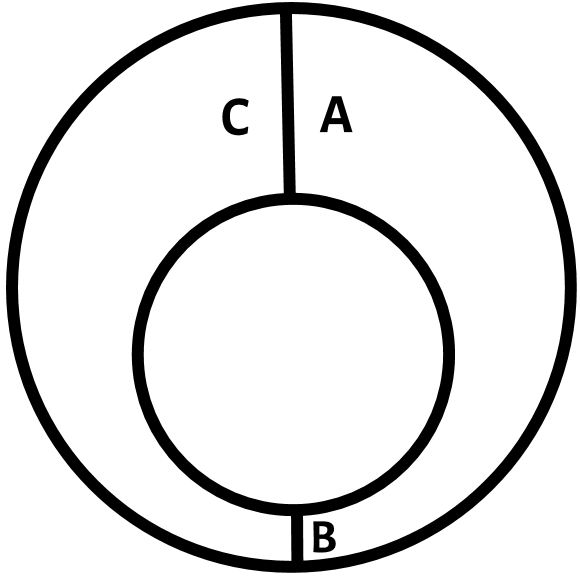
\includegraphics[width=1.25in,height=1.25in]{hegel-img002.png}
\end{center}}, "--- <<Математики>>, говорит он:
<<умозаключают, что неравенства, возможные в таком пространстве, бесконечны
не от бесконечного {\em множества} частей, ибо
{\em величина} этого пространства является {\em определенной} и
{\em ограниченной} и я могу предположить такое
пространство б\'{о}льшим или меньшим, а они делают этот вывод на том
основании, что {\em природа этой вещи} превосходит всякую
определенность>>\pagenote{Гегель дает здесь
в весьма вольном переводе и с перестановкой отдельных предложений
рассуждения Спинозы о бесконечном множестве неравных расстояний между двумя
неконцентрическими окружностями (см. Спиноза, Переписка, М.~1932, стр.~78).
Конец приводимой Гегелем цитаты у Спинозы гласит: <<\ldots природа этой вещи
не~может быть выражена никаким числом>>.}. "--- Как видим, Спиноза
отвергает то представление о бесконечном, согласно которому представляют
себе его как множество или как незавершенный ряд, и напоминает, что в
пространстве, приводимом им как пример, бесконечное не находится по ту
сторону, а налично и полно; это пространство есть нечто ограниченное, но
бесконечное именно потому, <<что природа вещи превосходит всякую
определенность>>, так как содержащееся в нем определение величины вместе с
тем не может быть представлено как некоторое определенное количество или,
употребляя вышеприведенное выражение Канта,
{\em синтезирование} не может быть закончено, доведено
до некоторого "--- дискретного "--- определенного количества. "--- Каким образом
противоположность между {\em непрерывным} и
{\em дискретным} определенным количеством приводит к
бесконечному, "--- это мы разъясним в одном из следующих примечаний. "---
Бесконечное некоторого ряда Спиноза называет
{\em бесконечным воображения}, бесконечное же, как
соотношение с собою самим, он называет {\em бесконечным
мышления} или infinitum actu (актуально бесконечным). Оно именно actu,
{\em действительно} бесконечно, так как оно завершено
внутри себя и налично. Так например, ряд
$0{,}285714\ldots$ или $1+a+a^2+a^3\ldots$
есть лишь бесконечное воображение или мнения, ибо он не обладает
действительностью, ему безоговорочно чего-то недостает. Напротив,
$\frac 2 7$ или $\frac 1{1-a}$ есть в действительности не только то,
что ряд представляет собою в своих наличных членах, но вдобавок к этому
еще и то, чего ему недостает, чем он только {\em должен быть}.
$\frac 2 7$ или $\frac 1{1-a}$
есть такая же конечная величина, как заключенное между двумя
кругами пространство и его неравенства в примере Спинозы, и, подобно этому
пространству, она может быть сделана большей или меньшей. Но отсюда не
получается несообразность большего или меньшего бесконечного, так как это
определенное количество целого не касается отношения его моментов,
{\em природы вещи}, т.~е. качественного определения
величины; то, что в бесконечном ряде {\em имеется
налицо}, есть также некоторое конечное определенное количество, но кроме
того еще нечто недостаточное. "--- Напротив,
{\em воображение} не идет дальше определенного
количества как такового и не принимает во внимание качественного
соотношения, составляющего основание имеющейся несоизмеримости.

Несоизмеримость, имеющая место в примере, приводимом Спинозой, заключает в
себе вообще криволинейные функции и приводит к тому бесконечному, которое
ввела математика при действиях с этими функциями и вообще при действиях
{\em с функциями переменных величин;} последнее есть
именно то {\em истинно математическое}, качественное
бесконечное, которое мыслил также и Спиноза. Это определение мы должны
здесь рассмотреть ближе.

Что касается, прежде всего, признаваемой столь важной категории
{\em переменности}, под которую подводятся соотносимые
в этих функциях величины, то они ближайшим образом переменны не в том
смысле, в котором в дроби $\frac 2 7$ переменны оба числа 2 и 7,
поскольку вместо них можно поставить также 4 и 14, 6 и 21 и~т.~д. до
бесконечности без изменения значения дроби. В~этом смысле можно еще с
большим правом поставить в дроби $\frac a b$ вместо
$a$ и $b$ любые числа без
изменения того, что должно выражать собою $\frac a b$.
Лишь в том смысле, что также и вместо $x$ и
$y$ в какой-либо функции можно поставить
бесконечное, т.~е. неисчерпаемое {\em множество} чисел,
$a$ и $b$ суть такие же
переменные величины, как и $x$ и
$y$. Поэтому выражение
<<{\em переменные величины}>> страдает неясностью и
неудачно выбрано для определений величин, интересность которых и способы
действий над которыми коренятся {\em в чем-то
совершенно другом}, чем только в их переменности.

Чтобы сделать ясным, в чем заключается истинное определение тех моментов
какой-нибудь функции, которыми занимается высший анализ, мы должны снова
вкратце обозреть указанные выше ступени. В~дробях $\frac 2 7$ или
$\frac a b$ числа 2 и 7, каждое само по себе, суть определенные
количества и соотношение для них несущественно; $a$ и
$b$ также должны быть представителями таких
определенных количеств, которые остаются тем, чт\'{о} они суть, также и вне
отношения. Далее, $\frac 2 7$ и $\frac a b$ суть также некоторые
постоянные определенные количества, некоторые частные; отношение составляет
некоторую численность, единицей которой служит знаменатель, а численностью
этих единиц "--- числитель или обратно. Если бы мы подставили вместо 2 и 7
"--- 4 и 14 и~т.~д., то отношение осталось бы тем же самым также и как
определенное количество. Но это существенно изменяется, например, в функции
$\frac{y^2} x=p$; здесь, правда, $x$ и
$y$ имеют значение определенных количеств; но
определенное частное имеют не $x$ и
$y$, а лишь $x$ и
$y^{2}$. Благодаря этому указанные
{\em члены} отношения $x$ и
$y$ не только не суть,
{\em во-первых}, такие-то определенные количества, но
и, {\em во-вторых}, их
{\em отношение} не есть некоторое постоянное
определенное количество (а также и не {\em имеется в
виду} таковое, как это, например, имеет место при
$a$ и $b$), не есть
постоянное частное, а это частное {\em как определенное
количество} совершенно {\em переменно}. Но это зависит
только от того, что $x$ находится в отношении не к
$y$, а к {\em квадрату}
$y$. Отношение некоторой величины к
{\em степени} есть не
{\em определенное количество}, а по существу
{\em качественное} отношение.
{\em Степенн\'{о}е отношение} есть
{\em то обстоятельство}, которое должно рассматриваться
как {\em основное определение}. "--- В функции же прямой
линии $y=ax$ выражение $\frac y x=a$ есть обыкновенная дробь и
частное; эта функция есть поэтому лишь {\em формально}
функция переменных величин или, иначе говоря, $x$ и
$y$ представляют собою здесь то же самое, что $a$ и $b$ в
$\frac a b$, они не имеют того определения, под которым их рассматривает
дифференциальное и интегральное исчисление. "--- Вследствие
{\em особенной} природы переменных величин в этом
способе рассмотрения было бы целесообразно ввести для них как особое
название, так и {\em особые обозначения}, отличные от
обычных названий и обозначений {\em неизвестных
величин} в каждом конечном, определенном ли или неопределенном уравнении, "---
это было бы указанием их существенного отличия от таких просто неизвестных
величин, которые в себе суть вполне определенные количества или
определенная совокупность определенных количеств. "--- И в самом деле, лишь
отсутствие сознания своеобразия того, что составляет интерес высшего
анализа и чем вызваны потребность в дифференциальном исчислении и
изобретение его, привело к включению функций первой степени, каково
уравнение прямой линии, в состав этого особого исчисления; доля вины за
такой формализм ложится также и на то недоразумение, по которому полагают,
что возможно выполнить само по себе правильное требование
{\em обобщения} какого-нибудь метода тем, что
опускается та {\em специфическая} определенность, на
которой основана потребность в этом методе, так что считается, что дело
идет в рассматриваемой нами области только о
{\em переменных величинах вообще}. Значительная доля
формализма в рассмотрении, равно как и трактовке этих предметов, несомненно
не имела бы места, если бы поняли, что дифференциальное исчисление касается
не переменных величин как таковых, а {\em степенных
определений}.

Но имеется еще дальнейшая ступень, на которой выступает в своем своеобразии
математическое бесконечное. В~уравнении, в котором
$x$ и $y$ положены
ближайшим образом как определенные некоторым степенным отношением,
$x$ и $y$ как таковые
должны еще означать некоторые определенные количества; и вот это значение
совершенно утрачивается в так называемых
{\em бесконечно малых разностях}.
$dx$, $dy$ уже не суть
определенные количества и не должны обозначать таковых, а имеют значение
лишь в своем соотношении, {\em имеют смысл лишь как
моменты}. Они уже больше не {\em нечто}, если
принимать нечто за определенное количество, не конечные разности; но
они и {\em не ничто}, не лишенный определения нуль. Вне
своего отношения они "--- чистые нули, но их следует брать только как моменты
отношения, как {\em определения} дифференциального
коэффициента $\frac{dx}{dy}$.

В этом понятии бесконечного определенное количество подлинно завершено в
некоторое качественное наличное бытие; оно положено как действительно
бесконечное; оно снято не только как то или иное определенное количество, а
как определенное количество вообще. Но при этом
{\em сохраняется количественная определенность} как
{\em элемент} определенных количеств, как принцип или,
как также выражались, она сохраняется {\em в своем
первом понятии}.

Против этого понятия и направлено все то нападение, которому подверглось
основное определение математики этого бесконечного, "--- дифференциального и
интегрального исчисления. Неправильные представления самих математиков
вызвали непризнание этого понятия; но преимущественно вина за эти нападки
ложится на неспособность оправдать этот предмет как
{\em понятие}. Но понятия, как было указано выше,
математика не может здесь обойти, ибо как математика бесконечного она не
ограничивается рассмотрением {\em конечной}
определенности своих предметов, "--- как, например, в чистой математике
пространство и число и их определения рассматриваются и соотносятся друг с
другом лишь со стороны их конечности, "--- а она приводит заимствованное
оттуда и рассматриваемое ею определение в
{\em тождество с его противоположностью}, превращая,
например, кривую линию в прямую, круг в многоугольник и~т.~д. Поэтому
действия, к которым она позволяет себе прибегать в дифференциальном и
интегральном исчислении, находятся в полном противоречии с природой
исключительно только конечных определений и их соотношений и, стало быть,
могли бы найти свое оправдание только в {\em понятии}.

Если математика бесконечного настаивала на том, что эти количественные
определения суть исчезающие величины, т.~е. такие величины, которые уже
больше не суть какие-либо определенные количества, но не суть также и
ничто, а еще представляют собою известную
{\em определенность относительно другого}, то
нападавшим на нее казалось, что ничего нет яснее того, что не может быть
такого, как они выражались, {\em среднего состояния}
между бытием и ничто. "--- Каково значение этого возражения и так называемого
среднего состояния, это уже было указано выше при рассмотрении категории
становления, примечание 4. Конечно, единство бытия и ничто не есть
{\em состояние;} состояние было бы таким определением
бытия и ничто, в которое эти моменты, так сказать, попали только случайно,
как бы впав в болезнь или подвергшись внешнему воздействию со стороны
ошибочного мышления, между тем как эта средина и это единство, исчезание,
которое есть также и становление, напротив, единственно и есть их
{\em истина}.

То, что бесконечно, говорили далее, не {\em подлежит
сравнению} как большее или меньшее; поэтому, не может быть отношения
бесконечного к бесконечному, по порядкам или достоинствам бесконечного, а
между тем мы встречаем таковые различия бесконечных разностей в науке,
трактующей о них. "--- В основании этого уже упомянутого выше возражения все
еще лежит то представление, что здесь идет речь об
{\em определенных количествах}, сравниваемых как
определенные количества, и что определения, которые уже не суть
определенные количества, не имеют больше никакого отношения друг к другу.
В~действительности же дело обстоит наоборот: то, что
{\em только} находится в отношении, не есть
определенное количество. Определенное количество есть такое определение,
которое вне своего отношения должно иметь совершенно безразличное к другим
наличное бытие, определение, которому должно быть безразлично его отличие
от некоего другого, между тем как качественное есть, напротив, лишь то, что
оно есть в своем различии от другого. Поэтому указанные бесконечные
величины не только сравнимы, но имеют бытие лишь как моменты сравнения,
отношения.

Я приведу важнейшие определения, которые были даны в математике относительно
этого бесконечного; из них сделается ясным, что в их основании лежит такая
мысль о предмете, которая согласуется с развитым здесь понятием, но что
создатели этой отрасли математики не обосновали этой мысли как понятие, и в
применениях они вынуждены были прибегать к обходным средствам,
противоречащим их лучшему делу.

Эта мысль не может быть определена правильнее, чем то сделал
{\em Ньютон}. Я~оставлю здесь в стороне определения,
принадлежащие к представлению движения и скорости (от которых он главным
образом и заимствовал название {\em флюксий}), так как
в них мысль выступает не с надлежащею абстрактностью, а конкретно, смешана
с формами, лежащими вне существа дела. Эти флюксии объясняются Ньютоном в
том смысле
(Princ. mathem. phil. nat., lib.~I, Lemma~XI, Schol.),
что он понимает под ними не
{\em неделимые} "--- форма, которою пользовались более
ранние математики, Кавальери и другие, и которая содержит в себе понятие
{\em само по себе} определенного количества, "--- а
{\em исчезающие делимые}. Он объясняет далее, что он
понимает под ними не суммы и отношения определенных частей, а
{\em пределы} (limites) {\em сумм}
и {\em отношений}. Против этого выдвигают, дескать, то
возражение, что у исчезающих величин не может быть никакого
{\em последнего отношения}, так как прежде, чем они
исчезли, оно не последнее, а когда они исчезли, нет никакого отношения. Но
под отношением исчезающих величин, указывает Ньютон, следует понимать не то
отношение, которое имеет место {\em до} или
{\em после} их исчезновения, а то отношение,
{\em вместе с которым} они исчезают (quacum
evanescunt). Точно так же {\em первое} отношение
возникающих величин есть то отношение, {\em вместе с
которым} они возникают.

В соответствии с состоянием научного метода того времени давалось лишь
объяснение, что под таким-то выражением следует понимать то-то. Но
заявление, что под таким-то выражением следует понимать то-то, есть,
собственно говоря, лишь субъективное предложение или же историческое
требование, причем не показывают, что такое понятие само по себе необходимо
и обладает внутренней истинностью. Но вышеизложенное показывает, что
выставленное Ньютоном понятие соответствует тому, как в предшествующем
изложении получилась бесконечная величина из рефлексии определенного
количества внутрь себя. Под флюксиями Ньютон понимает величины в их
исчезновении, т.~е. величины, которые уже больше не суть определенные
количества; он, далее, понимает под ними не отношения определенных частей,
а {\em пределы отношения}. Стало быть, исчезают
согласно этому пониманию как определенные количества сами по себе, члены
отношения, так и самое отношение, поскольку оно было определенным
количеством, предел отношения величин есть то, в чем оно есть и не есть;
это означает, точнее, что оно есть то, в чем определенное количество
исчезло, и тем самым сохранились лишь отношение как качественно
количественное отношение, и его члены "--- тоже как качественно количественные
моменты. "--- Ньютон к этому прибавляет, что из того обстоятельства, что
существуют последние отношения исчезающих величин, не следует заключать,
что существуют последние, величины <<{\em неделимые}>>.
Это было бы опять-таки скачком от абстрактного отношения к таким его
членам, которые должны были бы сами по себе, вне своего соотношения, иметь
известное значение, как неделимые, как нечто, что было бы одним,
безотносительным.

Чтобы предостеречь против этого недоразумения, он, кроме того, напоминает,
что {\em последние отношения} суть не отношения
{\em последних величин}, а только пределы, к которым
{\em отношения} безгранично убывающих величин
приближаются больше, чем всякая {\em данная}, т.~е.
конечная разность, но которых они не преступают, чтобы стать ничем. "--- Под
{\em последними величинами} можно было бы именно
понимать, как мы уже сказали, неделимые или одни. Но из определения
последнего отношения устранено представление как о безразличном
безотносительном одном, так и о конечном определенном количестве. "--- Но не
нужно было бы ни {\em безграничного убывания}, которое
Ньютон приписывает определенному количеству и которое лишь служит
выражением бесконечного прогресса, ни определения делимости, которое здесь
уже больше не имеет никакого непосредственного значения, если бы требуемое
определение было развито далее в понятие некоторого такого определения
величины, которое есть исключительно лишь момент отношения.

Касательно {\em сохранения отношения} в
{\em исчезающих определенных количествах} мы встречаем
у других авторов (например, у {\em Карно},
Réflexions sur la métaphysique du Calcul infinitésimal)
выражение, что {\em в силу закона непрерывности}
исчезающие величины прежде, чем исчезнуть, продолжают
сохранять то отношение, из которого они происходят. "--- Это представление
{\em выражает} собою истинную природу дела, поскольку
здесь разумеется не та непрерывность определенного количества, которую оно
являет нам в бесконечном прогрессе, непрерывность, заключающаяся в том, что
определенное количество так продолжается в своем исчезновении, что
{\em по ту сторону} его снова возникает лишь некоторое
конечное определенное количество, некоторый {\em новый
член ряда}. Однако {\em непрерывное} движение вперед
всегда представляют себе так, что проходятся значения, которые еще суть
конечные определенные количества. Напротив, в том переходе, который
совершается в истинное бесконечное, {\em непрерывным}
оказывается отношение; оно настолько {\em непрерывно} и
сохраняется, что переход исключительно только и состоит в том, что он
выделяет отношение в чистом виде и заставляет исчезнуть безотносительное
определение, т.~е. то обстоятельство, что определенное количество,
являющееся членом отношения, еще есть определенное количество также и
тогда, когда оно положено вне этого соотношения. "--- Это очищение
количественного отношения есть постольку не что иное, как то, что имеет
место, когда некоторое эмпирическое {\em существование}
(Dasein) постигается через {\em понятие} (begriffen
wird). Эмпирическое существование благодаря этому поднимается выше самого
себя таким образом, что его понятие содержит те же определения, которые
содержит оно само, но охваченные в их существенности и вдвинутые в
{\em единство} понятия, в котором они потеряли свое
безразличное, чуждое понятию существование (Bestehen).

Столь же интересна и другая форма ньютоновой трактовки интересующих нас
величин, а именно, рассмотрение их как
{\em производящих величин} или
{\em начал}. {\em Производная}
величина (genita) "--- это произведение или частное, корни, прямоугольники,
квадраты, а также стороны прямоугольников, квадратов, "--- вообще,
{\em конечная величина}. "--- <<Рассматривая ее как
переменную, как возрастающую или убывающую в постоянном движении и течении,
я понимаю под названием {\em моментов} ее
{\em моментальные приращения} или
{\em убывания}. Но не следует принимать эти моменты за
частицы, имеющие определенную величину (particulae finitae). Такие частицы
суть не самые {\em моменты}, а величины,
{\em произведенные} из моментов; под последними же
следует понимать находящиеся в становлении
{\em принципы} или {\em начала}
конечных величин>>. "--- Ньютон отличает здесь определенное количество от него
же самого, рассматривает его двояко: так, как оно есть продукт или налично
сущее, и так, как оно есть в своем {\em становлении}, в
своем {\em начале} и
{\em принципе}, то есть как оно есть в своем
{\em понятии} или "--- здесь это равнозначно "--- в своем
качественном определении; в последнем количественные различия, бесконечные
приращения или убывания суть лишь моменты; только уже ставшее есть нечто
перешедшее в безразличие наличного бытия и во внешность, "--- определенное
количество. "--- Но если философия истинного понятия и должна признать эти
приведенные касательно приращений или убываний определения бесконечного, то
мы должны вместе с тем сразу же заметить, что самые формы приращения
и~т.~д. имеют место {\em внутри} категории
непосредственного определенного количества и вышеуказанного непрерывного
движения вперед, и что представления о
{\em приращении}, {\em приросте},
увеличении {\em x} на {\em dx} или
{\em i} и~т.~д. должны рассматриваться скорее как
имеющиеся в этих методах основные недостатки, как постоянное препятствие к
выделению в чистом виде определения качественного момента количества из
представления об обычном определенном количестве.

По сравнению с указанными определениями является очень отсталым
{\em представление о бесконечно-малых величинах},
содержащееся также и в самих представлениях о приращении или убывании.
Согласно представлению о бесконечно-малых величинах они носят такой
характер, что следует {\em пренебрегать} не только ими
самими по отношению к конечным величинам, но также их высшими порядками по
отношению к низшим, а равно произведениями нескольких таких величин по
отношению к одной. "--- У {\em Лейбница} особенно ярко
выступает это требование о таком {\em пренебрежении},
применению какового давали место также и предыдущие изобретатели методов,
касающихся этих величин. Именно это обстоятельство сообщает указанному
исчислению при всем выигрыше в удобстве видимость неточности и явной
неправильности хода его действий. "--- {\em Вольф}
стремился сделать это пренебрежение величинами понятными по обычному своему
способу делать популярными излагаемые им вопросы, т.~е. путем нарушения
чистоты понятия и подстановки на его место неправильных чувственных
представлений. А~именно, он сравнивает пренебрежение бесконечно малыми
разностями высших порядков относительно низших с образом действия геометра,
измерение которым высоты горы нисколько не делается менее точным, если
ветер снесет песчинку с ее вершины, или с пренебрежением высотой домов и
башен при вычислении лунных затмений (Element. Mathes. univ.,
Tom~I, El. Analys. math., P.~II, С~I, см.~Schol.).

Если снисходительная справедливость (die Billigkeit) здравого человеческого
рассудка и допускает такую неточность, то все геометры, напротив, отвергали
такого рода представление. Сама собою напрашивается мысль, что в
математической науке не идет речь о такой эмпирической точности и что
математическое измерение путем ли вычислений или путем геометрических
построений и доказательств совершенно отлично от землемерия, от измерения
данных в опыте линий, фигур и~т.~п. Да и помимо того, как уже было указано
выше, аналитики, сравнивая между собою результаты, получаемые строго
геометрическим путем, с результатами, получаемыми посредством метода
бесконечно малых разностей, доказывают, что они тождественны и что большая
или меньшая точность здесь вовсе не имеет места. А~ведь само собою понятно,
что абсолютно точный результат не мог бы получиться из неточного хода
действия. Однако, с другой стороны, несмотря на протесты против этого
способа оправдания, никак нельзя обойтись без
{\em самого этого приема} "--- без пренебрежения величиной
на основании ее незначительности. И~в этом состоит трудность, заставляющая
аналитиков стараться сделать понятным и устранить заключающуюся здесь
бессмыслицу.

По этому вопросу следует главным образом привести мнение
{\em Эйлера}. Полагая в основание общее определение
Ньютона, он настаивает на том, что дифференциальное исчисление рассматривает
{\em отношения приращений} некоторой величины, причем,
однако, {\em бесконечно малая разность} как таковая
должна быть рассматриваема совершенно {\em как нуль}
(Institut Calc. different., р.~I, с.~III).
"--- Как это следует понимать, видно из
вышеизложенного; бесконечно малая разность есть нуль лишь по количеству, а
не качественный нуль; а как нуль по количеству, она есть лишь чистый момент
отношения. Она не есть различие {\em на некоторую
величину}. Но именно потому, с одной стороны, вообще ошибочно называть
моменты, именуемые бесконечно малыми величинами, также и приращениями или
убываниями и {\em разностями}. В~основании этого
определения лежит предположение, что к первоначально имеющейся конечной
величине нечто {\em прибавляется} или нечто от нее
{\em отнимается}, что совершается некоторое вычитание
или сложение, некоторое {\em арифметическое},
{\em внешнее} действие. Но что касается перехода от
функции переменной величины к ее дифференциалу, то по нему видно, что он
носит совершенно другой характер, а именно, как мы уже разъяснили, он
должен рассматриваться как сведение конечной функции к качественному
отношению ее количественных определений. "--- С другой стороны, сразу
бросается в глаза, что когда говорят, что приращения суть сами по себе нули
и что рассматриваются лишь их отношения, то это само по себе ошибочно, ибо
нуль уже не имеет вообще никакой определенности. Это представление, стало
быть, хотя и доходит до отрицания количества и определенно высказывает это
отрицание, не схватывает вместе с тем последнего в его положительном
значении качественных определений количества, которые, если пожелаем
вырвать их из отношения и брать их как определенные количества, окажутся
лишь нулями. "--- {\em Лагранж} (Théorie des fonct. analyt. Introd.)
замечает о представлении {\em пределов} или {\em последних
отношений}, что, хотя и можно очень хорошо представить себе отношение двух
величин, покуда они остаются конечными, это отношение не дает рассудку
ясного и определенного понятия, как только его члены становятся
одновременно нулями. "--- И в самом деле, рассудок должен пойти далее той
чисто отрицательной стороны, что члены отношения суть как определенные
количества нули, и понять их положительно как качественные моменты. "--- А то,
что {\em Эйлер} (в указанном месте \S~84 и~сл.)
прибавляет далее касательно данного им определения, чтобы показать, что две
так называемые бесконечно малые величины, которые якобы суть не что иное,
как нули, тем не менее находятся в отношении друг к другу, и потому для их
обозначения употребляется не знак нуля, а другие знаки, "--- не может быть
признано удовлетворительным. Он хочет это обосновать различием между
арифметическим и геометрическим отношениями; в первом мы обращаем внимание
на разность, во втором "--- на частное, и, хотя арифметическое отношение между
любыми двумя нулями всегда одинаково, это не значит, что можно сказать то
же самое о геометрическом отношении; если $2 : 1 = 0 : 0$,
то по свойству пропорции, так как первый член вдвое больше второго, третий
член тоже должен быть вдвое больше четвертого; поэтому на основании этой
пропорции отношение $0 : 0$ должно быть взято, как отношение
$2 : 1$. "--- Также и по обычной арифметике $n \times 0 = 0$; следовательно,
$n : 1 = 0 : 0$. "--- Однако именно потому, что $2 : 1$ или $n : 1$
есть отношение определенных количеств, ему не соответствует ни отношение,
ни обозначение $0 : 0$.

Я воздерживаюсь от дальнейшего увеличения числа приведенных взглядов, так
как рассмотренные уже достаточно показали, что в них, правда, скрыто
содержится истинное понятие бесконечного, но что оно, однако, не выделено и
не сформулировано во всей его определенности. Поэтому, когда высказывающие
эти взгляды переходят к самому действию, то на нем не может сказаться
истинное определение понятия, а, напротив, возвращается снова конечная
определенность количества, и действие не может обойтись без представления о
лишь {\em относительно малом}. Исчисление делает
необходимым подвергать так называемые бесконечные величины обычным
арифметическим действиям сложения и~т.~д., основанным на природе конечных
величин, и тем самым хотя бы на мгновение признавать эти бесконечные
величины конечными и трактовать их как таковые. Исчисление должно было бы
обосновать правомерность того, что оно, с одной стороны, тянет эти величины
вниз, вовлекает их в эту сферу и трактует их как приращения или разности, а
с другой стороны, пренебрегает ими как определенными количествами после
того, как оно только что применяло к ним формы и законы конечных величин.

Я приведу еще самое существенное о попытках геометров устранить эти
затруднения.

Более старые аналитики меньше затрудняли себя такими сомнениями; но старания
более новых аналитиков были направлены преимущественно к тому, чтобы
возвратить исчисление бесконечно малых к очевидности
{\em собственно геометрического метода} и с помощью
этого метода достигнуть в математике {\em строгости
доказательств древних} (выражения {\em Лагранжа}).
Однако, так как принцип анализа бесконечного по своей природе выше, чем
принцип математики конечных величин, то анализ бесконечного сам собою сразу
же должен был отказаться от того рода
{\em очевидности}, подобно тому, как философия также не
может притязать на ту отчетливость, которой обладают науки о чувственном,
например, естественная история, или подобно тому, как еда и питье считаются
более понятными вещами, чем мышление и постижение посредством понятия
(Begreifen). Поэтому нам придется говорить лишь о стараниях достигнуть
строгости доказательств древних.

Некоторые математики пытались обойтись совершенно без понятия бесконечного и
дать без него то, чт\'{о} казалось связанным с его употреблением. "---
{\em Лагранж}, например, рассказывает о методе,
изобретенном {\em Ланденом}, и говорит о нем, что он
является чисто аналитическим и не употребляет бесконечно малых разностей, а
сначала вводит {\em различные значения} переменных
величин и в дальнейшем {\em приравнивает} их между
собою. Лагранж, впрочем, заявляет, что в этом методе утрачиваются
свойственные дифференциальному исчислению преимущества, а именно простота
метода и легкость действия. "--- Это "--- прием, в котором есть нечто
соответственно тому, из которого исходит {\em Декартов}
метод касательных, о котором нам придется ниже еще говорить подробнее.
Здесь можем заметить, что в общем виде сразу ясно, что этот прием,
заключающийся в том, чтобы придавать переменным величинам различные
значения и затем приравнивать их между собою, принадлежит вообще к другому
кругу математической трактовки, чем сам метод дифференциального исчисления,
и им не выделяется подлежащее далее более пристальному рассмотрению
своеобразие того простого отношения, к которому сводится действительное,
конкретное определение этого исчисления, а именно "--- отношения производной
функции к первоначальной.

Более ранние из новых математиков, как например,
{\em Ферма}, {\em Барроу} и др.,
которые впервые пользуются бесконечно малыми в том применении, которое
позднее привело к разработке дифференциального и интегрального исчисления, а
затем также {\em Лейбниц} и последующие математики,
равно как и {\em Эйлер}, всегда откровенно
высказывались, что считают дозволительным отбрасывать произведения
бесконечно малых разностей так же, как и их высшие степени только на том
основании, что они {\em относительно}, по сравнению с
низшими порядками, {\em исчезают}. Исключительно на
этом соображении покоится у них {\em основная теорема},
а именно, определение того, что такое дифференциал произведения или степени,
{\em ибо }{\em к этому сводится все
теоретическое учение}. Остальное есть отчасти механизм действий, отчасти же
приложение, которое, однако, как мы покажем далее, на самом деле
представляет более высокий или, лучше сказать, единственный интерес. "---
Относительно же того вопроса, который мы рассматриваем теперь, следует
здесь привести лишь то элементарное соображение, что на основании того же
рассуждения о {\em незначительности} принимается как
основная теорема о кривых, что элементы кривых, а именно
{\em приращения} абсциссы и ординаты имеют между собою
то же {\em отношение}, как
{\em подкасательная} и
{\em ордината}. С~целью получить подобные треугольники
дуга, составляющая наряду с двумя приращениями третью сторону того
треугольника, который справедливо назывался когда-то
{\em характеристическим} треугольником, рассматривается
как прямая линия, как часть касательной, и потому одно из приращений "--- как
доходящее до касательной. Эти допущения поднимают, с одной стороны,
вышеуказанные определения выше природы конечных величин; но, с другой
стороны, здесь применяется к моментам, называемым теперь бесконечными,
такой прием, который значим лишь относительно конечных величин и при
котором мы не имеем права чем-либо пренебрегать на основании его
незначительности. Затруднение, тяготеющее над методом, остается при таком
образе действия во всей своей силе.

Здесь мы должны указать на замечательный прием {\em Ньютона}
(Princ. Mathem. phil. nat., lib.~II, Lemma~II, после propos.~VII)
"--- на изобретенный им остроумный кунштюк для устранения арифметически
неправильного отбрасывания произведений бесконечно малых разностей или
высших порядков этих последних при нахождении дифференциалов. Он находит
дифференциал произведения, "--- из которого легко затем вывести дифференциалы
частного, степени и~т.~п. "--- следующим образом. Произведение, если уменьшить
$x$ и $y$, каждый порознь
{\em на половину} его бесконечной разности, переходит в
$xy - \frac {xdy} 2 - \frac {ydx} 2 + \frac {dxdy} 4$,
а если увеличить $x$ и $y$ ровно настолько же, то произведение
переходит в $xy + \frac {xdy} 2 + \frac {ydx} 2 + \frac {dxdy} 4$.
Если от этого второго произведения отнять первое, то получается
разность $ydx + xdy$, которая есть {\em избыток приращения на целые}
$dx$ и $dy$, так как на это
приращение отличаются оба произведения; следовательно, это и есть
дифференциал $xy$. "--- Как видим, при этом приеме сам собою
отпадает член, представлявший главное затруднение, произведение двух
бесконечных разностей $dxdy$. Но, несмотря на имя
{\em Ньютона}, следует сказать, что это, хотя и весьма
элементарное, действие неправильно; неправильно, что
$\left(x+\frac{dx} 2\right)\left(y+\frac{dy}
2\right)-\left(x-\frac{dx} 2\right)\left(y-\frac{dy}
2\right)=\left(x+dx\right)\left(y+dy\right)-xy$.

Только потребность обосновать ввиду его важности исчисление флюксий могла
заставить такого математика, как Ньютон, обмануть себя подобным способом
доказательства.

Другие формы, которыми пользуется Ньютон при выводе дифференциала, связаны с
конкретными, относящимися к движению значениями элементов и их степеней. "---
При употреблении {\em формы ряда}, которое вообще
характерно для его метода, слишком напрашивается сказать, что мы всегда
имеем возможность путем прибавления дальнейших членов взять величину
{\em с той степенью точности},
{\em которая нам нужна}, и что отброшенные величины
{\em относительно незначительны}, что вообще результат
есть лишь {\em приближение;} и он здесь также
удовлетворился этим основанием, подобно тому, как он в своем методе решения
уравнений высших степеней путем приближения отбрасывает высшие степени,
получающиеся при подстановке в данное уравнение каждого найденного еще
неточного значения, на том же грубом основании, что они малы; см.
{\em Lagrange}, Equations Numériques, р.~125.

{\em Ошибка}, в которую впал
{\em Ньютон}, разрешая задачу путем отбрасывания
существенных высших степеней, ошибка, которая дала повод противникам
торжествовать победу своего метода над его методом и истинный источник
которой обнаружил {\em Лагранж} в своем новейшем ее рассмотрении
(Théorie des fonct. analyt., 3-me~р., ch.~IV),
доказывает, что употребление этого орудия еще страдало
{\em формализмом} и {\em неуверенностью}. {\em Лагранж}
показывает, что {\em Ньютон} впал в свою ошибку
вследствие того, что он пренебрегал членом ряда, содержащим ту степень,
которая была важна для данной задачи. {\em Ньютон}
придерживался формального, поверхностного принципа отбрасывания членов
ввиду их относительной малости. "--- А именно, известно, что в
{\em механике} членам ряда, в который разлагается
функция какого-нибудь движения, придается
{\em определенное значение}, так что первый член или
первая функция относится к моменту скорости, вторая "--- к силе ускорения, а
третья "--- к сопротивлению сил. Поэтому члены ряда должны рассматриваться
здесь не только как {\em части} некоторой суммы, но как
{\em качественные моменты некоторого целостного
понятия}. Благодаря этому {\em отбрасывание} остальных
членов, принадлежащих дурно бесконечному ряду, имеет
{\em смысл}, совершенно
{\em отличный} от отбрасывания их на основании их
относительной малости\footnote{Обе точки зрения весьма просто
сопоставлены у Лагранжа при
применении теории функций в механике, в главе о прямолинейном движении
(Théorie des fonct. 3-me~р., ch.~I, art.~IV). Если
рассматривать пройденное пространство как функцию протекшего времени, то
получается уравнение $x=ft$, которое, разложенное
как $f(t+\vartheta )$, даёт
$ft + \vartheta f't + \frac{\vartheta ^{'2}} 2 f''t + $
и~т.~д. Следовательно, пространство, пройденное в данное время,
изображается формулой
$ = \vartheta f't+\frac{\vartheta ^2}
2 f''t + \frac{\vartheta ^3}{2 \cdot 3} f'''t + $
и~т.~д. Движение, посредством которого проходится это
пространство, говорят нам, {\em составлено}, {\em следовательно} (т.~е.
вследствие того, что аналитическое разложение в ряд дает много и притом
бесконечно много членов) "--- из различных частичных движений,
соответствующие времени пространства которых суть
$ \vartheta f't+\frac{\vartheta ^2}
2 f''t + \frac{\vartheta ^3}{2 \cdot 3} f'''t + $
и~т.~д. Первое частичное
движение есть в известном нам движении формально-равномерное движение со
скоростью $f't$, второе равномерно ускоренное, зависящее
от силы ускорения, пропорциональной $f^{\text{[2033?]}}t$.
<<А так как прочие члены не {\em относятся ни к какому простому
известному движению, то нет надобности принимать} их в
отдельности {\em во внимание}, и мы покажем, что
{\em от них можно абстрагироваться} при определении движения в
начале момента времени>>. Это и показывается, но, конечно, только путём
{\em сравнения} вышеуказанного ряда, члены которого {\em все} должны были
служить для определения {\em величины}
пространства, пройденного в данное время, с данным в \S~3 для
падения тел уравнением $x=at+bt^2$, в
котором имеются только эти два члена. Но это уравнение само получило этот
вид лишь благодаря предположению {\em объяснения}, {\em даваемого} членам,
возникающим {\em посредством аналитического разложения в ряд},
это предположение заключается в том, что равномерно ускоренное движение
{\em составлено} из формально равномерного движения, совершающегося
с достигнутой в предыдущую часть времени скоростью, и некоторого прибавка
($a$ в уравнении $s=at^2$), т.~е. эмпирического коэффициента,
приписываемого силе тяжести, а ведь это есть такое различение, которое
отнюдь не имеет существования или основания в природе вещей, но есть лишь
ошибочно получившее характер физического положения выражение того, что
получается при принятии некоторой определенной аналитической трактовки.}.
Разрешение проблемы, данное Ньютоном, оказалось ошибочным не потому, что в
нем не принимаются во внимание члены ряда лишь как
{\em части некоторой суммы}, а потому, что не
принимается во внимание {\em член, содержащий то
качественное определение}, в котором было все дело.

В этом примере качественный {\em смысл} есть то, от чего
ставится в зависимость прием. В~связи с этим мы можем тотчас же выставить
общее утверждение, что все затруднение касательно самого принципа было бы
устранено, если бы вместо формализма, состоящего в том, что определение
{\em дифференциала} усматривают лишь в дающей ему это
{\em имя} задаче, т.~е. в
{\em различии} вообще некоторой функции от ее
{\em изменения} после того, как ее переменная величина
получила некоторое {\em приращение}, "--- если бы вместо
этого формализма было указано качественное значение принципа и действие
было бы поставлено в зависимость от этого качественного значения. В~этом
смысле дифференциал от $x^n$ оказывается вполне исчерпанным первым членом
ряда, получающегося путем разложения выражения $(x+dx)^n$. Что
прочие члены не принимаются во внимание, проистекает, таким образом, не из
их относительной малости; здесь не предполагается никакой такой неточности,
погрешности или ошибки, которая бы {\em выравнивалась}
и {\em исправлялась} другой ошибкой, "--- взгляд, исходя
преимущественно из которого, {\em Карно} оправдывает
обычный метод исчисления бесконечно-малых. Так как дело идет
{\em не} о некоторой {\em сумме}, а
о некотором {\em отношении}, то дифференциал оказывается
вполне найденным {\em посредством первого члена;} там
же, где есть нужда в дальнейших членах, в дифференциалах высших порядков, их
нахождение состоит не в продолжении ряда, как
{\em суммы}, а в повторении одного и того же
{\em отношения}, которое единственно имеют в виду и
которое, стало быть, {\em завершено} уже в
{\em первом члене}. Потребность в
{\em форме} некоторого {\em ряда},
в суммировании этого ряда и все, что связано с этим, должны в таком случае
быть совершенно отделены от указанного {\em интереса к
отношению}.

Разъяснения, даваемые {\em Карно} относительно метода
бесконечных величин, представляют собою наиболее очищенное и ясное
изложение того, что нам встретилось в вышеуказанных представлениях. Но при
переходе к самим действиям у него более или менее появляются обычные
представления о бесконечной {\em малости} отбрасываемых
членов {\em по сравнению} с другими. Он оправдывает
метод скорее тем, что {\em результаты} оказываются
правильными, и {\em полезностью} введения
{\em неполных} уравнений, как он их называет (т.~е.
таких уравнений, в которых совершается такое арифметически неправильное
отбрасывание), для упрощения и сокращения исчисления, "--- чем самой природой
вещи.

{\em Лагранж}, как известно, снова возвратился к
первоначальному методу Ньютона, к методу рядов, дабы быть свободным от
трудностей, которые влечет за собою представление о бесконечно-малом, равно
как и метод первых и последних отношений и пределов. Относительно его
исчисления функций, прочие преимущества которого в отношении точности,
абстрактности и всеобщности достаточно известны, мы должны отметить как
касающееся занимающего нас вопроса лишь то, что оно покоится на той
основной теореме, что разность, не превращаясь в нуль,
{\em может быть принята столь малой, чтобы каждый член
ряда превосходил по своей величине сумму всех следующих за ним членов}. "---
При этом методе также начинают с категорий
{\em приращения} и {\em разности}
(по сравнению с первоначальной функцией) той функции, переменная величина
которой получает {\em приращение}, что и вызывает
появление скучного ряда; равно как в дальнейшем члены ряда, которые должны
быть отброшены, принимаются в соображение лишь с той стороны, что они
составляют некоторую {\em сумму}, и основанием, почему
они отбрасываются, полагается относительность их
{\em определенного количества}. Отбрасывание,
следовательно, и здесь не сводится в общем виде к той точке зрения, которая
отчасти встречается в некоторых приложениях, в которых, как мы упомянули
раньше, члены ряда должны иметь определенное
{\em качественное значение} и оставляются без внимания
не потому, что они незначительны по величине, а потому, что они
незначительны по качеству; отчасти же само отбрасывание отпадает в той
существенной точке зрения, которая определенно выступает относительно так
называемых дифференциальных коэффициентов лишь в так называемом
{\em приложении} дифференциального исчисления у
{\em Лагранжа}, что мы разъясним подробнее в следующем
примечании.

{\em Качественный характер вообще}, свойственный (как мы
здесь доказали, трактуя о той форме величины, о которой идет речь) тому,
что при этом называется бесконечно малым, обнаруживается непосредственнее
всего в той категории {\em предела отношения}, которая
приведена выше и проведение которой в дифференциальном исчислении
рассматривалось как некоторый особого рода метод. Из соображений в суждении
Лагранжа об этом методе, что ему недостает легкости применения и что
выражение <<{\em предел}>> не дает определенной идеи, мы
остановимся на втором и рассмотрим ближе аналитическое значение этого
метода. В~представлении о пределе именно и содержится вышеуказанная
истинная категория {\em качественного} определения
отношения между переменными величинами; ибо те их формы, которые появляются
в нем, {\em dx} и {\em dy}, должны
быть взяты здесь просто лишь как моменты выражения
$\frac{dy}{dx}$ и само
$\frac{dx}{dy}$ должно рассматриваться как единый
неделимый знак. Что при этом для механизма исчисления, особенно в его
приложении, утрачивается преимущество, которое он извлекает из того
обстоятельства, что члены дифференциального коэффициента отделяются друг от
друга, "--- это следует здесь оставить в стороне. Этот предел должен быть
теперь {\em пределом} некоторой данной функции; он
должен указать известное значение в связи с нею, определяемое способом
вывода. Но с голой категорией предела мы не подвинулись бы дальше, чем с
тем, о чем дело шло в этом примечании, имеющем целью показать, что
бесконечно-малое, выступающее в дифференциальном исчислении как
{\em dx} и {\em dy}, имеет не только отрицательный, пустой смысл некоторой
{\em не}-конечной, {\em не}-данной величины, как это имеет место,
например, в тех случаях, когда говорится: <<бесконечное множество>>, <<и~т.~д.
до бесконечности>> и~т.~п., а определенный смысл качественной определенности
количественного, момента отношения как такового. Однако эта категория,
взятая в таком смысле, еще не имеет отношения к тому, что есть некоторая
данная функция, еще не влияет сама по себе на трактовку этой функции и не
приводит к такому употреблению указанного определения, которое должно было
бы иметь место в последней; таким образом, и представление предела, если
этому представлению не дозволяют идти дальше такой доказанной относительно
него определенности, также ни к чему не привело бы. Но выражение <<предел>>
уже само по себе подразумевает, что он есть предел
{\em чего-то}, т.~е. выражает известное значение,
определяемое функцией переменной величины; и мы должны посмотреть, каков
характер этого конкретного оперирования им.

Он должен быть пределом {\em отношения} друг к другу тех
двух {\em приращений}, на которые по сделанному
допущению {\em увеличиваются} две переменные величины,
соединенные в одном уравнении, из коих одна рассматривается как функция
другой; приращение берется здесь вообще неопределенным, и постольку о
бесконечно-малом нет еще и речи. Но прежде всего путь, которым отыскивается
этот предел, приводит к тем же непоследовательностям, которые имеются в
других методах. Этот путь именно таков. Если $y=fx$, то при
переходе $y$ в $y+k$ $fx$
должна переходить в $fx+ph+qh^2+rh^3$ и~т.~д.
Следовательно, $k=ph+qh^2$ и~т.~д., и
$\frac k h = p + qh + rh^2$ и~т.~д. Если теперь $k$ и
$h$ исчезают, то исчезает и второй член ряда кроме
$p$, каковое $p$ и
оказывается пределом отношения этих двух приращений. Отсюда видно, что
$h$ как определенное количество полагается
$= 0$, но что вследствие
этого $\frac k h$ еще не обращается вместе с тем в $\frac 0 0$, а
остается некоторым отношением. И~вот представление
{\em предела} должно доставить ту выгоду, что оно
устранит заключающуюся в этом непоследовательность;
$p$ должно вместе с тем быть не действительным
отношением, которое было бы $=\frac 0 0$, а лишь тем определенным
значением, к которому отношение может {\em приближаться
бесконечно}, т.~е. так, чтобы {\em разность могла стать
меньше всякой данной разности}. Более определенный смысл
{\em приближения} касательно того, что собственно
должно сближаться между собою, будет рассмотрен ниже. "--- Но что
количественное различие, определяемое не только как
{\em могущее}, но и как
{\em долженствующее быть} менее всякой данной величины,
уже больше не есть количественное различие, это само собою ясно; это так же
очевидно, как только что-нибудь может быть очевидным в математике; но этим
мы не пошли дальше $\frac{dy}{dx}=\frac 0 0$. Напротив,
если $\frac{dy}{dx} = p$, т.~е. принимается за некоторое
определенное количественное отношение, как это и есть на самом деле, то,
наоборот, получается затруднение для предположения, что $h=0$,
предположения, единственно путем которого и получается $\frac k h = p$.
Если же согласиться, что $\frac k h = 0$ "--- и в самом деле,
раз $h=0$, то само собою $k$ также делается $=0$, ибо
приращение $k$ к $у$ имеет
место лишь при условии существования приращения
$h$, "--- то надо было бы спросить, что представляет
собою $p$, которое есть некоторое совершенно
определенное количественное значение. На этот вопрос сразу же получается
простой, сухой ответ, гласящий, что оно есть коэффициент, и нам указывают,
путем какого вывода он возникает, "--- известным определенным образом
выведенная первая производная функция некоторой первоначальной функции.
Если удовольствоваться этим ответом, как и в самом деле
{\em Лагранж по существу дела} удовольствовался им, то
общая теория науки дифференциального исчисления и непосредственно сама та
одна форма, которая называется {\em теорией пределов},
освободилась бы от приращений, а затем и от их бесконечной или какой угодно
малости, от трудности, состоящей в том, что кроме первого члена или,
вернее, лишь коэффициента первого члена, все остальные члены ряда, которые
неминуемо появляются благодаря введению этих приращений, снова устраняются;
да помимо этого она очистилась бы также и от всего связанного с этим
дальнейшего, от формальных категорий прежде всего бесконечного,
бесконечного приближения, а затем и от дальнейших здесь столь же пустых
категорий непрерывной величины\footnote{Категория
{\em непрерывной} или {\em текучей величины} появляется вместе с рассмотрением
{\em внешнего и эмпирического} изменения величин,
приведенных некоторым уравнением в такую
связь, что одна есть функция другой; но так как научным предметом
дифференциального исчисления служит известное (обыкновенно выражаемое через
дифференциальный коэффициент) {\em отношение}, каковая
определенность может быть названа также и {\em законом}, то для
этой специфической определенности простая непрерывность есть отчасти
чужеродный аспект, отчасти же во всяком случае абстрактная, а здесь"--- пустая
категория, так как ею ничего не выражается о законе непрерывности. "---
В какие формальные дефиниции при этом, кроме того, впадают,
показывает остроумное общее изложение моим уважаемым коллегой проф.
{\em Дирксеном} основных
определений, употребляемых для вывода дифференциального исчисления,
изложение, которое он дает в связи с критикой некоторых новых сочинений по
этой науке, помещенной в Jahrb.~f.~wissensch. Kritik, 1827, Nr.~153 и~сл.
Там на стр.~1251
дается даже такая дефиниция: <<Непрерывная величина, континуум, есть всякая
величина, которая мыслится нами находящейся в таком состоянии становления,
при котором последнее совершается не
{\em скачкообразно}, а путем {\em непрерываемого движения
вперед}>>. Но ведь это тавтология, повторение того, что есть
и самое {\em definitum}.} и всех еще других, которые
считается нужным ввести, как, например,
{\em стремление}, {\em становление}, {\em повод к изменению}.
Но в таком случае требовалось бы показать, какое еще
{\em значение} и {\em ценность}, т.~е. какую {\em связь} и какое
{\em употребление} для дальнейших математических целей
имеет $p$ помимо того, для теории совершенно
достаточного сухого определения, что оно есть не что иное, как полученная
путем разложения бинома производная функция; об этом будет сказано во
{\em втором примечании}. "--- Здесь же мы ближайшим
образом дадим разбор той путаницы, которую вышеприведенное столь обычное в
изложениях употребление представления о
{\em приближении} внесло в понимание собственной,
качественной определенности того отношения, в котором было ближайшим
образом все дело.

Мы показали, что так называемые бесконечно малые разности выражают собою
исчезание членов отношения как определенных количеств и что то, что после
этого остается, есть их количественное отношение, исключительно лишь
поскольку оно определено качественным образом; качественное отношение здесь
настолько не теряется, что оно скорее есть именно то, что получается
благодаря превращению конечных величин в бесконечные. В~этом, как мы
видели, состоит вся суть дела. "--- Так например, {\em в
последнем отношении} исчезает определенные количества абсциссы и ординаты.
Но члены этого отношения остаются по существу один "--- элементом ординаты,
а другой "--- элементом абсциссы. Так как здесь применяют обычный способ
представления, состоящий в том, что одна ордината
{\em бесконечно приближается} к другой, то одна
ордината, раньше отличная от другой ординаты, переходит в последнюю, а
раньше различная абсцисса переходит в другую абсциссу; но ордината по
существу не переходит в абсциссу и абсцисса не переходит в ординату.
Оставаясь и далее в рамках этого примера переменных величин, следует
сказать, что элемент ординаты должен быть понимаем не как
{\em отличие одной ординаты от другой ординаты}, а как
отличие или {\em качественное} определение величины
относительно {\em элемента абсциссы;}
{\em принцип одной переменной величины и принцип
другой} находятся во взаимном отношении между собой. Различие, не будучи
уже больше различием конечных величин, перестало быть многообразным внутри
самого себя, оно сжалось в простую интенсивность, в определенность одного
качественного момента отношения относительно другого.

Но эта суть дела затемняется тем обстоятельством, что то, что мы только что
назвали элементом, например, ординаты, понимается затем как
{\em разность} или
{\em приращение}, в том смысле, что оно будто бы есть
лишь различие между определенным количеством одной ординаты и определенным
количеством другой. {\em Предел} здесь, следовательно,
не имеет смысла отношения; он считается лишь тем последним значением, к
которому другая величина того же рода постоянно приближается таким образом,
что она может сколь угодно мало отличаться от него и что последнее
{\em отношение} есть отношение
{\em равенства}. Таким образом, бесконечно малая
разность оказывается как бы неустойчивостью различия (das Schweben eines
Unterschieds) одного определенного количества от другого и ее качественная
природа, по которой $dx$ есть по существу определение отношения
не к~$x$, а к~$dy$, отступает в представлении на задний план.
В~дифференциальном исчислении заставляют $dx^2$ исчезнуть относительно
$dx$, но еще больше исчезает $dx$ относительно $x$, а
это поистине означает: {\em $dx$ находится в отношении
лишь к $dy$}. "--- В таких изложениях геометры стараются преимущественно
о том, чтобы сделать {\em понятным приближение} некоторой
величины к ее пределу, и держаться того аспекта различия одного
определенного количества от другого, в котором оно не есть различие и,
однако, все еще есть различие. Но помимо всего прочего приближение есть
само по себе ничего не говорящая и ничего не делающая понятным категория;
уже $dx$ оставил приближение позади себя, он ни
близок ни более близок, и бесконечная близость сама есть лишь отрицание
близости и приближения.

Стало быть, поскольку вышло так, что приращения или бесконечно-малые
разности рассматриваются лишь со стороны определенного количества, которое
в них исчезает, и лишь как его предел, их понимают при этом как
{\em безотносительные} моменты. Из этого вытекало бы не
выдерживающее критики представление, будто в последнем отношении
дозволительно приравнивать между собою, например, абсциссу с ординатой, или
же синус, косинус, тангенс, sinus versus и что угодно еще. "--- Может
казаться, что такое представление получает силу в том случае, когда дуга
рассматривается как касательная; ибо и дуга, конечно, тоже
{\em несоизмерима с прямой линией} и ее элемент имеет
прежде всего другое {\em качество}, чем элемент прямой
линии. Может показаться еще более бессмысленным и недозволительным, чем
смешение абсциссы, ординаты, sinus versus, косинуса и~т.~д. принимать
круглые квадраты, принимать часть дуги, хотя бы и бесконечно малую, за
кусочек касательной и, следовательно, трактовать ее как прямую линию.
"--- Однако такую трактовку следует по существу отличать от вызвавшего
порицание смешения; она имеет свое оправдание в том, что в том треугольнике,
который имеет своими сторонами элемент некоторой дуги и элемент ее абсциссы
и ординаты, {\em отношение остается тем же самым}, как
если бы элемент дуги был элементом прямой линии, касательной;
{\em углы}, составляющие
{\em существенное отношение}, т.~е. то отношение,
которое сохраняется в этих элементах, когда мы абстрагируемся от присущих
им конечных величин, суть те же самые. "--- Можно выразиться об этом и таким
образом, что прямые линии как бесконечно малые стали кривыми линиями, и
отношение между ними при их бесконечности стало отношением между кривыми.
Так как согласно дефиниции прямой линии она есть
{\em кратчайшее} расстояние между двумя точками, то ее
отличие от кривой линии основано на определении
{\em множества}, на {\em меньшем}
множестве различимого в этом расстоянии, что, стало быть, есть
{\em количественное} определение. Но это определение в
ней исчезает, когда мы принимаем ее за интенсивную величину, за бесконечный
момент, за элемент; а вместе с тем исчезает и ее отличие от кривой линии,
основанное исключительно только на различии определенного количества.
"--- Следовательно, как бесконечные,
прямая линия и дуга не сохраняют никакого
количественного отношения друг к другу и тем самым на основании принятой
дефиниции не имеют больше также и никакого качественного отличия друг от
друга, а первая переходит во вторую.

Родственным и, тем не менее, отличным от приравнивания разнородных
определений оказывается само по себе неопределенное и совершенно
безразличное допущение, что {\em бесконечно малые
части} одного и того же целого {\em равны} между собою.
Однако примененное к разнородному внутри себя предмету, т.~е. к такому
предмету, который обременен существенною неравномерностью количественных
определений, это допущение порождает содержащееся в теореме высшей механики
своеобразно превратное утверждение, гласящее, что в
{\em равные} и притом бесконечно малые промежутки
времени проходятся бесконечно малые части кривой в
{\em равномерном} движении, причем утверждение это
касается такого движения, в котором в равные
{\em конечные}, т.~е. существующие части времени,
проходятся {\em конечные}, т.~е. существующие
{\em неравные} части кривой, т.~е., стало быть,
касается движения, которое как существующее неравномерно и признается
таковым. Эта теорема есть словесное выражение того, что должен означать
собою аналитический член, получающийся в приведенном выше разложении
формулы неравномерного, но, впрочем, соответствующего некоторому закону
движения. Более ранние математики старались выразить результаты вновь
изобретенного исчисления бесконечно-малых, которое и без того всегда имело
дело с конкретными предметами, в словах и предложениях и представить их в
геометрических обозначениях, главным образом для того, чтобы применять их
для вывода теорем по обычному способу доказательства. Члены математической
формулы, на которые анализ разлагал {\em величину}
предмета, например, движения, получали, таким образом,
{\em предметное} значение, например, значение скорости,
ускоряющей силы и~т.~п. Они должны были согласно такому значению доставлять
правильные положения, физические законы, и сообразно их аналитической
связи, должны были определяться также и их объективные связи и отношения,
как например, должно было именно определяться, что в равномерно ускоренном
движении существует особая пропорциональная временам скорость, к которой
кроме того всегда присоединяется приращение, сообщаемое силой тяжести.
Такие предложения выставляются в новой, получившей аналитическую форму
механике исключительно как результаты исчисления, причем она не заботится о
том, имеют ли они сами по себе самостоятельный
{\em реальный} смысл, т.~е. такой смысл, которому
соответствует некоторое существование, не заботится также и о том, чтобы
это доказать. Трудность сделать понятной связь таких определений, когда их
берут в определенно реальном смысле, например, объяснить переход от просто
равномерной скорости к равномерному ускорению, считается совершенно
устраненной аналитическим рассмотрением, в котором сказанная связь есть
простое следствие отныне прочного авторитета действий исчисления.
Нахождение единственно только путем вычисления законов,
{\em выходящих за пределы опыта}, т.~е. таких
предложений о существовании, которые сами не имеют существования, выдается
за торжество науки. Но в первое, еще наивное время исчисления
бесконечно-малых математики всячески старались указать и обосновать
самостоятельный реальный смысл этих представленных в геометрических
построениях определений и положений и применять их в таком смысле для
доказательства главных положений, о которых шла речь (ср.
{\em Ньютоново} доказательство основного положения его
теории тяготения в Princ. mathemat. philosophiae naturalis, Hb.~I,
sect.~II, prop.~I, с астрономией {\em Шуберта} (изд. 1-е, т.~III, \S~20),
где он вынужден признать, что дело обстоит не
{\em совсем так}, т.~е. что в пункте, составляющем
самый нерв доказательства, дело обстоит не так, как это принимает Ньютон).

Нельзя отрицать, что в этой области многое, преимущественно при помощи
тумана, напущенного бесконечно малыми, было допущено в качестве
доказательства ни на каком другом основании, как только потому, что то, что
получалось, всегда было заранее известно, и доказательство, построенное
таким образом, что получался уже известный вывод, давало по крайней мере
{\em видимость некоторого остова доказательства},
видимость, которую все же предпочитали простой вере или опытному знанию. Но
я не колеблясь решаюсь сказать, что рассматриваю эту манеру только как
простое фокусничество и жонглирование доказательствами, и причисляю к
такого рода фокусничанию даже ньютоновы доказательства и, в особенности, те
из них, которые принадлежат к только что приведенным, за которые
превозносили Ньютона до небес и ставили выше
{\em Кеплера}, утверждая, что первый доказал
математически то, что второй нашел {\em лишь опытным путем}.

Пустой остов таких доказательств был воздвигнут с целью доказать физические
законы. Но математика вообще не может доказать количественных определений
физики, поскольку они суть законы, имеющие своим основанием
{\em качественную природу} моментов; математика не
может этого сделать по той простой причине, что она не есть философия,
{\em не} исходит {\em из понятия},
и поэтому качественное, поскольку оно не почерпается лемматически из опыта,
лежит вне ее сферы. Отстаивание {\em чести} математики,
настаивание на том, что все встречающиеся в ней положения должны быть
{\em строго доказаны}, заставляло ее часто забывать
свои границы. Так, например, казалось противным ее достоинству просто
признать {\em опыт} источником и единственным
доказательством встречающихся в ней {\em опытных
}{\em положений}. Позднее было достигнуто более
определенное сознание этой истины; но до тех пор, пока сознание не уяснит
себе различие между тем, что может быть доказано, и тем, что может быть
лишь заимствовано из другого источника, равно как и различие между тем, что
представляет собою лишь член аналитического разложения, и тем, что
представляет собою физическое существование, до тех пор научность не сможет
достигнуть строгой и чистой позиции. "--- А что касается указанного остова
ньютоновых доказательств, то его без сомнения еще настигнет такой же
справедливый суд, который настиг другое необоснованное искусственное
построение Ньютона, состоявшее из {\em оптических
экспериментов} и связанных с ними {\em умозаключений}.
Прикладная математика еще полна такого рода варевом из опыта и рефлексии.
Но подобно тому, как уже с довольно давних пор стали
{\em фактически} игнорировать в науке одну часть
ньютоновской оптики за другой, причем, однако, совершают ту
непоследовательность, что продолжают держаться, хотя и в противоречии с
этим, прочих частей ее, точно так же является {\em фактом}, что часть
упомянутых обманчивых доказательств уже сама собою пришла
в забвение или заменена другими доказательствами.

\hegremark[Примечание 2]%
  {Цель дифференциального исчисления, выведенная из его приложения}%
  {[Цель дифференциального исчисления, выведенная из его приложения]}

В предшествующем примечании мы рассмотрели отчасти определенность понятия
{\em бесконечно малого}, применяемого в дифференциальном
исчислении, отчасти же основу его введения в последнее. И~то и другое суть
абстрактные и потому сами по себе также и легкие определения. Так
называемое {\em приложение} представляет больше
трудностей, равно как и более интересную сторону; элементы этой конкретной
стороны составят предмет настоящего примечания. "--- Весь метод
дифференциального исчисления полностью дан в положении, что
$dx^n=dx^{n-1}dx$ или $\frac{f\left(x+i\right)-fx} i=P$, т.~е. равняется
{\em коэффициенту} первого члена
двучлена $(x+dx)^n$ или $(x+i)^n$\pagenote{В немецком тексте
вместо $(x+dx)^n$ стоит $x+d$, а вместо $(x+i)^n$ напечатано $x+i$.
Явная опечатка.}, разложенного по степеням $dx$ или $i$. Дальше нечему
учиться новому; вывод ближайших форм, дифференциала произведения,
показательной функции и~т.~д. получается из этой формулы механически; в
короткое время, в каких-нибудь полчаса "--- с нахождением дифференциалов дано
также и обратное, нахождение первоначальной функции на основании
дифференциалов, интегрирование "--- можно овладеть всей теорией. Задерживает на
ней дальше лишь старание усмотреть, сделать для себя понятным, каким
образом после того, как одна {\em сторона} задачи,
{\em нахождение этого коэффициента}, решена так легко
аналитическим, т.~е. совершенно арифметическим способом, посредством
разложения функции переменной величины, получившей через приращение форму
двучлена, оказывается правильной также и {\em другая
сторона}, а именно, отбрасывание всех членов возникающего ряда, кроме
первого. Если бы оказалось, что единственно только этот коэффициент и нужен,
то с его нахождением было бы покончено, как мы сказали, менее чем в полчаса
со всем, что касается теории, и отбрасывание прочих членов ряда
представляло бы так мало затруднений, что скорее, наоборот, о них, как о
членах ряда (как второй, третьей и~т.~д. производной функции, их
определение равным образом уже закончено с определением первого члена),
вовсе и не было бы речи, так как в них совершенно нет надобности.

Можно здесь предпослать то замечание, что по методу дифференциального
исчисления сразу видно, что он изобретен и установлен не как нечто
самодовлеющее; он не только не обоснован сам по себе, как особый способ
аналитического действия, но насильственность, заключающаяся в том, что
прямо отбрасываются члены, получающиеся посредством разложения функции,
несмотря на то, что {\em все} это разложение признается
{\em полностью} относящимся к
{\em делу} "--- ибо дело именно и усматривается в
{\em различии} разложенной функции переменной величины
(после того, как ей придана форма двучлена) от первоначальной функции, "---
скорее совершенно противоречит всем математическим принципам. Как
потребность в таком образе действий, так и отсутствие внутреннего его
оправдания сразу же указывают на то, что его источник и основание находятся
где-то вне его. Это не единственный случай в науке, когда то, что в
качестве элементарного ставится вначале и из чего, как предполагается,
должны быть выведены положения данной науки, оказывается неочевидным и
имеющим, наоборот, свой повод и обоснование в последующем. История
возникновения дифференциального исчисления показывает, что оно получило свое
начало преимущественно в различных так называемых методах касательных,
{\em которые представляли собою как бы кунштюки;}
характер действия после того, как он был распространен также и на другие
предметы, был осознан позднее и получил выражение в абстрактных формулах,
которые теперь старались также возвести в ранг
{\em принципов}.

Мы показали выше, что определенность понятия так называемых
{\em бесконечно-малых} есть
{\em качественная} определенность таких количеств,
которые ближайшим образом, как определенные количества, положены
находящимися в отношении друг к другу, а затем в связи с этим следовало
эмпирическое исследование, ставившее себе целью обнаружить эту
определенность понятия в тех имеющихся описаниях или дефинициях бесконечно
малого, которые берут его как бесконечно малую разность и тому подобное. "---
Мы это сделали лишь для того, чтобы достигнуть абстрактной определенности
понятия как таковой. Дальнейший вопрос состоит в том, какой характер носит
переход от нее к математической форме и ее приложению. Для этой цели нужно
сначала еще далее развить теоретическую сторону, определенность понятия,
которая окажется в себе самой не совсем бесплодной; затем следует
рассмотреть отношение ее к приложению и доказать относительно их обоих,
насколько это здесь уместно, что получающиеся общие выводы вместе с тем
соответствуют тому, что является существенным в дифференциальном исчислении,
и тому способу, каким оно достигает своей цели.

Прежде всего следует напомнить, что мы уже разъяснили мимоходом ту форму,
которую рассматриваемая нами теперь определенность понятия имеет в области
математики. Мы сначала обнаружили качественную определенность
количественного в количественном {\em отношении}
вообще; но помимо этого уже при выводе различных так называемых видов счета
(см. относящееся к этому примечание) мы, забегая вперед, указали, что
именно в {\em степенн\'{о}м отношении}, которое нам
предстоит рассмотреть ближе в своем месте, число через приравнение моментов
его понятия, единицы и численности положено, как возвратившееся к себе
самому, и тем самым получает в себе самом момент бесконечности,
для-себя-бытия, т.~е. определяемости самим собою. Ясно выраженная
качественная определенность величин принадлежит поэтому, как равным образом
было уже упомянуто выше, по существу степенным определениям, а так как
специфическая черта дифференциального исчисления заключается в том, что оно
оперирует качественными формами величин, то свойственным ему математическим
предметом необходимо должно быть рассмотрение форм степеней, и все задачи и
их решения, для которых применяется дифференциальное исчисление, показывают,
что интерес сосредоточивается в них единственно лишь на разработке
степенных определений как таковых.

Как ни важна эта основа и хотя она сразу же выдвигает на первый план нечто
определенное вместо чисто формальных категорий переменных, непрерывных или
бесконечных величин и~т.~п. или функций вообще, она все же еще слишком
обща; ведь с тем же самым имеют дело и другие действия; уже возвышение в
степень и извлечение корня, а затем действия над показательными функциями и
логарифмами, ряды, уравнения высших степеней интересуются и занимаются
исключительно отношениями, основанными на степенях. Нет сомнения, что все
они в своей совокупности составляют систему учения о степенях; но ответ на
вопрос, какие именно из этих отношений, в которые могут быть поставлены
степенные определения, суть те, которые составляют собственный предмет и
интерес дифференциального исчисления, должен быть почерпнут из него
самого, т.~е. из его так называемых {\em приложений}.
Последние и составляют на самом деле самую суть, действительный способ
действия в математическом разрешении известного круга проблем; этот способ
действия существовал раньше теории или общей части, и приложением оно было
названо позднее лишь по отношению к созданной впоследствии теории, которая
ставила себе целью отчасти установить общий метод этого способа действия,
отчасти же дать ему принципы, т.~е. оправдание. Какими тщетными были, для
господствовавшего до сих пор понимания этого способа действия, старания
найти принципы, которые действительно разрешили бы выступающее здесь
противоречие, а не извиняли бы или не прикрывали бы его ссылками на
незначительность того, что согласно математическим правилам необходимо, но
здесь должно быть отбрасываемо, или, что сводится к тому же, ссылками на
возможность бесконечного или какого угодно приближения и~т.~п., "--- это мы
показали в предшествующем примечании. Если бы всеобщее этого способа
действия было абстрагировано из той действительной части математики,
которая именуется дифференциальным исчислением, иным образом, чем это
происходило до сих пор, то эти принципы и труд, затраченный над их
установлением, оказались бы столь же излишни, сколь они, взятые сами по
себе, оказываются чем-то неправильным и остающимся противоречивым.

Если будем доискиваться этого своеобразия путем простого обозрения того, что
имеется в этой части математики, то мы найдем в качестве ее предмета

$\alpha $) уравнения, в которых какое угодно число величин (мы можем здесь
остановиться вообще на {\em двух}) связано в одно
определенное целое, так что эти величины,
{\em во-первых}, имеют свою определенность в
{\em эмпирических величинах}, как твердых пределах, а
затем, в определенной связи как с последними, так и между собою, как это
вообще имеет место в уравнениях; но так как здесь имеется лишь одно
уравнение для обеих величин (в том случае, если величин более двух, то и
число уравнений соответственно увеличивается, но всегда число уравнений
будет меньше числа величин), то это "--- уравнения {\em неопределенные}.
{\em Во-вторых}, они связаны так, что одна из тех черт,
которые характерны для того способа, каким эти величины имеют здесь свою
определенность, заключается в том, что они (по крайней мере одна из них)
даны в уравнении в {\em степени высшей}, чем первая степень.

Относительно этого мы должны сделать несколько замечаний. Укажем, во-первых,
что величины, взятые со стороны первого из вышеизложенных определений,
всецело носят характер лишь таких {\em переменных}
величин, какие встречаются в задачах
{\em неопределенного} анализа. Они неопределенны, но
так, что если одна получает откуда-нибудь извне некоторое совершенно
определенное значение, т.~е. некоторое числовое значение, то и другая также
становится определенной, "--- одна есть {\em функция}
другой; категории переменных величин, функций и тому подобное имеют
поэтому, как уже сказано выше, для освещения той специфической
определенности величин, о которой здесь идет речь, лишь
{\em формальное} значение, так как они отличаются такой
общностью, в которой еще не содержится то специфическое, на которое
направлен весь интерес дифференциального исчисления, и это специфическое не
может быть выведено из них при посредстве анализа; они суть взятые сами по
себе, простые, незначительные, легкие определения, которые мы делаем
трудными лишь тогда, когда вкладываем в них то, чего в них нет, для того,
чтобы затем получить возможность вывести его из них, а именно, когда мы
приписываем им специфическое определение дифференциального
исчисления. "--- Что же касается, далее, так называемой {\em константы}, то
о ней можно заметить, что она есть ближайшим образом некоторая безразличная
эмпирическая величина, имеющая для переменных величин определяющее значение
лишь по своему эмпирическому определенному количеству, как предел их
максимума и минимума; но способ соединения такого рода констант с
переменными величинами сам есть один из моментов для природы той частной
функции, которую образуют эти величины. Но и наоборот, сами константы тоже
суть функции. Поскольку, например, прямая линия имеет значение
{\em параметра} параболы, это ее значение состоит в
том, что она есть функция $\frac{y^2} x$; точно так же, как в разложении
двучлена вообще та константа, которая есть коэффициент первого члена ряда,
есть сумма корней, коэффициент второго члена "--- сумма их произведений по
два и~т.~д., стало быть, эти константы суть здесь вообще функции корней. Там,
где в интегральном исчислении константа определяется из данной формулы, она
постольку трактуется как ее функция. Эти коэффициенты будут рассмотрены нами
далее и в другом определении как функции, конкретное значение которых
составляет их главный интерес.

\label{bkm:bm53c}Но то своеобразие, которым рассмотрение переменных величин в дифференциальном
исчислении отличается от их характера в неопределенных задачах, мы должны
видеть в том, что по крайней мере одна из этих величин или даже все они
имеют степень выше первой, причем опять-таки безразлично, все ли они имеют
одну и ту же высшую степень или они имеют неодинаковую степень;
специфическая неопределенность, которой они здесь отличаются, зависит
исключительно от того, что они суть функции друг друга именно в таком
{\em степенн\'{о}м отношении}. Благодаря этому изменение
переменных величин детерминировано {\em качественно} и,
стало быть, оно {\em непрерывно}, и эта непрерывность,
которая сама по себе есть опять-таки лишь формальная категория некоторого
{\em тождества} вообще, некоторой сохраняющейся в
изменении, остающейся саморавною определенности, имеет здесь свой
детерминированный смысл, и притом единственно только в степенн\'{о}м отношении,
которое не имеет своим показателем никакого определенного количества и
составляет {\em не-количественную}, пребывающую
определенность отношения переменных величин. Поэтому следует возразить
против формализма другого рода, что первая степень есть степень лишь в
отношении к высшим степеням; сам же по себе взятый
{\em x} есть лишь какое-нибудь неопределенное
определенное количество. Поэтому не имеет смысла дифференцировать
{\em само по себе} уравнения $y=ax+b$,
уравнение прямой линии, или $s=ct$, уравнение просто равномерной
скорости. Если из $y=ax$ или также из $y=ax+b$
получается $a=\frac{dy}{dx}$, или из $s=ct$
получается $\frac{ds}{dt}=c$ то в такой же мере
определением тангенса является $a=\frac y x$ или определением просто
равномерной скорости $\frac s t=c$. Последняя выражается через
$\frac{dy}{dx}$ в связи с тем, что выдается за
разложение [в ряд] формулы равномерно ускоренного движения. Но что в
системе такого движения встречается момент простой, просто
равномерной, т.~е. не определенной высшею степенью одного из моментов
движения, скорости, "--- это само есть, как замечено выше, бессодержательное,
основанное единственно только на рутине метода допущение. Так как метод
исходит из представления о получаемом переменной величиной приращении, то,
конечно, приращение может получить и такая переменная величина, которая
есть лишь функция первой степени; если же после этого, чтобы найти
дифференциал, мы берем отличие возникшего таким образом второго уравнения от
данного, то сразу же обнаруживается пустота действия в том, что, как мы уже
заметили, уравнение до и после этого действия остается для так называемых
приращений тем же, что и для самих переменных величин.

$\beta $). Сказанным определяется природа уравнения, над которым нужно будет
производить действия, и теперь следует указать,
{\em каков} тот {\em интерес}, на
удовлетворение которого направлено {\em произведение
этих действий}. Это рассмотрение может нам дать лишь уже знакомые
результаты, результаты такого рода, какие по форме имеются в особенности в
понимании этого предмета {\em Лагранжем;} но я придал
изложению совершенно элементарный характер, чтобы устранить примешавшиеся
сюда чужеродные определения. "--- Основой для действий над уравнением
указанного вида оказывается то, что степень {\em внутри
ее самой} понимается как некоторое отношение, как
{\em система определений отношения}. Степень, указали
мы выше, есть число, поскольку оно пришло к тому, что его изменения
{\em определены им же самим}, его моменты, единица и
численность, тождественны,"--- вполне, как мы выяснили ранее, ближайшим
образом в квадрате, более формально (что не составляет здесь разницы) в
высших степенях. Степень (ввиду того что она как
{\em число} "--- хотя бы мы и предпочитали выражение
<<величина>>, как более общее, она {\em в себе} всегда
есть число "--- есть некоторое {\em множество}, могущее
быть изображенным также и как {\em сумма}) может
ближайшим образом быть разложена внутри себя самой на любое множество
чисел, которые не имеют никакого другого определения как относительно друг
друга, так и относительно их суммы, кроме того, что они все вместе равны
последней. Но степень может быть также разложена на
{\em сумму} таких различий, которые определены
{\em формой степени}. Если степень принимается за
сумму, то в виде суммы рассматривается также и ее основное число, корень, и
оно может быть разложено любым образом, каковое разнообразие разложений
есть однако нечто безразличное, эмпирически количественное. Сумма, каковою
должен быть корень, сведенная к ее простой определенности, т.~е. к ее
истинной всеобщности, есть {\em двучлен;} всякое
дальнейшее увеличение числа членов есть простое
{\em повторение} того же определения и потому нечто
пустое\footnote{Лишь формализмом той {\em всеобщности}, на
которую необходимо притязает анализ, объясняется то, что вместо того, чтобы
для разложения степени в ряд брать двучлен $(a + b)^n$,
берут многочлен $(a + b + c + d \dots)^n$, как
это делается также и во многих других случаях; эту форму следует считать,
так сказать, кокетничанием видимостью всеобщности; двучленом исчерпывается
{\em суть дела;} посредством его разложения в ряд мы находим
{\em закон}, а истинной всеобщностью и является как раз
{\em закон}, а не то внешнее, лишь пустое повторение закона, которое это
$ a + b + c + d \dots $ единственно только и порождает.}. Единственно
важным является здесь, стало быть, та {\em качественная
определенность} членов, которая получается посредством
{\em возвышения в степень} принимаемого за сумму корня,
каковая определенность заключается единственно только в том изменении,
которым является возвышение в степень. Эти члены суть, следовательно,
всецело {\em функции возвышения в степень и} [самой]
{\em степени}. Это изображение числа как
{\em суммы} некоторого
{\em множества} таких членов, которые суть функции
возвышения в степень, а затем интерес нахождения
{\em формы} таких функций и, далее, этой
{\em суммы} из множества таких членов, поскольку это
нахождение должно зависеть только от сказанной формы, "--- все это составляет,
как известно, особое учение о {\em рядах}. Но при этом
мы должны существенно различать еще дальнейший интерес, а именно,
{\em отношение самой лежащей в основании величины}, "---
определенность которой, поскольку она есть некоторый комплекс, т.~е. в
данном случае уравнение, {\em заключает в себе}
некоторую степень, "--- {\em к функциям ее возвышения в
степень}. Это отношение, совершенно абстрагированное от вышеназванного
интереса нахождения {\em суммы}, окажется тем углом
зрения, который вытекает из действительной науки, как единственный,
имеющийся в виду дифференциальным исчислением.

Однако сначала нужно прибавить к сказанному еще одно определение или, лучше
сказать, устранить из сказанного одно заключающееся в нем определение.
А~именно, мы сказали, что переменная величина, в определение которой входит
степень, рассматривается {\em внутри ее самой} как
сумма и притом как система членов, поскольку последние суть функции
возвышения в степень, вследствие чего также и корень рассматривается как
сумма, и рассматривается так в своей простой определенной форме как
двучлен; $x^n = (y + z)^n = (y^n + ny^{n-1}z + \dots)$. Это изображение
исходило, в целях разложения степени в ряд, т.~е. в целях получения функций
возвышения в степень, из {\em суммы} как таковой; но
здесь {\em дело не идет} ни о {\em сумме} как таковой, ни о происходящем из
нее {\em ряде}, а от суммы должно брать только {\em соотношение}.
{\em Соотношение} величин как таковое есть то, что, с
одной стороны, остается после того, как отвлекаются от plus некоторой суммы
как таковой, и что, с другой стороны, требуется для нахождения функций,
получающихся в результате разложения в ряд данной степени. Но такое
соотношение уже определено тем, что здесь предмет есть уравнение, что
$y^m = ax^n$ уже также есть комплекс нескольких (переменных) величин,
содержащий в себе их степенн\'{о}е определение. В~этом комплексе каждая из этих
величин безоговорочно положена как находящаяся в
{\em соотношении} с другой со значением, можно было бы
сказать, некоторого plus в ней самой, "--- положена как функция прочих
величин; их характер функций друг друга сообщает им это определение plus'а,
но тем же самым "--- определение чего-то совершенно
{\em неопределенного}, а не приращения, инкремента
и~т.~п. Мы, однако, могли бы также и оставить в стороне эту абстрактную
точку зрения; можно совершенно просто остановиться на том, что после того,
как переменные величины даны в уравнении как функции друг друга, так что
эта определенность заключает в себе отношение степеней, теперь сравниваются
между собою также и функции {\em возвышения в степень}
каждой из них, "--- каковые вторые функции определены далее не чем иным, как
самим возвышением в степень. Можно {\em сначала}
выдавать за {\em произвол} или
{\em возможность} сведение степенн\'{о}го уравнения
переменных величин к отношению функций, получающихся в результате их
разложения в ряд; лишь дальнейшая {\em цель}, польза,
употребление должны указать {\em пригодность} такого
его преобразования; эта перестановка и вызвана единственно только ее
полезностью. Если выше мы исходили из изображения этих стеленных
определений на примере некоторой такой величины, которая как
{\em сумма} принимается за
{\em различенную внутри себя}, то это служило отчасти
лишь для того, чтобы указать, какого вида эти функции, отчасти же в этом
заключается способ их нахождения.

Мы, таким образом, имеем перед собой обычное аналитическое разложение в ряд,
понимаемое для целей дифференциального исчисления так, что переменной
величине дается приращение $dx$,
$i$, а затем степень двучлена раскладывается в
соответствующий ряд. Но так называемое приращение должно быть не
определенным количеством, а лишь {\em формой}, все
значение которой сводится к тому, чтобы быть вспомогательным средством.
Стремятся же в этом случае, по признанию, определеннее всего выраженному
{\em Эйлером} и {\em Лагранжем}, а
затем подразумеваемому вышеупомянутым представлением о пределе, лишь к
получающимся при этом степенным определениям переменных величин, к так
называемым {\em коэффициентам} (эти коэффициенты суть,
правда, коэффициенты приращения и его степеней, которые определяют порядок
ряда и которым принадлежат различные коэффициенты). При этом можно сделать
еще и то замечание, что так как приращение, не имеющее определенного
количества, принимается лишь для целей разложения в ряд, то было бы всего
уместнее обозначить его единицей (цифрой 1), потому что приращение всегда
встречается в разложении только как множитель, а множитель <<единица>> как
раз и достигает той цели, чтобы приращение не вносило никакой
количественной определенности и никакого количественного изменения.
Напротив, $dx$, сопровождаемый ложным
представлением о некоторой количественной разности, и другие знаки, как
например, $i$, обремененные бесполезною здесь
видимостью всеобщности, всегда выглядят, как некоторое
{\em определенное количество} и
{\em его степени}, и притязают, что они суть нечто
такое, каковое притязание заставляет затем трудиться над тем, чтобы,
несмотря на это, {\em избавиться} от них,
{\em отбросить} их. Для сохранения формы ряда,
развернутого по степеням, можно было бы с таким же удобством присоединять
обозначения показателей как indices (индексы) и к единице. Но и помимо
этого необходимо абстрагироваться от ряда и от определения коэффициентов по
месту, которое они занимают в ряде, так как отношение между всеми ими одно
и то же; вторая функция выводится из первой точно так же, как первая из
первоначальной, и для той, которая по счету является второй, первая
производная функция есть опять-таки первоначальная. По существу же интерес
направлен не на ряд, а единственно только на получающееся в результате
развертывания ряда степенн\'{о}е определение в его отношении к
{\em для него непосредственной} величине. Стало быть,
вместо того, чтобы считать это определение
{\em коэффициентом первого} члена развертывающегося
ряда, было бы предпочтительнее (так как каждый член есть
{\em первый} относительно следующих за ним членов ряда,
а такая степень в качестве степени приращения, как и сам ряд, не имеет сюда
отношения) употреблять простое выражение
<<{\em производная степенная функция}>>, или, как мы
сказали выше, <<{\em функция возвышения величины в
степень}>>, причем предполагается известным, каким образом получение
производной функции берется как заключенное
{\em внутри} некоторой степени развертывание.

Но если в этой части анализа собственно-математическое начало есть не что
иное, как нахождение функции, определенной через развертывание степени, то
является дальнейший вопрос, что следует предпринять с полученным таким
образом отношением, в чем его {\em приложение} и
{\em употребление}, или на самом дело вопрос, для какой
{\em цели} ищут таких функций. Дифференциальное
исчисление вызвало к себе большой интерес именно тем, что оно находило
такие отношения {\em в конкретных предметах}, которые
могут быть сведены к этим абстрактным аналитическим отношениям.

Но относительно приложимости само собой получается, прежде всего, следующий
вывод, который еще до того, как сделаем заключение из случаев приложения,
вытекает из самой природы вещей в силу обнаруженного выше характера
моментов степени. Раскладывание степенных величин, посредством которого
получаются функции их возвышения в степень, если абстрагироваться от более
детальное определения, характеризуется ближайшим образом вообще тем, что
величина {\em понижается} на одну степень, получает
ближайшую низшую степень. Такие действия, следовательно, делаются
{\em приложимыми} в таких
{\em предметах}, в которых также имеется такое различие
степенных определений. Если будем иметь в виду
{\em пространственную определенность}, то мы найдем,
что она содержит те три измерения, которые мы, чтобы отличить их от
абстрактных различий высоты, длины и ширины, можем обозначить как
{\em конкретные} измерения, а именно, линию,
поверхность и целостное пространство; а поскольку они берутся в их
простейших формах и в отношении к самоопределению и, стало быть, к
аналитическим измерениям, то мы получаем прямую линию, плоскостную
поверхность (и ее же как квадрат) и куб. Прямая линия имеет некоторое
эмпирическое определенное количество, но с плоскостью появляется
качественное, степенн\'{о}е определение; более детальные модификации, например
то обстоятельство, что это происходит уже и с плоскими кривыми, мы можем
оставить без рассмотрения, поскольку здесь дело идет прежде всего лишь о
различии в общем виде. Тем самым возникает также потребность
{\em переходить от высшего степенн\'{о}го определения к
низшему и наоборот}, поскольку, например, линейные определения должны быть
выведены из данных уравнений поверхности и~т.~п. или наоборот. "--- Далее,
{\em движение}, в каковом должно рассматривать
отношение величин пройденного пространства и соответствующего протекшего
времени, обнаруживается в различных определениях просто равномерного,
равномерно ускоренного, попеременно равномерно ускоренного и равномерно
замедленного, "--- возвращающегося в себя движения; так как эти различные виды
движения выражаются в отношениях величин их моментов, пространства и
времени, то для них получаются уравнения, содержащие различные степенные
определения, а поскольку может явиться потребность определить некоторый вид
движения или же пространственные величины, с которыми связан некоторый вид
движения, посредством другого вида движения, это действие равным образом
приводит к переходу от одной степенн\'{о}й функции к другой, высшей или низшей.
"--- Примеров этих двух предметов достаточно для той цели, для которой они
приведены.

Видимость случайности, представляемая дифференциальным исчислением в его
приложениях, упростилась бы уже одним сознанием природы тех областей, в
которых может иметь место приложение, и своеобразной потребности и условий
этого приложения. Но в пределах самих этих областей важно далее знать,
между какими {\em частями} предметов математической
задачи имеет место тот род отношения, который своеобразно полагается
дифференциальным исчислением. Мы должны сразу же заметить предварительно,
что при этом нужно принимать во внимание двоякого рода отношения. Действие
понижения степени некоторого {\em уравнения},
рассматриваемое со стороны производных функций его переменных величин, дает
результат, который {\em в самом себе} поистине уже есть
не уравнение, а некоторое {\em отношение}. Это
отношение есть предмет {\em собственно
дифференциального} {\em исчисления}. Но именно поэтому,
во-вторых, здесь имеется также отношение самого более высокого степенн\'{о}го
определения (первоначального уравнения) к низшему (производной функции).
Это второе отношение мы должны оставить пока в стороне; впоследствии оно
окажется. своеобразным предметом {\em интегрального исчисления}.

Рассмотрим сначала первое отношение и возьмем для "--- долженствующего быть
заимствованным из области так называемого приложения "--- определения того
момента, в котором заключается интерес действия, простейший пример кривых,
определяемых уравнением второй степени. Как известно, уравнением
{\em непосредственно} дано в некотором степенн\'{о}м
определении отношение координат. Следствиями основного определения являются
определения других связанных с координатами прямых линий: касательной,
подкасательной, нормальной и~т.~п. Но уравнения между этими линиями и
координатами суть {\em линейные} уравнения; те целые,
как части которых определены эти линии, суть прямоугольные треугольники,
составленные {\em прямыми} линиями. Переход от
основного уравнения, содержащего степенн\'{о}е определение, к этим линейным
уравнениям содержит в себе вышеуказанный переход от первоначальной
функции, т.~е. от той функции, которая представляет собою некоторое
{\em уравнение}, к производной функции, которая есть
некоторое {\em отношение} и притом отношение между
известными, содержащимися в кривой, линиями. Связь между
{\em отношением} этих линий и
{\em уравнением} кривой и есть то, что требуется найти.

Небезынтересно привести здесь ту историческую справку, что первые
открыватели умели указать найденное ими решение лишь совершенно
эмпирическим образом, не будучи в состоянии объяснить само действие,
оставшееся совершенно внешним. Я~ограничиваюсь указанием на
{\em Барроу}, учителя Ньютона. В~своих Lect. opt. et
geom., в которых он решает задачи высшей геометрии по методу неделимых,
отличающемуся ближайшим образом от особенностей дифференциального
исчисления, он сообщает, <<так как его друзья этого настойчиво просят>>
(Lect.~X), также и свой метод определения касательных. Нужно прочесть у
него самого, как он решает эту задачу, чтобы составить надлежащее
представление о том, как его указания относительно этого метода носят
характер указания о совершенно {\em внешнем правиле}, в
том же стиле, как излагалось когда-то в учебниках арифметики тройное
правило или, еще лучше, так называемая проба арифметических действий
девяткою\pagenote{Проверка с
помощью числа девять "--- громоздкий искусственный прием, в настоящее время
вышедший из употребления, ввиду своей непрактичности.}. Он чертит те
маленькие линии, которые впоследствии были названы
{\em приращениями в характеристическом треугольнике}
кривой линии, и затем в виде простого {\em правила}
предписывает {\em отбросить} как
{\em излишние} те члены, которые в ходе развертывания
уравнения выступают как степени или произведения этих приращений (etenim
isti termini {\em nihilum} valebunt)\pagenote{Т.~е. <<ведь эти
члены не будут иметь {\em никакого} значения>> (или: <<{\em никакого}
веса>>, <<{\em никакой} силы>>).}, а также и те члены,
которые содержат величины, определяемые лишь из первоначального уравнения
(позднейшее вычитание первоначального уравнения из него же с приращениями),
и, наконец, {\em подставить вместо приращения ординаты
самую ординату и вместо приращения абсциссы "--- подкасательную}. Нельзя, если
дозволительно так выразиться, изложить способ более школьно-педантически;
последняя подстановка представляет собою сделанное в обычном
дифференциальном методе {\em основой} определения
касательной {\em допущение пропорциональности}
приращений ординаты и абсциссы ординате и подкасательной; в правиле Барроу
это допущение выступает во всей своей наивной наготе. Был найден простой
способ определения подкасательной; способы
{\em Роберваля} и {\em Ферма}
сводятся к чему-то сходному "--- метод нахождения наибольших и наименьших
значений, из которого исходил последний, покоится на тех же основах и том
же приеме. Математической страстью того времени было нахождение так
называемых {\em методов}, т.~е. этого рода правил, и
притом делать из них секрет, что было не только легко, но в известном
отношении даже нужно, и нужно именно потому, что было легко, а именно
потому, что изобретатели находили лишь эмпирически внешнее правило, а не
метод, т.~е. не нечто, выведенное из признанных начал. Такие так называемые
методы {\em Лейбниц}
{\em воспринял} от своего времени; {\em Ньютон} также {\em воспринял}
их от своего времени, а непосредственно "--- от своего учителя; обобщением их
формы и их применимости они проложили новые пути в науках, но, занимаясь
этим делом, они чувствовали вместе с тем потребность освободить прием от
характера чисто внешних правил и старались дать ему требуемое оправдание.

Анализируя метод ближе, мы увидим, что истинный ход действия в нем таков.
{\em Во-первых}, степенные определения (разумеется,
переменных величин), содержащиеся в уравнении, понижаются, приводятся к их
первым функциям. Но этим {\em меняется значение} членов
уравнения. Поэтому уже нет более уравнения, а возникло лишь
{\em отношение} между первой функцией одной переменной
величины и первой функцией другой переменной. Вместо $px=y^2$ мы
имеем $p \text{~}\colon 2y$ или вместо $2ax-x^2=y^2$ мы имеем
$a-x \text{~}\colon y$, чт\'{о} позднее стали обыкновенно обозначать
как отношение $\frac{dy}{dx}$. Уравнение есть уравнение
кривой, а это отношение, совершенно зависящее от него, выведенное (выше
"--- согласно голому {\em правилу}) из него, есть,
напротив, некоторое линейное отношение, которому пропорциональны известные
линии; $p \text{~}\colon 2y$ или $a-x \text{~}\colon y$ сами
суть отношения прямых линий данной кривой, а именно отношения координат и
параметра; но {\em этим мы еще ничего не узнали}. Мы желаем знать о
{\em других} встречающихся в кривой линиях, что
{\em им присуще указанное отношение}, желаем найти
равенство двух отношений. "--- Следовательно, является вопрос,
{\em во-вторых}, какие прямые линии, определяемые
природой кривой, находятся в таком отношении? "--- Но это то, что
{\em уже ранее} было {\em известно}, а именно, что такое полученное
указанным путем отношение есть отношение ординаты к подкасательной. Это
нашли остроумным геометрическим способом древние; новые же изобретатели
открыли только эмпирический прием, как придать уравнению кривой такой вид,
чтобы получилось то первое отношение, о котором
{\em уже было известно}, что оно равно отношению,
содержащему в себе ту линию (здесь "--- подкасательную), которая подлежит
определению. Частью это придание уравнению желаемого вида было задумано и
проведено методически "--- дифференцирование, "--- частью же были изобретены
воображаемые приращения координат и воображаемый, образованный из этих
приращений и такого же приращения касательной характеристический
треугольник, дабы пропорциональность отношения, найденного путем понижения
степени уравнения, с отношением ординаты и подкасательной была представлена
не как нечто эмпирическое, взятое лишь из давно знакомого, а как нечто
доказанное. Однако это давно знакомое оказывается вообще (а самым
неоспоримым образом в вышеуказанной форме правил) единственным побуждением
к допущению "--- и соответственно, единственным оправданием для допущения
{\em характеристического треугольника и указанной
пропорциональности}.

{\em Лагранж} отбросил эту симуляцию и вступил на
подлинно научный путь; его методу мы обязаны тем, что усмотрели, в чем
дело, так как он состоит в том, чтобы отделить друг от друга те два
перехода, которые следует сделать для решения задачи, и рассматривать и
доказывать каждую из этих сторон отдельно. Одна часть этого решения "--- мы
при более близком указании хода действия продолжаем пользоваться как
примером элементарной задачей нахождения подкасательной "--- теоретическая или
общая часть, а именно, нахождение {\em первой функции}
из данного уравнения кривой, регулируется особо; эта часть дает некоторое
{\em линейное отношение}, следовательно, отношение
прямых линий, встречающихся в системе определения кривой. Другая часть
решения состоит в нахождении тех линий в кривой, которые находятся в
указанном отношении. Это теперь осуществляется прямым путём
(Théorie des Fonct. Anal., р.~II, chap.~II), т.~е. не
прибегая к характеристическому треугольнику, а именно, не делая допущения о
бесконечно малых дугах, ординатах и абсциссах и не давая им определений
$dy$ и $dx$, т.~е. членов
указанного отношения, и не устанавливая вместе с тем непосредственно
значения равенства этого отношения с самими ординатой и подкасательной.
Линия (равно как и точка) имеет свое определение лишь постольку, поскольку
она составляет сторону некоторого треугольника, и определение точки имеется
лишь в треугольнике. Это, скажем мимоходом, есть основное положение
аналитической геометрии, которое приводит к координатам, или, что то же
самое, в механике к параллелограмму сил, именно поэтому совершенно не
нуждающемуся в многочисленных стараниях доказать его. "--- Подкасательная
теперь принимается за сторону треугольника, другими сторонами которого
являются ордината и соответствующая ей касательная. Последняя как прямая
линия имеет своим уравнением $p=aq$ (прибавление
$+b$ бесполезно для определения и делается лишь ради излюбленной
всеобщности); определение отношения $\frac p q$ есть $a$, коэффициент
величины $q$, который есть соответственная первая функция уравнения,
но который должен вообще рассматриваться лишь как $a=\frac p q$,
т.~е., как сказано, как существенное определение прямой линии,
составляющей касательную к данной кривой. Далее, поскольку берется первая
функция уравнения кривой, она есть также
{\em определение некоторой прямой линии;} далее, так
как $p$, одна координата первой прямой линии, и
$y$, ордината кривой, "--- берутся как тождественные,
так как, стало быть, принимаются, что точка, в которой указанная
принимаемая как касательная первая прямая линия соприкасается с кривой,
есть вместе с тем начальная точка прямой линии, определяемой первой
функцией кривой, то все дело в том, чтобы показать, что эта вторая прямая
линия совпадает с первой, т.~е. есть касательная, или, выражаясь
алгебраически, показать, что так как $y=fx$ и $p=Fq$,
а теперь принимается, что $y=p$, и, стало быть $fx=Fq$,
то и $f'x$ тоже $=F'q$. Что употребляемая как касательная прямая и та
прямая линия, которая определена из уравнения его первой функцией,
совпадают, что эта последняя есть, стало быть, касательная, это
показывается с помощью {\em приращения}
$i$ абсциссы и определяемого через разложение
функции приращения ординаты. Здесь, следовательно, также появляется
пресловутое приращение; однако следует различать способ, каким оно вводится
для только что указанной цели, и разложение функции по этому приращению от
вышеупомянутого употребления приращения для нахождения дифференциального
уравнения и для характеристического треугольника. Употребление, сделанное
здесь, правомерно и необходимо; оно входит в круг геометрии, так как
геометрическое определение касательной как таковой требует, чтобы между нею
и кривой, с которой она имеет одну общую точку, не могло быть другой прямой
линии, также проходящей через эту точку. Ибо с принятием этого определения
качество касательной или не-касательной сводится к
{\em различию по величине}, и касательной оказывается
та линия, на которую приходится исключительно с точки зрения того
определения, которое здесь важно, {\em наибольшая
малость}. Эта, на первый взгляд, лишь относительная малость не содержит в
себе ничего эмпирического, т.~е. ничего зависящего от определенного
количества как такового; она положена качественно природой формулы, если
различие того момента, от которого находится в зависимости долженствующая
быть сравниваемой величина, есть различие степени; так как последнее
сводится к $i$ и $i^{2}$ и так как $i$, которое ведь в конце концов должно
означать некоторое число, следует представлять затем как дробь, то $i^{2}$
{\em само по себе} меньше, чем $i$, так что даже представление, что можно
приписывать $i$ {\em любую величину}, здесь
излишне и даже неуместно. Именно поэтому доказательство
большей малости не имеет ничего общего с бесконечно малым, и последнее
следовательно отнюдь не должно появляться здесь.

Хотя бы только за его красоту и за ныне скорее забытую, но вполне
заслуженную славу, которой он пользовался, я хочу здесь еще сказать о
{\em декартовом} методе касательных; он, впрочем, имеет
также отношение к природе уравнений, о которой мы должны будем затем
сделать еще дальнейшее замечание. Декарт излагает этот самостоятельный
метод, в котором требуемое линейное определение также находится из той же
производной функции, в своей и в других отношениях оказавшейся столь
плодотворной геометрии (Oeuvres compl. ed. Cousin, tom.~V, liv.~II, p.~357
и~сл.), уча в ней о великой основе природы уравнений и их геометрического
построения, а тем самым об очень расширенном анализе, о распространении его
на геометрию вообще. Проблема получает у него форму задачи "--- провести
прямые линии перпендикулярно к любому месту кривой, чем определяется
подкасательная, и~т.~д. Мы вполне понимаем то чувство удовлетворения по
поводу своего открытия, касавшегося предмета всеобщего научного интереса
того времени и являвшегося всецело геометрическим, тем самым поднимавшегося
так высоко над вышеупомянутыми методами голых правил, которые давались его
соперникам, "--- то чувство, которое он выразил там в следующих словах:
<<J’ose dire, que c’est ceci le problème le plus utile et le plus général,
non seulement que je sache, mais même que j’aie jamais désiré de savoir
en géometrie>>.
(<<Я осмеливаюсь сказать, что это "--- самая полезная и самая всеобщая
геометрическая задача не только из всех тех, которые я знаю, но также и из
всех тех, которые я когда-либо желал знать в геометрии>>). "--- Для решения
этой задачи он кладет в основание аналитическое уравнение прямоугольного
треугольника, образуемого ординатой той точки кривой, к которой должна быть
перпендикулярной требуемая в задаче прямая линия, затем ею же самой,
нормальной, и, в-третьих, поднормальною, т.~е. той частью оси, которая
отрезывается ординатою и нормальною. Из известного уравнения кривой в
уравнение означенного треугольника подставляется затем значение ординаты
или абсциссы; таким образом получается уравнение второй степени (и Декарт
показывает, как и те кривые, уравнения которых содержат высшие степени,
также сводятся к уравнению второй степени), в котором встречается лишь одна
из переменных величин и притом в квадрате и в первой степени, "--- квадратное
уравнение, которое сначала выступает как так называемое нечистое уравнение.
Затем Декарт соображает, что если мы представим себе рассматриваемую точку
кривой точкой пересечения последней и круга, то этот круг пересечет кривую
еще в другой точке и тогда получается для двух тем самым возникающих и
неодинаковых $x$ два уравнения с одинаковыми
константами и одинаковой формы или же одно уравнение с неодинаковыми
значениями $x$. Но уравнение делается одним уравнением лишь для
{\em одного} треугольника, в котором гипотенуза
перпендикулярна к кривой, т.~е. оказывается нормальной, что представляют
себе таким образом, что заставляют совпасть обе точки пересечения кривой
кругом, и, следовательно, последний становится касающимся кривой. Но тем
самым отпадает также и то обстоятельство, что корни
$x$ или $y$ квадратного уравнения неодинаковы. В~квадратном
же уравнении с двумя одинаковыми корнями коэффициент члена, содержащего
неизвестные в первой степени, вдвое больше лишь
{\em одного} корня; это дает нам уравнение, посредством
которого мы находим искомые определения. Этот ход решения должен быть
признан гениальным приемом истинно аналитической головы, с которым не может
сравниться принимаемая всецело ассерторически пропорциональность
подкасательной и ординаты якобы бесконечно малым (так называемым)
приращениям абсциссы и ординаты.

Полученное этим путем конечное уравнение, в котором коэффициент второго члена
квадратного уравнения равен удвоенному корню или неизвестному, есть то же
самое уравнение, которое находят посредством приема, применяемого
дифференциальным исчислением. Уравнение $x^2-ax-b=0$ после его
дифференцирования дает новое уравнение $2x-a=0$; а уравнение
$x^3-px-q=0$ дает $3x^2-p=0$. Но при этом напрашивается
замечание, что отнюдь не само собою разумеется, что такое производное
уравнение также и правильно. При уравнении с двумя переменными величинами,
которые от того, что они переменные, все-таки не теряют характера
неизвестных величин, получается, как мы указали выше, лишь некоторое
{\em отношение}, по тому указанному простому основанию,
что замещение самих степеней функциями возвышения в степень изменяет
значение обоих членов уравнения, и само по себе еще неизвестно, имеет ли
еще место между ними уравнение при таком измененном значении. Уравнение
$\frac{dy}{dx}=P$ ничего другого вовсе и не выражает,
кроме того, что {\em P} есть некоторое
{\em отношение}, и не надо приписывать
$\frac{dy}{dx}$ никакого другого реального смысла. Но об
этом отношении $=P$ также еще неизвестно, какому другому отношению оно
равно; лишь такое уравнение, {\em пропорциональность},
впервые сообщает ему численное значение и смысл. "--- Точно так же как (что
было указано выше) то значение, которое называли приложением, берется
извне, эмпирически, так и в тех полученных путем дифференцирования
уравнениях, о которых идет речь, для того, чтобы знать, верны ли еще
полученные уравнения, должно быть известно из какого-то другого источника,
имеют ли они одинаковые корни. Но на это обстоятельство в учебниках не
дается определенных и ясных указаний; оно устраняется тем, что уравнение с
одним неизвестным ($x$), приведенное к нулю, тотчас
же приравнивается к другому неизвестному ($y$),
откуда затем при дифференцирования получается, конечно,
$\frac{dy}{dx}$, которое есть только некоторое
отношение. Исчисление функций, конечно, должно иметь дело с функциями
возвышения в степень, а дифференциальное исчисленное с дифференциалами, но из
этого само по себе отнюдь еще не следует, что величины, дифференциалы или
функции возвышения в степень которых мы берем, сами также должны быть
{\em лишь} функциями {\em других}
величин. И~кроме того в теоретической части, там, где даются указания, как
должны быть выведены дифференциалы, еще нет и мысли о том, что величины,
оперировать с которыми согласно такому способу их вывода она учит, сами
должны быть функциями других величин.

Относительно отбрасывания констант при дифференцировании можно еще
{\em обратить внимание читателя} на то, что это
отбрасывание имеет здесь тот смысл, что константа оказывается безразличной
для определения корней в случае их равенства, каковое определение
исчерпывается коэффициентом второго члена уравнения. Так, в приведенном
примере Декарта константа есть квадрат самого корня, следовательно,
последний может быть определен как из константы, так и из коэффициентов,
поскольку вообще как она, так и коэффициенты суть функции корней уравнения.
В обычном изложении опущение так называемых констант (связанных с прочими
членами лишь посредством знаков $+$ и $-$) достигается простым механизмом
приема, состоящего в том, что для нахождения дифференциала сложного
выражения приращение сообщается лишь переменным величинам и сформированное
благодаря этому выражение вычитается из первоначального. Смысл констант и
их отбрасывания, вопрос о том, в какой мере они сами суть функции и нужны
ли они или не нужны со стороны этого определения, не подвергается
обсуждению.

С отбрасыванием констант находится в связи одно замечание, которое можно
сделать относительно {\em названий} дифференцирования и
интегрирования, замечание, сходное с тем, которое мы сделали раньше
относительно наименований <<конечное>> и <<бесконечное
выражение>> \pagenote{См. стр.~\pageref{bkm:bm52a}---\pageref{bkm:bm52b}.},
а именно, что в их
определении содержится скорее противоположное тому, что выражается этими
названиями. Дифференцирование означает полагание разностей; но
дифференцирование, наоборот, уменьшает число измерений уравнения и в
результате отбрасывания константы устраняется один из моментов
определенности; как мы уже заметили, корни переменной величины
приравниваются, {\em их разность}, {\em следовательно},
{\em устраняется}. Напротив, при интегрировании следует
снова присоединить константу; уравнение благодаря этому несомненно
интегрируется, но в том смысле, что ранее устраненная
{\em разность} корней {\em восстанавливается}, положенное равным снова
дифференцируется. "--- Обычный способ выражения способствует тому, чтобы
оставить в тени существенную природу предмета и все сводить к подчиненной и
даже чуждой главной стороне дела точке зрения отчасти бесконечно-малой
разности, приращения и~т.~п., отчасти же голой разности вообще между данной
и производной функцией, не обозначая их специфического, т.~е. качественного
различия.

Другую главную область, к которой прилагается дифференциальное исчисление,
представляет {\em механика;} попутно мы отчасти уже
касались смысла различных степенных функций, получающихся при элементарных
уравнениях ее предмета, {\em движения;} здесь я буду
говорить о них непосредственно. Уравнение, а именно математическое
выражение просто равномерного движения $c=\frac s t$ или $s=ct$,
в котором пройденные пространства пропорциональны протекшим временам по
некоторой эмпирической единице $c$, величине
скорости, не имеет смысла дифференцировать; коэффициент с уже совершенно
определен и известен, и здесь не может иметь места никакое дальнейшее
развертывание степени, никакое дальнейшее разложение в ряд. "--- Как
анализируется $s=at^2$, уравнение движения падения тел, об этом мы уже
вкратце сказали выше; первый член анализа
$\frac{ds}{dt}=2at$ выражается словесно и,
следовательно, понимается, как существующий реально таким образом, что он
есть член некоторой {\em суммы} (каковое представление
мы уже давно устранили), одна часть движения и притом та часть его, которая
приписывается силе инерции, т.~е., просто-равномерной скорости таким
образом, что в {\em бесконечно-малых} частях времени
движение принимается за {\em равномерное}, а в
{\em конечных} частях времени, т.~е. в существующих на
самом деле, "--- за неравномерное. Разумеется, $fs=2at$ и
значение $a$ и $t$, взятых
сами по себе, известно, равно как известно и то, что этим самым дано
определение скорости равномерного движения: так как $a=\frac s{t^2}$, то
вообще $2at=\frac{2s} t$; но этим мы нисколько не подвинулись
вперед в нашем знании; лишь ложное предположение, будто $2at$
есть часть движения как некоторой {\em суммы}, дает
ложную видимость физического предложения. Самый множитель,
$a$, эмпирическая единица "--- некоторое определенное
количество, как таковое "--- приписывается тяготению; если здесь применяют
категорию силы тяготения, то нужно сказать, что, наоборот, как раз целое
$s=at^2$ есть действие или, лучше сказать, закон тяготения. "--- То же самое
верно и относительно выведенного из
$\frac{ds}{dt}=2at$ положения, гласящего, что
если бы прекратилось действие силы тяжести, то тело со скоростью,
приобретенной им в {\em конце} своего падения, прошло
бы во время, равное времени его падения, пространство вдвое большее
пройденного. "--- В этом положении заключается также и сама по себе превратная
метафизика: {\em конец} падения или
{\em конец} той части времени, в которое падало тело,
всегда сам еще есть некоторая часть времени; если бы он
{\em не был} таковой частью, то наступил бы
{\em покой} и, следовательно, не было бы никакой
скорости; скорость может быть установлена лишь по пространству, пройденному
в некоторую часть времени, а не в конце ее. Если же кроме того и в других
физических областях, где вовсе нет никакого движения, как например
относительно поведения света (помимо того, что называют его
распространением в пространстве) и относительно определений величин в
цветах, применяют дифференциальное исчисление и первая производная функция
некоторой квадратной функции здесь также именуется скоростью, то на это
следует смотреть, как на еще более несостоятельный формализм выдумывания
существования. "---

Движение, изображаемое уравнением $s=at^2$, говорит Лагранж, мы находим в
опыте падения тел; простейшим следующим за ним было бы движение, уравнением
которого является $s=ct^3$, но такого движения не оказывается в природе;
мы не знали бы, что может означать собою коэффициент
{\em c}. Если это верно, то, напротив, существует
движение, уравнением которого является $s^3=at^2$ "--- кеплеровский закон
движения тел солнечной системы. И~разрешение вопроса о том, что здесь
должна означать первая производная функция $\frac{2at}{3s^2}$
и~т.~д., а также дальнейшая непосредственная разработка этого уравнения
путем дифференцирования, развитие законов и определений указанного
абсолютного движения, отправляясь от {\em этой исходной
точки зрения}, должно бы, конечно, представить собою интересную задачу, в
решении которой анализ явил бы себя в достойнейшем блеске.

Таким образом само по себе взятое приложение дифференциального исчисления к
элементарным уравнениям движения не представляет
{\em реального} интереса; формальный же интерес
проистекает из общего механизма исчисления. Но иное значение получает
разложение движения в отношении определения его траектории; если последняя
есть кривая и ее уравнение содержит высшие степени, то требуются переходы
от прямолинейных функций возвышения в степень к самим степеням, а так как
первые должны быть выведены из первоначального уравнения движения,
содержащего фактор времени, с элиминированием времени, то этот фактор
вместе с тем должен быть низведен к тем низшим функциям развертывания, из
которых могут быть получены означенные уравнения линейных определений. Эта
сторона приводит к рассмотрению интереса другой части дифференциального
исчисления.

Сказанное доселе имело своей целью выделить и установить простое
специфическое определение дифференциального исчисления и показать наличие
этого определения на некоторых элементарных примерах. Это определение, как
оказалось, состоит в том, что из уравнения степенных функций находят
коэффициент члена разложения, так называемую первую производную функцию, и
что обнаруживают наличие того {\em отношения}, которое
она собою представляет, в моментах конкретного предмета, посредством
какового, полученного таким образом уравнения между обоими отношениями
определяются сами эти моменты. Мы должны вкратце рассмотреть также и
принцип {\em интегрального исчисления} и установить,
что получается из его приложения для его специфического конкретного
определения. Понимание этого исчисления было нами упрощено и определено
более правильно уже благодаря одному тому, что мы его больше не принимаем
за {\em метод суммирования}, как его назвали в
противоположность дифференцированию (в котором приращение считается
существенным ингредиентом), вследствие чего интегрирование представлялось
находящимся в существенной связи с формой ряда. "--- Что касается задачи этого
исчисления, то таковой, во-первых, так же как и в дифференциальном
исчислении, является теоретическая или, скорее, формальная задача, но, как
известно, обратная задаче дифференцирования. Здесь исходят из функции,
рассматриваемой как {\em производная}, как коэффициент
ближайшего члена, получающегося в результате разложения в ряд некоторого,
пока еще неизвестного уравнения, а из этой производной должна быть найдена
первоначальная степенная функция; та функция, которая в естественном
\label{bkm:bm53b}порядке развертывания должна быть рассматриваема как первоначальная, здесь
выводится, а рассматривавшаяся ранее как производная есть здесь данная или
вообще начальная. Но формальная сторона этого действия представляется уже
выполненной дифференциальным исчислением, так как в последнем
устанавливается вообще переход и отношение первоначальной функции к
функции, получающейся в результате разложения в ряд. Если при этом отчасти
уже для того, чтобы взяться за ту функцию, из которой следует исходить,
отчасти же для того, чтобы осуществить переход от нее к первоначальной
функции, оказывается необходимым во многих случаях прибегнуть к
{\em форме ряда}, то следует прежде всего твердо
помнить, что эта форма как таковая не имеет непосредственно ничего общего с
собственным принципом интегрирования.

Но другой стороной задачи этого исчисления является с точки зрения
формальной операции его приложение. А~последнее само представляет собой
{\em задачу} узнать, какое предметное
{\em значение} (в вышеуказанном смысле) имеет та
первоначальная функция, которую мы находим по данной функции, принимаемой
за первую [производную]. Может казаться, что с этим учением, взятым само по
себе, также покончено уже в дифференциальном исчислении. Однако здесь
появляется дальнейшее обстоятельство, вследствие которого дело оказывается
не так просто. А~именно, так как в этом исчислении оказывается, что
благодаря первой производной функции уравнения кривой получилось некоторое
линейное отношение, то тем самым мы также знаем, что интегрирование этого
отношения дает уравнение кривой в виде отношения абсциссы и ординаты; или,
если бы было дано уравнение для площади кривой, то дифференциальное
исчисление должно было бы предварительно научить нас относительно значения
первой производной функции такого уравнения, что эта функция представляет
ординату как функцию абсциссы, стало быть, представляет уравнение кривой.

Но главное дело здесь в том, какой из моментов определения предмета
{\em дан} в самом уравнении, ибо лишь от данного может
отправляться аналитическая трактовка, чтобы переходить от него к прочим
определениям предмета. Дано, например, не уравнение поверхности, образуемой
кривою, и не уравнение возникающего посредством ее вращения тела, а также и
не уравнение некоторой дуги этой кривой, а лишь отношение абсциссы и
ординаты в уравнении самой кривой. Переходы от указанных определений к
самому этому уравнению не могут уже поэтому быть предметом самого
дифференциального исчисления; нахождение таких отношений есть дело
интегрального исчисления.

Но, далее, было уже показано, что дифференцирование уравнения с несколькими
переменными величинами дает степенн\'{о}й член разложения (die
Entwicklungspotenz) \pagenote{\label{entwick}Под
<<Entwicklungspotenz>> Гегель, как видно из этого места, а также из первого
абзаца следующего примечания (<<Еще другие формы, находящиеся в связи с
качественной определенностью величины>>, "--- стр.~\pageref{bkm:bm53a}),
понимает то же самое, что в других местах он обозначает терминами:
<<Entwicklungsglied>> (член ряда, получающегося при разложении двучлена
$(x+dx)^n$ по
формуле Ньютона), <<Entwicklungsfunktion>> (функция, получающаяся в
результате разложения в ряд, "--- <<функция развертывания>>, как иногда
приходится переводить это выражение: см. напр. стр.~\pageref{bkm:bm53b}),
<<die Funktion der Potenzierung>> (функция возвышения в степень),
<<abgeleitete Funktion>> (производная функция,"--- обычный в математике термин
для обозначения того, о чем здесь идет речь у Гегеля). Употребляя для
обозначения производной функции несколько странное выражение
<<Entwicklungspotenz>>, Гегель, по-видимому, хочет подчеркнуть существенное
значение того обстоятельства, что дело идет тут именно о {\em степенных}
функциях, о разложении по {\em степеням}, о том, что интересующая нас
переменная величина {\em имеет степень выше первой} (см. выше,
стр.~\pageref{bkm:bm53c}). Поэтому как первоначальную, так и производную
функцию Гегель называет <<{\em степенными} функциями>>
(Potenzenfunktionen). В~связи с этим нельзя не привести отзыв Энгельса.
В письме Марксу от 18~августа 1881~г. Энгельс, говоря
о математических рукописях Маркса, замечает
по поводу математических примечаний Гегеля: <<Старик Гегель\ldots вполне
правильно угадал, говоря, что дифференцирование в виде основного условия
требует, чтобы обе переменных имели различные степени и чтобы по меньшей
мере одна из них была во второй или $\frac 1 2$-й степени.
Теперь мы уже знаем почему>>. ({\em Маркс} и {\em Энгельс},
Соч., т.~XXIV, стр.~531---532).} или дифференциальный
коэффициент не как уравнение, а только как отношение; задача состоит затем в
том, чтобы в моментах предмета указать для этого {\em отношения}, которое есть
{\em производная} функция, другое равное ему. Напротив,
предметом интегрального исчисления является само
{\em отношение первоначальной к производной}, в этом
случае данной функции, и задача состоит в том, чтобы указать значение
искомой первоначальной функции в предмете данной первой производной функции
или, вернее, так как это {\em значение}, например,
площадь, ограничиваемая кривой или подлежащая ректифицированию,
представляемая в виде прямой кривая и~т.~д., уже высказано как
{\em задача}, то требуется показать, что такое
определение может быть найдено посредством некоторой первоначальной
функции, и вместе с тем показать, каков тот {\em момент} предмета, который
{\em для этой цели} должен быть принят {\em за исходную} функцию, каковою в
данном случае служит производная функция.

Обычный метод, пользующийся представлением бесконечно малой разности,
слишком облегчает себе задачу. Для квадратуры кривых линий он принимает
бесконечно малый треугольник, произведение ординаты на элемент (т.~е. на
бесконечно малую часть) абсциссы, за трапецию, имеющую одной своей стороной
бесконечно-малую дугу, противоположную сказанной бесконечно-малой части
абсциссы. Произведение это и интегрируется в том смысле, что интеграл дает
сумму бесконечно многих трапеций, ту плоскость, которую требуется
определить, т.~е. {\em конечную} величину сказанного
элемента плоскости. И~точно так же обычный метод образует из
бесконечно-малой дуги и соответствующих ей ординаты и абсциссы
прямоугольный треугольник, в котором квадрат этой дуги считается равным
сумме квадратов обоих других бесконечно малых, интегрирование которых и
дает конечную дугу.

Этот прием имеет своей предпосылкой то общее открытие, которое лежит в
основании этой области анализа и которое здесь выступает в виде положения о
том, что квадратура кривой, выпрямленная дуга и~т.~д. находится к известной
(данной уравнением кривой) функции {\em в отношении так
называемой первоначальной функции к производной}. Здесь дело идет о том,
чтобы в случае, если известная часть какого-нибудь математического предмета
(например, некоторой кривой) принимается за производную функцию, узнать,
какая другая его часть выражается соответствующей первоначальной функцией.
Мы знаем, что если данная уравнением кривой функция
{\em ординаты} принимается за производную функцию, то
соответствующая ей первоначальная функция есть выражение величины
отрезанной этой ординатой и кривой {\em плоскости}, что
если как производная функция рассматривается
{\em известное определение касательной}, то ее
первоначальная функция выражает величину соответствующей этому определению
{\em дуги} и~т.~д. Однако заботу о том, чтобы узнать и
доказать, что эти отношения "--- отношение первоначальной функции к
производной в отношение величин двух частей или двух обстоятельств
математического предмета "--- образуют пропорцию, "--- заботу об этом снимает с
себя метод, пользующийся бесконечно-малым и механически оперирующий им.
Своеобразной заслугой является уже то остроумие, с которым на основании
результатов, известных уже заранее из других источников, этот метод
открывает, что известные и именно такие-то стороны математического предмета
находятся между собою в отношении первоначальной функции к производной.

Из этих двух функций производная или, как она была определена выше, функция
возвышения в степень, есть здесь, в интегральном исчислении,
{\em данная} по отношению к первоначальной функции,
которая еще должна быть найдена из нее путем интегрирования. Однако первая
дана не непосредственно, а равно не дано уже само по себе, какая часть или
какое определение математического предмета должно быть рассматриваемо как
производная функция, дабы через приведение этого определения к
первоначальной функции найти другую часть или другое определение предмета,
то определение, величину которого требуется установить. Обычный метод,
сразу же представляющий, как мы сказали, известные части предмета как
бесконечно-малые в форме производных функций, находимых из первоначально
данного уравнения предмета вообще посредством дифференцирования (как,
например, для выпрямления кривой бесконечно-малые абсциссы и ординаты),
принимает за таковые те части или определения, которые можно привести в
такую связь с предметом задачи (в нашем примере с дугой), также
представляемым, как бесконечно-малый, которая установлена элементарной
математикой, благодаря чему, если известны означенные части, то
определяется также и та часть, величину которой требуется найти; так,
например, для выпрямления кривой указанные три бесконечно-малых приводятся
в связь уравнения прямоугольного треугольника, для ее квадратуры ордината и
бесконечно-малая абсцисса приводятся в связь некоторого произведения,
причем площадь принимается вообще за арифметическое произведение линий.
Переход от этих так называемых элементов площади, дуги и~т.~д. к величине
самих площадей, дуги и~т.~д. считается тогда лишь восхождением от
бесконечного выражения к конечному или к {\em сумме}
бесконечно многих элементов, из которых, согласно предположению, состоит
искомая величина.

Можно, поэтому, сказать лишь поверхностно, что интегральное исчисление есть
только обратная, но вообще более трудная проблема дифференциального
исчисления. Дело обстоит, напротив, скорее так, что
{\em реальный} интерес интегрального исчисления
направлен исключительно на взаимное отношение первоначальной и производной
функции в конкретных предметах.

{\em Лагранж} и в этой части исчисления столь же мало
соглашался отделаться от трудности, которую представляли эти проблемы,
рассмотренным гладким способом путем принятия вышеуказанных прямых
допущений. Для разъяснения сущности дела будет полезно привести здесь также
и некоторые детали его приема на немногих примерах. Этот прием ставит себе
как раз задачей отдельно {\em доказать}, что между
частными определениями некоторого математического целого, например
некоторой кривой, имеет место отношение первоначальной функции к
производной. Но в силу природы самого отношения, приводящего в связь в
некотором математическом предмете кривые с прямыми линиями, линейные
измерения и функции с поверхностно-плоскостными измерениями и их функцией
и~т.~д., приводящего, следовательно, в связь
{\em качественно разное}, это не может быть выполнено в
указанной области прямым путем, и определение, таким образом, можно понимать
лишь как середину между некоторым {\em большим} и некоторым {\em меньшим}.
Благодаря этому, правда, само собою снова появляется форма {\em приращения}
с {\em плюсом} и {\em минусом}, и бодрое <<developpons>>
(<<развернем в ряд>>) снова очутилось на своем месте; но
мы уже говорили выше о том, что здесь приращения имеют лишь арифметическое
конечное значение. Из развертывания того условия, что подлежащая
определению величина больше некоторого легко определяемого предела и меньше
другого предела, выводится затем, например, что функция ординаты есть
первая производная функция к функции площади.

Выпрямление прямых по способу, показанному
{\em Лагранжем}, который при этом исходит из
архимедовского принципа, интересно тем, что оно проливает свет на
{\em перевод} архимедовского метода на язык принципа
нового анализа, а это позволяет бросить взгляд во внутренний строй и в
истинный смысл действия, механически производимого другим путем. Способ
действия при этом по необходимости аналогичен вышеуказанному способу.
Архимедовский принцип, согласно которому дуга кривой больше соответствующей
ей хорды и меньше суммы двух касательных, проведенных в конечных точках
дуги, поскольку эти касательные заключены между этими точками и точкой их
пересечения, не дает прямого уравнения. Переводом этого архимедовского
основного определения на язык новой аналитической формы служит изобретение
такого выражения, которое, взятое само по себе, есть простое основное
уравнение, между тем как указанная форма лишь выставляет
{\em требование} двигаться, совершать переходы до
бесконечности между некоторым слишком большим и некоторым слишком малым,
которые каждый раз получают определенную величину, причем в результате
такого постоянного движения всегда получаются опять-таки лишь новые слишком
большие и слишком малые, но во все более и более тесных пределах.
Посредством формализма бесконечно-малых сразу же создается уравнение
$dz^2=dx^2+dy^2$. Исходя из указанной основы,
{\em лагранжево} изложение доказывает, напротив, что
величина дуги есть первоначальная функция к некоторой производной функции,
характеризующий член которой сам есть функция отношения производной функции
к первоначальной функции ординаты.

Так как в способе {\em Архимеда}, точно так же, как и
позднее в исследовании {\em Кеплером} стереометрических
предметов, встречается представление о бесконечно-малом, то это
обстоятельство слишком часто приводилось в качестве авторитета в пользу
того употребления, которое делают из этого представления в дифференциальном
исчислении, причем не выделялись черты своеобразия и отличия.
Бесконечно-малое означает прежде всего отрицание определенного количества
как такового, т.~е. так называемого {\em конечного}
выражения или той завершенной определенности, которой обладает определенное
количество как таковое. И~точно так же в последующих знаменитых методах
{\em Валериуса}, {\em Кавальери} и
др., основанных на рассмотрении {\em отношений}
геометрических предметов, основным определением является положение о том,
что {\em определенное количество}, как определенное
количество таких определений, которые ближайшим образом рассматриваются
лишь в отношении, оставляется для этой цели в стороне, и эти определения
должны быть принимаемы сообразно с этим за {\em не
имеющие величины} (Nicht-Grosses). Но отчасти этим не познано и не выделено
то {\em утвердительное} вообще, которое лежит за
исключительно отрицательным определением и которое выше оказалось, говоря
абстрактно, {\em качественной} определенностью
величины, состоящей, говоря более определенно, в степенн\'{о}м отношении;
отчасти же, поскольку само это отношение в свою очередь включает в себя
множество ближе определенных отношений, как например, отношение между
некоторой степенью и функцией, получающейся в результате ее разложения в
ряд, они должны были бы быть в свою очередь обоснованы всеобщим и
отрицательным определением того же бесконечно-малого и выведены из него.
В~только что приведенном изложении {\em Лагранжа} найдено
то определенное утвердительное, которое заключается в архимедовом способе
развертывания задачи, и тем самым приему, обремененному неограниченным
выхождением, дана его настоящая граница. Величие нового изобретения,
взятого само по себе, и его способность разрешать до того времени
неприступные задачи, а те задачи, которые и ранее были разрешимы, разрешать
более простым способом, "--- это величие следует видеть исключительно в
открытии отношения первоначальной функции к так называемой производной функции
и тех частей математического целого, которые находятся в таком отношении.

Данное нами изложение взглядов можно считать достаточным для нашей цели,
заключающейся в том, чтобы подчеркнуть своеобразие того отношения величин,
которое служит предметом рассматриваемого здесь особого вида исчисления.
Излагая эти взгляды, мы могли ограничиться простыми задачами и способом их
решения; и ни цели, которая исключительно имелась здесь в виду (а именно:
установить определенность понятия рассматриваемых определений), ни силам
автора не соответствовало бы обозреть весь объем так называемого приложения
дифференциального и интегрального исчисления и завершить индукцию, гласящую,
что найденный принцип лежит в основании этих видов исчисления, сведением
всех их задач и решений последних к этому принципу. Но изложенное
достаточно показало, что, как каждый особый вид исчисления имеет своим
предметом особую определенность или особое отношение величины и такое
отношение конституирует сложение, умножение, возвышение в степень и
извлечение корня, счет посредством логарифмов, рядов и~т.~д., "--- точно так
же обстоит дело и с дифференциальным и интегральным исчислением; для того
отношения, которое присуще этому исчислению, наиболее подходящим названием
было бы отношение степенн\'{о}й функции к функции ее развертывания или
возвышения в степень, так как это название всего ближе к пониманию сущности
дела. Лишь так, как в этом исчислении вообще применяются равным образом и
действия, основанные на других отношениях величин, например сложение
и~т.~д., в нем применяются также и отношения логарифмов, круга и рядов, в
особенности для того, чтобы сделать более удобными выражения, нужные для
требуемых действий вывода первоначальных функций из функций развертывания.
С формой ряда дифференциальное и интегральное исчисление имеет, правда, тот
ближайший общий интерес, что оба они стремятся определить те функции
развертывания, которые в рядах называются коэффициентами членов; но в то
время как интерес этого исчисления простирается лишь на отношение
первоначальной функции к ближайшему коэффициенту ее развертывания, ряд
стремится представить некоторую {\em сумму} в виде
множества членов, расположенного по степеням, снабженным этими
коэффициентами. Бесконечное, имеющее место в бесконечном ряде,
неопределенное выражение отрицания определенного количества вообще, не
имеет ничего общего с утвердительным определением, заключающимся в
бесконечном этого исчисления. И~точно так же бесконечно-малое как
{\em приращение}, посредством которого развертывание
принимает форму ряда, есть лишь внешнее средство для развертывания, и его
так называемая бесконечность не имеет никакого другого значения, кроме
значения такого средства; ряд, так как он на самом деле не есть то, что
требуется, приводит к некоторой {\em избыточности},
вновь отбросить которую стоит лишнего труда. Этой необходимостью лишнего
труда страдает также и метод {\em Лагранжа}, который
вновь прибег преимущественно к форме ряда, хотя благодаря именно этому
методу в том, что называют {\em приложением}, выступает
истинное своеобразие высшего анализа, так как, не втискивая
{\em в предметы} форм $dx$, $dy$ и~т.~д., метод Лагранжа прямо указывает ту
часть этих предметов, которой свойственна определенность производной
функции (функции развертывания), и этим обнаруживает, что форма ряда вовсе
не есть то, о чем здесь идет речь\footnote{В вышеприведенной
критике (Jahrb. für wissensch. Krit., Bd.~II, 1827, Nr.~155, 6 и~сл.)
помещены интересные высказывания основательного ученого специалиста
г.~Шпера, приведенные из его <<Principien des Fluentenkalkuls>>, Braunschweig,
1826, касающиеся именно одного из обстоятельств, существенно способствующих
внесению в дифференциальное исчисление темноты и ненаучности, и
согласующиеся со сказанным нами относительно того, как обстоит вообще дело
с {\em теорией} этого исчисления. <<Чисто {\em арифметических исследований},
"--- говорится там, "--- которые, правда, из всех
подобных больше всего имеют отношение к дифференциальному исчислению, не
отделили от собственно дифференциального исчисления, и даже принимали, как
например, {\em Лагранж}, эти исследования {\em за самую суть},
между тем как на последнюю смотрели лишь как на их {\em приложения}. Эти
арифметические исследования обнимают собою правила дифференцирования, вывод
теоремы Тейлора и~т.~д. и даже различные методы интегрирования.
{\em Дело же обстоит как раз наоборот}: эти {\em приложения}
суть именно то, что составляет {\em предмет собственно}
дифференциального исчисления, все же те арифметические
рассуждения (Entwicklungen) и действия оно
{\em предполагает} известными из анализа>>. "--- Мы показали, как у
{\em Лагранжа} отделение так
называемого приложения от приема общей части, исходящего из рядов, служит
именно к тому, чтобы сделать явственным {\em своеобразное дело}
дифференциального исчисления, взятого само по себе. Но ввиду
интересного усмотрения автора, что именно так называемые {\em приложения}
и составляют {\em предмет собственно} дифференциального исчисления, нужно
удивляться, каким образом он впадает в (приведенную там же) формальную
метафизику {\em непрерывной} величины, {\em становления}, {\em течения}
и~т.~д., и еще хочет даже умножить этот баласт; эти определения
{\em формальны} потому, что они суть лишь общие категории, не указывающие
именно {\em специфической стороны дела}, которую следовало познать и
абстрагировать из конкретных учений, из приложений.}.

\bigskip

\hegremark[Примечание 3]%
  {Еще другие формы, находящиеся в связи с качественной определенностью величины}%
  {[Еще другие формы, находящиеся в связи с качественной определенностью величины]}
\label{bkm:bm53a}
Бесконечно-малое дифференциального исчисления есть в своем утвердительном
смысле {\em качественная} определенность величины, а об
этой последней мы показали ближе, что она в этом исчислении наличествует не
только вообще как степенная определенность, но как особенная степенная
определенность отношения некоторой степенн\'{о}й функции к степенн\'{о}му
члену разложения (Entwicklungspotenz)\pagenote{См. прим.~\ref{entwick}.}.
Но качественная определенность имеется также
еще и в дальнейшей, так сказать, более слабой форме, и эта
последняя, равно как связанное с нею употребление бесконечно малых и их
смысл в этом употреблении, должны еще быть рассмотрены в настоящем примечании.

Исходя из предшествующего, мы должны в этом отношении сперва напомнить, что
различные степенные определения выступают с
{\em аналитической} стороны прежде всего таким образом,
что они оказываются лишь формальными и совершенно {\em однородными}, означают
{\em числовые величины}, которые как таковые не имеют
вышеуказанного качественного различия друг от друга. Но в приложении к
пространственным предметам аналитическое отношение являет себя во всей
своей качественной определенности, как переход от линейных к плоскостным
определениям, от прямолинейных к криволинейным определениям и~т.~д. Далее,
это приложение влечет за собой то последствие, что пространственные
предметы, согласно своей природе данные в форме
{\em непрерывных} величин, понимаются, как
{\em дискретные}, "--- плоскость, значит, понимается, как
множество линий, линия, как множество точек и~т.~д. Единственный интерес
такого разложения состоит в определении самих точек, на которые разлагается
линия, линий, на которые разлагается плоскость, и~т.~д., чтобы, исходя из
такого определения, иметь возможность двигаться далее аналитически, т.~е.,
собственно говоря, арифметически; эти исходные пункты представляют собой
для искомых определений величины те {\em элементы}, из
которых должны быть выведены функция и уравнение для
{\em конкретного}, для {\em непрерывной} величины. Для решения задач, в
которых по преимуществу оказывается выгодным употреблять этот прием,
требуют, чтобы в виде элемента наличествовало в качестве
{\em исходного} пункта некое {\em само по себе определенное},
{\em в противоположность} непрямому ходу решения,
поскольку последний может начинать лишь с
{\em пределов}, между которыми лежит то само по себе
определенное, нахождение которого он ставит себе
{\em целью}. Полученный результат сводится в обоих
методах к одному и тому же, если только оказывается возможным найти закон
все дальнейшего и дальнейшего определения, при отсутствии возможности
достигнуть полного, т.~е. так называемого конечного определения.
{\em Кеплеру} приписывается честь, что ему впервые
пришла в голову мысль прибегнуть к указанному обратному ходу решения и
сделать исходным пунктом дискретное. Его объяснение того, как он понимает
первую теорему {\em архимедова} измерения круга,
выражает это очень просто. Первая теорема Архимеда, как известно, гласит,
что круг равен прямоугольному треугольнику, один катет которого равен
радиусу, а другой "--- длине окружности. Так как Кеплер находит смысл этой
теоремы в том, что {\em окружность} круга содержит в
себе столько же частей, сколько {\em точек}, т.~е.
бесконечно много, из которых каждая может рассматриваться как основание
равнобедренного треугольника, то он этим выражает
{\em разложение непрерывного} в форму
{\em дискретного}. Встречающееся здесь выражение
<<бесконечное>> еще очень далеко от того определения, которое оно должно
иметь в дифференциальном исчислении. Если для таких дискретных найдена
некоторая определенность, функция, то в дальнейшем они должны быть
соединены, должны по существу служить элементами непрерывного. Но так как
никакая сумма точек не образует линии, никакая сумма линий не образует
плоскости, то точки {\em уже с самого начала}
принимаются за линейные, равно как линии за плоскостные. Однако, так как
вместе с тем указанные линейные точки еще {\em не
должны быть линиями}, чем они были бы, если бы их принимали за определенные
количества, то их представляют себе как
{\em бесконечно-малые}. Дискретное способно лишь к
{\em внешнему} объединению, в котором моменты сохраняют
смысл дискретных одних; аналитический переход от последних совершается лишь
к их {\em сумме}, он не есть вместе с тем
геометрический переход от {\em точки} к
{\em линии} и от {\em линии} к
{\em плоскости} и~т.~д. Элементу, имеющему свое
определение как точка или как линия, придается поэтому вместе с тем наряду
с качеством точки еще и качество линейности, а линии "--- еще и качество
плоскости, дабы сумма как сумма маленьких линий оказалась линией и как
сумма маленьких плоскостей "--- плоскостью.

Потребность получить этот момент качественного перехода и для этого
прибегнуть к {\em бесконечно-малым} должна быть
рассматриваема как источник всех тех представлений, которые, имея своим
назначением устранить указанные трудности, сами по себе представляют
величайшую трудность. Чтобы сделать излишними эти крайние способы
устранения затруднения, должна была бы иметься возможность показать, что в
самом аналитическом приеме, представляющемся голым
{\em суммированием}, на самом деле уже содержится
{\em умножение}. Но здесь появляется новое допущение,
составляющее основу в этом приложении арифметических отношений к
геометрическим фигурациям, а именно, допущение, что арифметическое
умножение представляет собою также и для геометрического определения
переход в некоторое высшее измерение, что арифметическое умножение величин,
являющихся по своим пространственным определениям
{\em линиями}, есть вместе с тем продуцирование
{\em плоскостного определения}, из линейного; трижды
четыре линейных фута равно 12 линейным футам, но 3 линейных фута,
{\em помноженные} на 4 линейных фута, дают 12
плоскостных и притом квадратных футов, так как в обоих как дискретных
величинах единица "--- одна и та же. {\em Умножение линий
на линии} представляется сначала чем-то бессмысленным, так как умножение
производится вообще над числами, т.~е. над такими определениями, которые
{\em совершенно однородны} с тем, во что они переходят,
с {\em произведением}, и лишь изменяют свою
{\em величину}. Напротив, то, что называлось бы
умножением линии как таковой на линию "--- это действие называли
{\em ductus lineae in lineam}, равно как
{\em plani in planum}, оно есть также
{\em ductus puncti in lineam}, "--- есть изменение не
только величины, но изменение их как {\em качественного
определения пространственности}, как измерения; переход линии в плоскость
должен быть понимаем, как выход первой {\em вовне
себя}, равно как выход точки вовне себя есть линия, выход плоскости вовне
себя "--- некоторое целое пространство. То же самое получается, когда
представляют себе, что {\em движение} точки образует
линию и~т.~д.; но движение подразумевает определение времени и поэтому
выступает в этом представления лишь как случайное внешнее изменение
состояния; здесь же мы должны брать ту определенность понятия, которую мы
выразили как выход вовне себя "--- качественное изменение "--- и которая
арифметически является умножением единицы (как точки и~т.~д.) на
численность (на линию и~т.~д.). К~этому можно еще прибавить то замечание,
что при выходе вовне себя плоскости, что представлялось бы умножением
площади на площадь, получается видимость различия между арифметическим и
геометрическим произведением таким образом, что выход вовне себя плоскости,
как {\em ductus plani in planum}, давал бы
арифметически умножение второго измерения на второе, следовательно,
четырехмерное произведение, которое, однако, геометрическим определением
понижается до трехмерного. Если, с одной стороны, число, так как оно имеет
своим принципом единицу, дает твердое определение для внешне
количественного, то, с другой стороны, свойственное числу продуцирование
настолько же формально; взятое как числовое определение $3 \cdot 3$,
помноженное само на себя, есть $3 \cdot 3 \cdot 3 \cdot 3$; но та же
величина, помноженная на себя как определение площади, удерживается
на $3 \cdot 3 \cdot 3$, так как пространство,
представляемое как выход за себя, начинающийся от точки, этой лишь
абстрактной границы, имеет как {\em конкретную}
определенность, начинающуюся с линии, свою истинную границу в третьем
измерении. Упомянутое выше различие могло бы получить действительное
значение в отношении свободного движения, в котором одна сторона,
пространственная, определяется геометрически (в законе Кеплера "---
$s^3 : t^2$), а другая, временная, арифметически.

В чем состоит отличие рассматриваемого здесь качественного от предмета
предыдущего примечания, теперь само собою ясно и без дальнейших объяснений.
В предыдущем примечании качественное заключалось в степенн\'{о}й
определенности; здесь же это качественное, равно как и бесконечно-малое,
есть лишь множитель (в арифметике) относительно произведения, точка
относительно линии, линия относительно плоскости и~т.~д. Долженствующий же
быть сделанным качественный переход от дискретного, на которое, как
представляется, разложена непрерывная величина, к непрерывному
осуществляется как суммирование.

Но что якобы простое суммирование на самом деле содержит в себе умножение,
следовательно, переход из линейного в плоскостное определение, это проще
всего обнаруживается в том способе, каким например показывают, что площадь
трапеции равна произведению суммы ее двух параллельных сторон на половину
высоты. Эту высоту представляют себе лишь как
{\em численность} некоторого множества
{\em дискретных} величин, которые должны быть
суммированы. Эти величины суть линии, лежащие параллельно между теми двумя
ограничивающими трапецию параллельными линиями; их бесконечно много, ибо
они должны составлять площадь, но они суть линии, которые, следовательно,
для того, чтобы быть чем-то плоскостным, должны быть вместе с тем положены
с отрицанием. Чтобы избегнуть трудности, заключающейся в том, что сумма
линий должна дать в результате плоскость, линии сразу же принимаются за
плоскости, но равным образом за
{\em бесконечно-тонкие}, ибо они имеют свое определение
исключительно в линейном элементе (in dem Linearen) параллельных границ
трапеции. Как параллельные и ограниченные другой парой прямолинейных сторон
трапеции они могут быть представлены как члены арифметической прогрессии,
разность которой остается вообще той же самой, но не обязательно должна
быть определена, а первый и последний член которой суть указанные две
параллельные линии; сумма такого ряда равна, как известно,
{\em произведению} этих параллельных линий на
половинную {\em численность} членов. Это последнее
определенное количество называется {\em численностью}
лишь совершенно относительно, лишь сравнительно с представленном о
бесконечно-многих линиях; оно есть вообще определенность величины
некоторого {непрерывного} "--- высоты. Ясно, что то,
что называется суммой, есть вместе с тем {\em ductus
lineae in lineam}, {\em умножение} линейного на линейное;
согласно вышеуказанному определению "--- возникновение плоскостного.
В простейшем случае, в прямоугольнике вообще, каждый из множителей
$ab$ есть некоторая простая величина; но уже в
дальнейшем, все еще элементарном примере трапеции лишь один множитель есть
простая величина половины высоты, другой же, напротив, определяется через
прогрессию; он тоже есть некоторое линейное, но такое линейное,
определенность величины которого оказывается более запутанной; поскольку
она может быть выражена лишь посредством ряда, постольку интерес к ее
суммированию называется аналитическим, т.~е. арифметическим; геометрическим
же моментом является здесь умножение, качественный переход от линейного
измерения к плоскостному; один из множителей принимается за
{\em дискретный} лишь в целях арифметического
определения другого, а сам по себе он подобно последнему есть величина
некоторого линейного.

Прием, состоящий в том, чтобы представлять площадь как сумму линий,
употребляется, однако, часто и тогда, когда не имеет места с целью
достижения результата умножение как таковое. Это совершается в тех случаях,
когда дело идет о том, чтобы найти величину, как определенное количество,
не из уравнения, а из пропорции. Известен, например, способ доказательства,
что площадь круга относится к площади эллипса, большая ось которого равна
диаметру этого круга, как большая ось к малой, "--- способ, состоящий в том,
что каждая из этих площадей принимается за {\em сумму}
принадлежащих ей {\em ординат;} каждая ордината эллипса
относится к соответствующей ординате круга, как малая ось к большой, из
чего заключают, что так же относятся между собою и
{\em суммы} ординат, т.~е.
{\em площади}. Те, которые при этом желают избегнуть
представления о площади как сумме линий, превращают с помощью обычного,
совершенно излишнего искусственного приема ординаты
{\em в трапеции} бесконечно малой ширины; так как здесь
уравнение есть лишь пропорция, то при этом сравнивается лишь один из двух
линейных элементов площади. Другой элемент площади "--- ось абсцисс
"--- принимается в круге и эллипсе за равный, следовательно, как множитель
арифметического определения величины, за 1, и поэтому пропорция оказывается
всецело зависящей только от отношения одного определяющего момента. Для
{\em представления} площади требуются два измерения; но
{\em определение величины}, как оно дается в этой
пропорции, касается только {\em одного} момента;
поэтому та оказываемая представлению поблажка или помощь, которая состоит в
том, что к этому {\em одному} моменту присоединяется
представление {\em суммы}, есть, собственно говоря,
непонимание того, что здесь требуется для математической определенности.

Данные здесь пояснения доставляют также критерий оценки вышеупомянутого
метода {\em неделимых}, созданного
{\em Кавальери;} метод этот также находит свое
оправдание в данных нами пояснениях, и ему нет надобности прибегать к
помощи бесконечно-малых. Эти неделимые суть линии, когда Кавальери
рассматривает площади, или они суть квадраты, площади кругов, когда он
рассматривает пирамиду или конус, и~т.~д.; принимаемую за определенную
основную линию или основную площадь он называет
{\em правилом}. Это "--- константа, а по своему отношению
к ряду это "--- его первый или последний член; неделимые рассматриваются как
параллельные ей, следовательно, как находящиеся в одинаковом определении по
отношению к фигуре. Общее основоположение
{\em Кавальери} состоит в том (Exerc. Geometr.~VI
"--- позднейшее сочинение Exerc.~I, стр.~6), что <<все как плоские, так и
телесные фигуры {\em относятся} друг к другу, как все
их неделимые, причем эти неделимые сравниваются\pagenote{В немецком тексте
вместо <<verglichen>> стоит <<vergleichen>>. По-видимому, это опечатка.}
между собой совокупно, а если у них есть какая-либо общая пропорция, то в
отдельности>>. "--- Для этой цели он в фигурах, имеющих {\em равные}
основания и высоты, сравнивает пропорции между линиями, проведенными
параллельно основанию и на {\em равном расстоянии} от него; все такие линии
некоторой фигуры имеют одинаковое определение и составляют весь ее объем.
Таким образом Кавальери доказывает, например, и ту элементарную теорему,
что параллелограмы, имеющие одинаковую высоту, относятся между собою, как
их основания; каждые две линии, проведенные в обеих фигурах на одинаковом
расстоянии от основания и параллельные ему, относятся между собою, как
основания этих фигур; следовательно, так же относятся между собою и целые
фигуры. В~действительности линии не составляют объема фигуры как
{\em непрерывной}, а составляют этот объем, поскольку
он должен {\em определяться} арифметически; линейное
есть тот его элемент, единственно только посредством которого должна быть
постигнута его определенность.

Это приводит нас к тому, {\em чтобы поразмыслить о
различии}, {\em имеющем} место касательно того, в чем
состоит {\em определенность} какой-либо фигуры, а
именно, эта определенность или носит такой характер, как в данном случае
{\em высота} фигуры, или она есть
{\em внешняя граница}. Поскольку она носит характер
{\em внешней границы}, допускается, что
{\em непрерывность} фигуры, так сказать,
{\em следует} равенству или отношению границы;
например, равенство {\em совпадающих} фигур
основывается на совпадении ограничивающих их линий. Но в параллелограмах с
равными высотами и основаниями лишь последняя определенность есть внешняя
граница. Высота, а не вообще параллельность, на которой основано
{\em второе главное определение} фигур, их
{\em отношение}, прибавляет к внешней границе еще
второй принцип определения. Эвклидово доказательство равенства
параллелограммов, имеющих равные высоты и основания, приводит их к
треугольникам, к {\em внешне ограниченным} непрерывным;
в доказательстве же Кавальери, и прежде всего в доказательстве
пропорциональности параллелограмов, граница есть вообще,
{\em определенность величины как таковая}
раскрывающаяся, на любой паре линий, проведенных в обеих фигурах на
одинаковом расстоянии. Эти равные или находящиеся в одинаковом отношении к
основанию линии, взятые {\em совокупно}, дают
находящиеся в одинаковом отношении фигуры. Представление об
{\em агрегате} линий противоречит непрерывности фигуры;
но рассмотрение линий исчерпывает полностью ту определенность, о которой
идет речь. Кавальери часто отвечает на могущее быть выдвинутым возражение,
будто представление о неделимых приводит к тому, что мы должны сравнивать
между собою бесконечные {\em по своей численности}
линии или поверхности (Geom., lib.~II, prop.~I, Schol.); он проводит
правильное различие, говоря, что он сравнивает между собою не их
численность, которую мы не знаем "--- правильнее сказать: не их численность,
которая, как мы заметили выше, есть вспомогательное пустое представление, а
лишь {\em величину}, т.~е. количественную
определенность как таковую, которая равна занимаемому этими линиями
пространству; так как последнее заключено в границах, то и эта его величина
заключена в тех же границах; {\em непрерывное}, говорит
он, {\em есть не что иное, как сами неделимые;} если бы оно было нечто,
находящееся {\em вне их}, то оно не могло бы быть сравниваемо; а
ведь было бы несообразно сказать, что ограниченные непрерывные несравнимы
между собою.

Как видим, Кавальери хочет провести различие между тем, что принадлежит к
{\em внешнему существованию} непрерывного, и тем, в чем
состоит его {\em определенность}, и что единственно и
следует выделять в целях сравнения и для получения теорем о нем. Категории,
которые он употребляет при этом, говоря, что непрерывное
{\em сложено} из неделимых или
{\em состоит} из них и~т.~п., разумеется,
неудовлетворительны, так как при этом приходится утверждать вместе с тем
созерцаемость непрерывного или, как мы сказали выше, его внешнее
существование; вместо того, чтобы сказать, что <<непрерывное есть не что
иное, как сами неделимые>>, было бы правильнее и, стало быть, само по себе
сразу ясно, сказать, что определенность величины непрерывного есть не что
иное, как определенность величины самих неделимых. "--- Кавальери не придает
никакого значения плохому выводу, что, стало быть, существуют-де большие и
меньшие бесконечные, выводу, делаемому {\em школой}, из
представления, что неделимые составляют непрерывное, и он определенно
выражает далее (Geom., lib.~VII, praef.) уверенность в том, что он своим
способом доказательства отнюдь не вынуждается представлять себе непрерывное
сложенным из неделимых; {\em непрерывные лишь следуют
пропорции неделимых}. Он, говорит о своем методе Кавальери, берет агрегаты
неделимых не с той стороны, с какой они кажутся подпадающими под
определение бесконечности, как представляющие собою
{\em бесконечное множество} линий или плоскостей, а
лишь постольку, поскольку они имеют некоторый
{\em определенный характер и природу ограниченности}.
Но чтобы устранить и этот камень преткновения, он все же в специально для
этого прибавленной седьмой книге не жалеет труда, доказать основные теоремы
своей геометрии таким способом, который остается свободным от примеси
бесконечности. "--- Этот способ сводит доказательства к вышеупомянутой обычной
форме {\em наложения} фигур, т.~е., как мы заметили
выше, к представлению об определенности как о
{\em внешней пространственной границе}.

Относительно этой формы наложения можно, прежде всего, сделать еще и то
замечание, что она есть, так сказать, ребяческая помощь чувственному
созерцанию. В~элементарных теоремах о треугольниках представляют их два
рядом, и, поскольку в каждом из них из шести частей известные три
принимаются равными соответствующим трем частям другого треугольника,
показывается, что такие треугольники совпадают между собою, т.~е., что
каждый из них имеет равными с другим также и
{\em прочие три} части, так как они вследствие
равенства тех трех первых частей {\em полностью
налагаются друг на друга}. Формулируя это более абстрактно, можно сказать,
что именно вследствие равенства каждой пары соответствующих частей двух
треугольников имеется {\em только один треугольник;} в
последнем три части принимаются нами за {\em уже
определенные}, из чего следует {\em определенность}
также и трех остальных частей. Здесь таким образом показывается, что в трех
частях {\em определенность}
{\em завершена;} стало быть, для определенности как
таковой три остальные части представляют собою некоторое
{\em излишество} "--- {\em излишество
чувственного существования}, т.~е. созерцания непрерывности. Высказанная в
такой форме качественная определенность выступает здесь в своем отличии от
того, что предлежит в созерцании, от целого как некоторого непрерывного
внутри себя; {\em наложение} мешает осознать это
различие.

Вместе с параллельными линиями и в параллелограмах появляется, как мы
заметили, новое обстоятельство, заключающееся отчасти в равенстве одних
только углов, отчасти же в том значении, которое имеет высота фигур, причем
внешние границы последних, стороны параллелограмов, отличны от высоты. При
этом делается явственной имеющаяся здесь двусмысленность, состоящая в
вопросе о том, в какой мере в этих фигурах "--- кроме определенности одной
стороны, основания, которое есть внешняя граница, "--- следует в качестве
другой определенности принимать s{\em другую внешнюю
границу} (а именно, другую сторону параллелограмм) и в какой мере "--- высоту.
Если даны две такие фигуры, имеющие одинаковые основания и высоты, причем
одна из них прямоугольная, а другая с очень острыми углами (и, стало быть,
с очень тупыми углами на другом конце), то последняя фигура легко может
показаться созерцанию б\'{о}льшей, чем первая, поскольку созерцание берет
предлежащую большую сторону как {\em определяющую} и
поскольку оно согласно способу представления Кавальери сравнивает
{\em площади} по некоторому
{\em множеству} параллельных линий, которыми они могут
быть пересечены. Согласно этому способу представления
{\em более длинная} боковая сторона остроугольного
параллелограма могла бы рассматриваться как возможность
{\em б\'{о}льшего} количества линий, чем то количество
линий, возможность которого содержится в вертикальной стороне
прямоугольника. Однако, такое представление не служит возражением против
метода Кавальери; ибо представляемое в этих двух параллелограмах с целью
сравнения {\em множество} параллельных линий
предполагает вместе с тем {\em одинаковость их
расстояний} друг от друга или от основания, из чего следует, что
{\em другим определяющим моментом} служит высота, а не
другая сторона параллелограма. Но это, далее, меняется, когда мы сравниваем
между собою два параллелограма, имеющие одинаковые основания и высоты, но
не лежащие в одной плоскости и образующие с третьей плоскостью разные углы;
здесь параллельные сечения, возникающие, когда представляют себе их
пересеченными третьей плоскостью, движущейся параллельно себе самой, уже не
одинаково удалены одно от другого, и эти две площади неравны между собою.
Кавальери тщательно обращает внимание читателя на это различие, которое он
определяет как различие между transitus rectus (прямым переходом) и
transitus obliquus (косвенным переходом) неделимых (как в Exercit~I n.~XII
и~сл., "--- так уже и в Geometr., I, II) и этим он устраняет поверхностное
недоразумение, могущее возникнуть с этой стороны. Я~припоминаю, что
{\em Барроу} в своем вышеупомянутом сочинении (Lect.
Geom., II, p.~21), хотя также пользуется методом неделимых, но, нарушая его
чистоту, соединяет его с перешедшим от него к его ученику Ньютону и к
другим современным ему математикам, в том числе к Лейбницу, допущением
возможности приравнять криволинейный треугольник, как например так
называемый характеристический, прямоугольному, поскольку оба
бесконечно, т.~е. {\em очень} малы, "--- я припоминаю, что
Барроу приводит идущее именно в том же направлении возражение
{\em Такэ}, остроумного геометра того времени, также
пользовавшегося новыми методами. Указываемое последним затруднение касается
также вопроса о том, какую линию, "--- а именно при вычислении
{\em конических} и {\em сферических} поверхностей "--- следует принимать за
{\em основной момент определения} для рассуждения,
основанного на применении дискретного. Такэ возражает против метода
неделимых, что при вычислении {\em поверхности}
прямоугольного конуса по этому атомистическому методу тот треугольник,
который получается при продольном рассечении конуса, изображается:
составленным из прямых {\em линий}, параллельных
основанию, перпендикулярных к оси и представляющих собою вместе с тем
{\em радиусы тех кругов}, из которых состоит
{\em поверхность }конуса. Но если эта поверхность
определяется как сумма окружностей, а эта сумма определяется из числа их
радиусов, т.~е. из длины оси конуса, из его высоты, то получаемый результат
противоречит найденной и доказанной Архимедом истине. В~ответ на это
возражение Барроу, напротив, показывает, что для определения поверхности
конуса не его ось, а {\em сторона} того треугольника,
который получается при продольном рассечении конуса, должна быть принимаема
за ту линию, вращение которой производит эту поверхность и которая поэтому,
а не ось, должна считаться определенностью величины для множества
окружностей.

Подобного рода возражения или сомнения имеют свой источник единственно
только в употребляемом неопределенном представлении
{\em бесконечного} множества точек, из которых
считается состоящей линия, или линий, из которых считается состоящей
площадь; этим представлением затушевывается существенная определенность
величины линий или площадей. "--- Целью настоящих примечаний было вскрыть те
{\em утвердительные} определения, которые при различном
употреблении бесконечно-малых в математике остаются, так сказать, на заднем
плане, и освободить их от того тумана, в который их закутывает эта
применяемая в чисто отрицательном смысле категория. В~бесконечном ряде, как
например, в архимедовом измерении круга, <<бесконечность>> не означает ничего
другого, кроме того, что закон дальнейшего определения известен, но так
называемое {\em конечное}, т.~е. арифметическое
выражение, не дано, сведение дуги к прямой линии не может быть
осуществлено; эта несоизмеримость есть их качественное различие.
Качественное различие дискретного и непрерывного вообще равным образом
содержит в себе некоторое отрицательное определение, которое приводит к
тому, что они выступают как несоизмеримые, и влечет за собою бесконечное в
том смысле, что то непрерывное, которое должно быть принимаемо за
дискретное, не должно уже более быть по своей непрерывной определенности
определенным количеством. Непрерывное, которое арифметически должно быть
принимаемо за {\em произведение}, тем самым полагается
в самом себе дискретным, а именно разлагается на те элементы, которые
составляют его множители; в этих множителях заключается определенность его
величины; и именно потому, что они суть эти множители или элементы, они
принадлежат к низшему измерению, а поскольку появляется степенная
определенность, имеют степень низшую, чем та величина, элементами или
множителями которой они являются. Арифметически это различие представляется
чисто количественным различием корня и степени или какой-нибудь другой
степенн\'{о}й определенности. Но если это выражение имеет в виду лишь
количественное как таковое, например $a : a^2$ или
$d : a^2 = 2a : a^2 = 2 : a$, или для закона падения тел
$t : at^2$, то оно дает лишь ничего не говорящие отношения
$1 : a$, $2:a$, $1 : at$; в противоположность своему; чисто
количественному определению члены отношения должны были бы быть удерживаемы
врозь своим различным качественным значением, как например в
$s : at^2$, где величина выражается как некоторое качество,
как функция величины некоторого другого качества. При этом перед сознанием
стоит исключительно только количественная определенность, над которой без
затруднения производятся подобающие действия, и можно с чистой совестью
умножать величину одной линии на величину другой линии; но в результате
умножения этих самых величин получается вместе с тем качественное
изменение, переход линии в площадь, поскольку появляется некоторое
отрицательное определение; оно и вызывает ту трудность, которая разрешается
посредством усмотрения своеобразной природы этого определения и простой
сути дела; но введением бесконечных, от которых ожидалось ее устранение,
эта трудность скорее только еще более запутывается и оставляется совершенно
неразрешенной.
